% Lines starting with a percent sign (%) are comments. LaTeX will
% not process those lines. Similarly, everything after a percent
% sign in a line is considered a comment. To produce a percent sign
% in the output, write \% (backslash followed by the percent sign).
% ==================================================================
% Usage instructions:
% ------------------------------------------------------------------
% The file is heavily commented so that you know what the various
% commands do. Feel free to remove any comments you don't need from
% your own copy. When redistributing the example thesis file, please
% retain all the comments for the benefit of other thesis writers!
% ==================================================================
% Compilation instructions:
% ------------------------------------------------------------------
% Use pdflatex to compile! Input images are expected as PDF files.
% Example compilation:
% ------------------------------------------------------------------
% > pdflatex thesis-example.tex
% > bibtex thesis-example
% > pdflatex thesis-example.tex
% > pdflatex thesis-example.tex
% ------------------------------------------------------------------
% You need to run pdflatex multiple times so that all the cross-references
% are fixed. pdflatex will tell you if you need to re-run it (a warning
% will be issued)
% ------------------------------------------------------------------
% Compilation has been tested to work in ukk.cs.hut.fi and kosh.hut.fi
% - if you have problems of missing .sty -files, then the local LaTeX
% environment does not have all the required packages installed.
% For example, when compiling in vipunen.hut.fi, you get an error that
% tikz.sty is missing - in this case you must either compile somewhere
% else, or you cannot use TikZ graphics in your thesis and must therefore
% remove or comment out the tikz package and all the tikz definitions.
% ------------------------------------------------------------------

% General information
% ==================================================================
% Package documentation:
%
% The comments often refer to package documentation. (Almost) all LaTeX
% packages have documentation accompanying them, so you can read the
% package documentation for further information. When a package 'xxx' is
% installed to your local LaTeX environment (the document compiles
% when you have \usepackage{xxx} and LaTeX does not complain), you can
% find the documentation somewhere in the local LaTeX texmf directory
% hierarchy. In ukk.cs.hut.fi, this is /usr/texlive/2008/texmf-dist,
% and the documentation for the titlesec package (for example) can be
% found at /usr/texlive/2008/texmf-dist/doc/latex/titlesec/titlesec.pdf.
% Most often the documentation is located as a PDF file in
% /usr/texlive/2008/texmf-dist/doc/latex/xxx, where xxx is the package name;
% however, documentation for TikZ is in
% /usr/texlive/2008/texmf-dist/doc/latex/generic/pgf/pgfmanual.pdf
% (this is because TikZ is a front-end for PGF, which is meant to be a
% generic portable graphics format for LaTeX).
% You can try to look for the package manual using the ``find'' shell
% command in Linux machines; the find databases are up-to-date at least
% in ukk.cs.hut.fi. Just type ``find xxx'', where xxx is the package
% name, and you should find a documentation file.
% Note that in some packages, the documentation is in the DVI file
% format. In this case, you can copy the DVI file to your home directory,
% and convert it to PDF with the dvipdfm command (or you can read the
% DVI file directly with a DVI viewer).
%
% If you can't find the documentation for a package, just try Googling
% for ``latex packagename''; most often you can get a direct link to the
% package manual in PDF format.
% ------------------------------------------------------------------


% Document class for the thesis is report
% ------------------------------------------------------------------
% You can change this but do so at your own risk - it may break other things.
% Note that the option pdftext is used for pdflatex; there is no
% pdflatex option.
% ------------------------------------------------------------------
\documentclass[12pt,a4paper,oneside,pdftex]{report}

% The input files (tex files) are encoded with the latin-1 encoding
% (ISO-8859-1 works). Change the latin1-option if you use UTF8
% (at some point LaTeX did not work with UTF8, but I'm not sure
% what the current situation is)
\usepackage[latin1]{inputenc}
% OT1 font encoding seems to work better than T1. Check the rendered
% PDF file to see if the fonts are encoded properly as vectors (instead
% of rendered bitmaps). You can do this by zooming very close to any letter
% - if the letter is shown pixelated, you should change this setting
% (try commenting out the entire line, for example).
\usepackage[OT1]{fontenc}
% The babel package provides hyphenating instructions for LaTeX. Give
% the languages you wish to use in your thesis as options to the babel
% package (as shown below). You can remove any language you are not
% going to use.
% Examples of valid language codes: english (or USenglish), british,
% finnish, swedish; and so on.
\usepackage[finnish,english]{babel}

% Font selection
% ------------------------------------------------------------------
% The default LaTeX font is a very good font for rendering your
% thesis. It is a very professional font, which will always be
% accepted.
% If you, however, wish to spicen up your thesis, you can try out
% these font variants by uncommenting one of the following lines
% (or by finding another font package). The fonts shown here are
% all fonts that you could use in your thesis (not too silly).
% Changing the font causes the layouts to shift a bit; you many
% need to manually adjust some layouts. Check the warning messages
% LaTeX gives you.
% ------------------------------------------------------------------
% To find another font, check out the font catalogue from
% http://www.tug.dk/FontCatalogue/mathfonts.html
% This link points to the list of fonts that support maths, but
% that's a fairly important point for master's theses.
% ------------------------------------------------------------------
% <rant>
% Remember, there is no excuse to use Comic Sans, ever, in any
% situation! (Well, maybe in speech bubbles in comics, but there
% are better options for those too)
% </rant>

% \usepackage{palatino}
% \usepackage{tgpagella}



% Optional packages
% ------------------------------------------------------------------
% Select those packages that you need for your thesis. You may delete
% or comment the rest.

% Natbib allows you to select the format of the bibliography references.
% The first example uses numbered citations:
% \usepackage[square,sort&compress,numbers]{natbib}
% The second example uses author-year citations.
% If you use author-year citations, change the bibliography style (below);
% acm style does not work with author-year citations.
% Also, you should use \citet (cite in text) when you wish to refer
% to the author directly (\citet{blaablaa} said blaa blaa), and
% \citep when you wish to refer similarly than with numbered citations
% (It has been said that blaa blaa~\citep{blaablaa}).
% \usepackage[square]{natbib}

% The alltt package provides an all-teletype environment that acts
% like verbatim but you can use LaTeX commands in it. Uncomment if
% you want to use this environment.
% \usepackage{alltt}

% Use biblatex instead of natbib.
\usepackage[style=numeric, bibencoding=utf8, backend=bibtex, firstinits=true]{biblatex}
\addbibresource[datatype=bibtex]{sources.bib}

% The eurosym package provides a euro symbol. Use with \euro{}
% \usepackage{eurosym}

% Verbatim provides a standard teletype environment that renderes
% the text exactly as written in the tex file. Useful for code
% snippets (although you can also use the listings package to get
% automatic code formatting).
\usepackage{verbatim}

% The listing package provides automatic code formatting utilities
% so that you can copy-paste code examples and have them rendered
% nicely. See the package documentation for details.
\usepackage{listings}

% The fancuvrb package provides fancier verbatim environments
% (you can, for example, put borders around the verbatim text area
% and so on). See package for details.
% \usepackage{fancyvrb}

% Supertabular provides a tabular environment that can span multiple
% pages.
%\usepackage{supertabular}
% Longtable provides a tabular environment that can span multiple
% pages. This is used in the example acronyms file.
\usepackage{longtable}

% Csvsimple is used to import csv data to the latex file
\usepackage{csvsimple}

% Booktabs, array are used to ease table creation
\usepackage{array, booktabs}

% The fancyhdr package allows you to set your the page headers
% manually, and allows you to add separator lines and so on.
% Check the package documentation.
% \usepackage{fancyhdr}

% Subfigure package allows you to use subfigures (i.e. many subfigures
% within one figure environment). These can have different labels and
% they are numbered automatically. Check the package documentation.
% \usepackage{subfigure}

\usepackage{caption}
\usepackage{subcaption}

% The titlesec package can be used to alter the look of the titles
% of sections, chapters, and so on. This example uses the ``medium''
% package option which sets the titles to a medium size, making them
% a bit smaller than what is the default. You can fine-tune the
% title fonts and sizes by using the package options. See the package
% documentation.
\usepackage[medium]{titlesec}

% Datetime for automatic date output
\usepackage{datetime}

% todonotes for the missing figures
\usepackage[textwidth=90pt]{todonotes}

% Listings package for displaying source code
\usepackage{listings}
\lstset{
  basicstyle=\small\sffamily,
  numbers=left,
  numberstyle=\tiny,
  numbersep=5pt,
  frame=tb,
  columns=fullflexible,
  showstringspaces=false,
  %float=t,
  language=C,
  morekeywords={RNS_Resource}
}

% The TikZ package allows you to create professional technical figures.
% The learning curve is quite steep, but it is definitely worth it if
% you wish to have really good-looking technical figures.
\usepackage{tikz}
% You also need to specify which TikZ libraries you use
\usetikzlibrary{positioning}
\usetikzlibrary{calc}
\usetikzlibrary{arrows}
\usetikzlibrary{decorations.pathmorphing,decorations.markings}
\usetikzlibrary{shapes}
\usetikzlibrary{patterns}
\usetikzlibrary{matrix} % for block alignment


% The aalto-thesis package provides typesetting instructions for the
% standard master's thesis parts (abstracts, front page, and so on)
% Load this package second-to-last, just before the hyperref package.
% Options that you can use:
%   mydraft - renders the thesis in draft mode.
%             Do not use for the final version.
%   doublenumbering - [optional] number the first pages of the thesis
%                     with roman numerals (i, ii, iii, ...); and start
%                     arabic numbering (1, 2, 3, ...) only on the
%                     first page of the first chapter
%   twoinstructors  - changes the title of instructors to plural form
%   twosupervisors  - changes the title of supervisors to plural form
\usepackage[mydraft,doublenumbering,twosupervisors]{aalto-thesis}
%\usepackage[mydraft,twosupervisors]{aalto-thesis}
%\usepackage[mydraft,doublenumbering]{aalto-thesis}
%\usepackage{aalto-thesis}


% Hyperref
% ------------------------------------------------------------------
% Hyperref creates links from URLs, for references, and creates a
% TOC in the PDF file.
% This package must be the last one you include, because it has
% compatibility issues with many other packages and it fixes
% those issues when it is loaded.
\RequirePackage[pdftex]{hyperref}
% Setup hyperref so that links are clickable but do not look
% different
\hypersetup{colorlinks=false,raiselinks=false,breaklinks=true}
\hypersetup{pdfborder={0 0 0}}
\hypersetup{bookmarksnumbered=true}
% The following line suggests the PDF reader that it should show the
% first level of bookmarks opened in the hierarchical bookmark view.
\hypersetup{bookmarksopen=true,bookmarksopenlevel=1}
% Hyperref can also set up the PDF metadata fields. These are
% set a bit later on, after the thesis setup.

% Thesis setup
% ==================================================================
% Change these to fit your own thesis.
% \COMMAND always refers to the English version;
% \FCOMMAND refers to the Finnish version; and
% \SCOMMAND refers to the Swedish version.
% You may comment/remove those language variants that you do not use
% (but then you must not include the abstracts for that language)
% ------------------------------------------------------------------
% If you do not find the command for a text that is shown in the cover page or
% in the abstract texts, check the aalto-thesis.sty file and locate the text
% from there.
% All the texts are configured in language-specific blocks (lots of commands
% that look like this: \renewcommand{\ATCITY}{Espoo}.
% You can just fix the texts there. Just remember to check all the language
% variants you use (they are all there in the same place).
% ------------------------------------------------------------------
\newcommand{\TITLE}{Simulation of Packet Processing Systems at the Network Edge}
\newcommand{\FTITLE}{Pakettiprosessointisysteemien Simulaatio Verkon Reunalla}
\newcommand{\SUBTITLE}{}
\newcommand{\FSUBTITLE}{}
\newcommand{\DATE}{\usdate \today}
\newcommand{\FDATE}{\datefinnish \today}

% Supervisors and instructors
% ------------------------------------------------------------------
% If you have two supervisors, write both names here, separate them with a
% double-backslash (see below for an example)
% Also remember to add the package option ``twosupervisors'' or
% ``twoinstructors'' to the aalto-thesis package so that the titles are in
% plural.
% Example of one supervisor:
\newcommand{\SUPERVISOR}{Prof. Heikki Saikkonen}
\newcommand{\FSUPERVISOR}{Professori Heikki Saikkonen}
%\newcommand{\SSUPERVISOR}{Professor Antti Ylä-Jääski}
% Example of twosupervisors:
% \newcommand{\SUPERVISOR}{Professor Antti Ylä-Jääski\\
%   Professor Pekka Perustieteilijä}
% \newcommand{\FSUPERVISOR}{Professori Antti Ylä-Jääski\\
%   Professori Pekka Perustieteilijä}

% If you have only one instructor, just write one name here
\newcommand{\INSTRUCTOR}{Vesa Hirvisalo D.Sc. (Tech.)}
\newcommand{\FINSTRUCTOR}{Tekniikan tohtori Vesa Hirvisalo}
% If you have two instructors, separate them with \\ to create linefeeds
% \newcommand{\INSTRUCTOR}{Olli Ohjaaja M.Sc. (Tech.)\\
%  Elli Opas M.Sc. (Tech)}
%\newcommand{\FINSTRUCTOR}{Diplomi-insinööri Olli Ohjaaja\\
%  Diplomi-insinööri Elli Opas}

% If you have two supervisors, it is common to write the schools
% of the supervisors in the cover page. If the following command is defined,
% then the supervisor names shown here are printed in the cover page. Otherwise,
% the supervisor names defined above are used.
% \newcommand{\COVERSUPERVISOR}{Professor Antti Ylä-Jääski, Aalto University\\
%   Professor Pekka Perustieteilijä, University of Helsinki}

% The same option is for the instructors, if you have multiple instructors.
% \newcommand{\COVERINSTRUCTOR}{Olli Ohjaaja M.Sc. (Tech.), Aalto University\\
%  Elli Opas M.Sc. (Tech), Aalto SCI}


% Other stuff
% ------------------------------------------------------------------
\newcommand{\PROFESSORSHIP}{Software systems}
\newcommand{\FPROFESSORSHIP}{Ohjelmistotekniikka}
% Professorship code is the same in all languages
\newcommand{\PROFCODE}{T-106}
\newcommand{\KEYWORDS}{performance analysis, modeling, simulation, resource networks, packet processing, network processing unit, data plane, hardware accelerated scheduling}
\newcommand{\FKEYWORDS}{suorituskykyanalyysi, mallinnus, simulointi, resurssiverkot, pakettiprosessointi, verkkolaskentayksikkö, data plane, laitteistokiihdytetty vuoronnus}
\newcommand{\LANGUAGE}{English}
\newcommand{\FLANGUAGE}{Englanti}

% Author is the same for all languages
\newcommand{\AUTHOR}{Kristian Hartikainen}


% Currently the English versions are used for the PDF file metadata
% Set the PDF title
\hypersetup{pdftitle={\TITLE\ \SUBTITLE}}
% Set the PDF author
\hypersetup{pdfauthor={\AUTHOR}}
% Set the PDF keywords
\hypersetup{pdfkeywords={\KEYWORDS}}
% Set the PDF subject
\hypersetup{pdfsubject={Master's Thesis}}


% Layout settings
% ------------------------------------------------------------------

% When you write in English, you should use the standard LaTeX
% paragraph formatting: paragraphs are indented, and there is no
% space between paragraphs.
% When writing in Finnish, we often use no indentation in the
% beginning of the paragraph, and there is some space between the
% paragraphs.

% If you write your thesis Finnish, uncomment these lines; if
% you write in English, leave these lines commented!
% \setlength{\parindent}{0pt}
% \setlength{\parskip}{1ex}

% Use this to control how much space there is between each line of text.
% 1 is normal (no extra space), 1.3 is about one-half more space, and
% 1.6 is about double line spacing.
% \linespread{1} % This is the default
% \linespread{1.3}

% Bibliography style
% acm style gives you a basic reference style. It works only with numbered
% references.
% \bibliographystyle{acm}
% Plainnat is a plain style that works with both numbered and name citations.
% \bibliographystyle{plainnat}


% Extra hyphenation settings
% ------------------------------------------------------------------
% You can list here all the files that are not hyphenated correctly.
% You can provide many \hyphenation commands and/or separate each word
% with a space inside a single command. Put hyphens in the places where
% a word can be hyphenated.
% Note that (by default) LaTeX will not hyphenate words that already
% have a hyphen in them (for example, if you write ``structure-modification
% operation'', the word structure-modification will never be hyphenated).
% You need a special package to hyphenate those words.
\hyphenation{di-gi-taa-li-sta yksi-suun-tai-sta}



% The preamble ends here, and the document begins.
% Place all formatting commands and such before this line.
% ------------------------------------------------------------------
\begin{document}
% This command adds a PDF bookmark to the cover page. You may leave
% it out if you don't like it...
\pdfbookmark[0]{Cover page}{bookmark.0.cover}
% This command is defined in aalto-thesis.sty. It controls the page
% numbering based on whether the doublenumbering option is specified
\startcoverpage

% Cover page
% ------------------------------------------------------------------
% Options: finnish, english, and swedish
% These control in which language the cover-page information is shown
\coverpage{english}


% Abstracts
% ------------------------------------------------------------------
% Include an abstract in the language that the thesis is written in,
% and if your native language is Finnish or Swedish, one in that language.

% Abstract in English
% ------------------------------------------------------------------
\thesisabstract{english}{
This thesis investigates the use of measurement, simulation, and modeling methods for the performance analysis of packet processing systems, and more precisely hardware accelerated multiprocessor system-on-chip (MPSoC) devices running task-parallel applications. To guarantee the tight latency and throughput requirements, the devices often incorporate complex hardware accelerated packet scheduling mechanisms. At the same time, due to the complexity of these systems, different software abstractions, such as task-based programming models, are used to develop packet processing applications. These challenges, together with dynamic characteristics of the packet streams makes the performance analysis of packet processing systems non-trivial.

We demonstrate that, with extended queue disciplines and support for modeling parallelism, resource network methodology is a viable approach for modeling complex MPSoC based systems running task-based parallel applications on dynamic workloads. The main contributions of our work are three-fold. First, we have extended the toolset of an existing in-house modeling and simulation software, Performance Simulation Environment. The extensions enable modeling of user-definable queue disciplines, which further enable flexible modeling of complex hardware interactions of MPSoCs and the parallelism of task-based programming models. Secondly, we have studied, instrumented, and measured the characteristics of a packet processing system. Finally we have modeled a multi-blade packet processing system with customizable workload and task-parallel application models, and run simulation experiments.

In both experiments, the model acts as expected. According to the experiment results, the resource network concept seems to be a viable tool for the performance analysis of packet processing systems. The chosen abstraction level provides desired balance between the functionality, ease of use, and simulation performance.
}

%%% Local Variables:
%%% mode: latex
%%% TeX-master: "thesis-hartikainen"
%%% End:


% Abstract in Finnish
% ------------------------------------------------------------------
\thesisabstract{finnish}{
T�ss� ty�ss� tutkitaan mittaus-, mallinnus-, ja simulaatiometodeja k�ytt�� pakettiprosessisysteemien, tarkemmin ottaen teht�v�rinnakkaisia sovelluksia ajavien laitteistokiihdytettyjen moniydinj�rjestelmien, suorityskykyanalyysiin. Tiukkojen latenssi- ja l�pivirtausvaatimusten takia pakettiprosessointilaitteistot sis�lt�v�t usein monimutkaisia laitteistokiihdytettyj� pakettiajoitusmekanismeja. Laittestojen monimutkaisuudesta johtuen k�ytet��n pakettiprosessointisovellusten kehitt�miseen k�ytet��n usein erilaisia ohjelmointiabstraktioita, kuten teht�v�rinnakkaisia ohjelmointimalleja. Laitteston ja ohjelmiston asettamat haasteet yhdess� pakettovirtojen dynaamisen luonteen kanssa tekev�t pakettiprosessointij�rjestelmien suorituskykyanalyysista ep�triviaalia.

Ty�n aikana havainnollistamme, ett� laajennettujen jonokurien ja rinnakkaismallinnustukien avulla resurssiverkkometodologia on toimiva l�hestymistapa teht�v�rinnakkaisia rinnakkaisohjelmointisovelluksia ajavien monimutkaisten laitteistokiihdytettyjen moniydinj�rjestelmien suorituskykyanalyysiin dynaamisilla ty�kuormilla. Ty�mme p��tulokset ovat kolmiosaiset. Ensinn�kin, olemme laajentaneet olemassaolevan mallinnus- ja simulaatioohjelmiston, Performance Simulation Environment, ohjelmointity�kaluja. Laajennukset mahdollistavat k�ytt�j�n m��ritelt�vien jonokurien mallintamisen, mik� edelleen mahdollistaa teht�v�rinnakkaisia sovelluksia ajavien laittestokiihdytettyjen moniydinj�rjestelmien laittestovuorovaikutusten joustavan mallinnuksen. Toiseksi, olemme tutkineet ja mitanneet er��n pakettiprosessointij�rjestelm�n ominaisuuksia. Viimeiseksi, olemme mallintaneet pakettiprosessointij�rjestelm�n muunnettavilla ty�kuormilla ja teht�v�rinnakkaisilla sovellusmalleilla, sek� suorittaneet n�it� simulaatiokokein.

Molempien kokeiden mallit k�ytt�ytyv�t odotetulla tavalla. Koetulosten perusteella resurssiverkkokonsepti vaikuttaa toimivalta ty�kalulta kompleksien pakettiprosessointij�rjestelmien suorituskykyanalyysiin dynaamisilla ty�kuormilla. Valittu abstraktiotaso tarjoaa toivotun tasapainon simulaation suorituskyvyn, toiminnallisuuden ja helppok�ytt�isyyden v�lill�.
}

%%% Local Variables:
%%% mode: latex
%%% TeX-master: "thesis-hartikainen"
%%% End:


% Acknowledgements
% ------------------------------------------------------------------
% Select the language you use in your acknowledgements
\selectlanguage{english}

% Uncomment this line if you wish acknoledgements to appear in the
% table of contents
%\addcontentsline{toc}{chapter}{Acknowledgements}

% The star means that the chapter isn't numbered and does not
% show up in the TOC
\chapter*{Acknowledgements}
\input{"00-acknowledgements.tex"}

% Acronyms
% ------------------------------------------------------------------
% Use \cleardoublepage so that IF two-sided printing is used
% (which is not often for masters theses), then the pages will still
% start correctly on the right-hand side.
% \cleardoublepage
% Example acronyms are placed in a separate file, acronyms.tex
% \addcontentsline{toc}{chapter}{Abbreviations and Acronyms}
\chapter*{Abbreviations and Acronyms}

% The longtable environment should break the table properly to multiple pages, 
% if needed

\noindent
\begin{longtable}{@{}p{0.25\textwidth}p{0.7\textwidth}@{}}
2k/4k/8k mode & COFDM operation modes \\
3GPP & 3rd Generation Partnership Project \\ 
ESP & Encapsulating Security Payload; An IPsec security protocol \\ 
FLUTE  & The File Delivery over Unidirectional Transport protocol \\ 
e.g.& for example (do not list here this kind of common acronymbs or abbreviations, but only those that are essential for understanding the content of your thesis. \\ 
note & Note also, that this list is not compulsory, and should be omitted if you have only few abbreviations

\end{longtable}


% Table of contents
% ------------------------------------------------------------------
\cleardoublepage
% This command adds a PDF bookmark that links to the contents.
% You can use \addcontentsline{} as well, but that also adds contents
% entry to the table of contents, which is kind of redundant.
% The text ``Contents'' is shown in the PDF bookmark.
\pdfbookmark[0]{Contents}{bookmark.0.contents}
\tableofcontents

% List of tables
% ------------------------------------------------------------------
% You only need a list of tables for your thesis if you have very
% many tables. If you do, uncomment the following two lines.
% \cleardoublepage
% \listoftables

% Table of figures
% ------------------------------------------------------------------
% You only need a list of figures for your thesis if you have very
% many figures. If you do, uncomment the following two lines.
% \cleardoublepage
% \listoffigures

% The following label is used for counting the prelude pages
\label{pages-prelude}
\cleardoublepage

%%%%%%%%%%%%%%%%% The main content starts here %%%%%%%%%%%%%%%%%%%%%
% ------------------------------------------------------------------
% This command is defined in aalto-thesis.sty. It controls the page
% numbering based on whether the doublenumbering option is specified
\startfirstchapter

% Add headings to pages (the chapter title is shown)
\pagestyle{headings}

% The contents of the thesis are separated to their own files.
% Edit the content in these files, rename them as necessary.
% ------------------------------------------------------------------
\chapter{Introduction}
\label{chapter:intro}
Efficient packet processing is becoming more and more important as the computation moves away from the end-devices, towards cloud and fog. At the same time the performance analysis of these systems is difficult, due to the complex non-deterministic behavior of the multiprocessor system-on-chip systems (MPSoC) and the dynamic nature of the input data streams. The non-deterministic behavior of the MPSoC is a result of parallelism, communication delays, complex memory systems, and scheduling mechanisms. These system interactions are difficult, sometimes even impossible, to reason about, and make the performance analysis non-trivial.

In this thesis, we investigate the use of measurement, modeling, and simulation methods for the use of packet processing system development. We present a way to model complex hardware and software interactions of a modern MPSoC network processing systems, using an extended resource networks concept with customized queue disciplines and support for modeling task parallelism. An existing in-house discrete event simulator, Performance Simulation Environment (PSE), is used to simulate the models. We show that, with extended custom queue disciplines, resource network methodology is a viable approach for complex packet processing system performance analysis.

% PSE provides a toolset for performance analysis of hardware and software co-scheduled manycore systems. It is a discrete event simulator based on resource network methodology.

% The focus of this work is on modern packet processing systems and pipelined network processing unit. We will present

\section{Problem statement}

% Packet processing systems are, in essence, queuing systems. While queue and resource networks and simulation are widely used concepts for packet processing problems, today's packet processing systems are too complex to be modeled with traditional queue disciplines.

% esource network methodology and dynamic scheduling models are a viable approach in modeling heterogeneous MPSoCs with accel- eratosr

% this type of simulation methods can speed up the modeling work by abstracting the system and decoupling the complex hardware and software models, while also maintaining the correct behavior of the system under study.

The packet processing systems are, in essence, queuing systems. Queue and resource networks are widely studied concepts, often used for packet processing problems. However, the complex low level interactions between the components of MPSoC's make the traditional queue concepts insufficient, while at the same time the exact measurements may be unsuitable, especially in the early stage of the system development. One way to address this problem, is to extend the resource networks with more flexible queue disciplines and methods for modeling parallelism, to correctly mimic the behavior of these systems.

\todo[inline]{restate the research problem}

How can the resource network paradigm be used to model complex hardware and software interactions of modern MPSoC network processing units.

The research problem of this thesis is: How to model the packet processing systems, or more accurately the hardware schedulers of the packet processing systems, to achieve feasible modeling capability, fast enough simulation times, and correct behavior of the system at the same time.

\section{Contributions}
We will present a method for modeling and simulation of packet processing systems, with emphasis on the hardware accelerated packet scheduling. We extend the in-house discrete event simulator, Performance Simulation Environment (PSE), to enable use of customized queue discipline algorithms. We will also model a modern network processing unit using the tools provided by PSE and simulate the model by PSE's discrete event simulation engine. The major contributions of our work can be summarized as:

% The main contributions of our work are three-fold. First, we have instrumented and measured the characteristics of a customized network processing system. Secondly, we extended the toolset of an existing in-house simulator software to enable modeling customized queue disciplines, allowing. Lastly, we built a simulation model based of the network processing unit and ran experiments to validate the proper model behavior.


\begin{itemize}
\item Instrumenting and measuring the critical characteristics of a modern network processing unit
\item Extending an existing in-house modeling and simulation framework, Performance Simulation Environment (PSE), to support customized queue disciplines through a plugin interface %more complex hardware scheduling functions
% \item Refactoring the existing PSE functionalities and fixing several software bugs that made critical parts of the simulator unusable
\item Designing and building a fully functional simulation model of a modern network processing unit
% \item The results were presented to the industry partners at the ParallaX group's fall assembly, working as a concrete example of the Embedded Systems Group's work in progress

\item Proof of concept experiment of the implemented model and PSE extensions.

\item The PSE extensions and the network processing unit model has been used as the building blocks for the experiment of further research on Fog computing
\end{itemize}

% Our contributions start with...

Our first contribution includes setting up an environment for measuring the memory and communication delays of the network processing system. The setup required vast amount of configuration and modifications done to the partly broken software development kit. The automatization scripts and test programs are documented and ready to be used in further experiments on this hardware.

The extension of PSE includes a new plugin code mechanism, which allows customized queue discipline algorithms to be defined by external C-code. The design and implementation affected nearly all parts of the underlying simulation program. During the development of these features, we noticed several critical memory bugs in the software, which inhibited the use of the existing fork-join mechanism on any meaningful sized workloads. Together the extension and bug fixes consisted of roughly 700 edited and 600 new lines of code. These features are documented and available to be further utilized by PSE users.

Our third major contribution is the implementation of functional simulation model of a modern network processing unit. The model is based on the measurement results of the reference unit and other required characteristics found in the literature.

Finally, we have built a proof-of-concept experiment to validate the model and added PSE functionality. The model acts as a working example of modeling non-trivial parts of network processing units using PSE. It highlights the ability to decouple the hardware and software model; the software modelers can work on their parts of the system without having to dive into the details of the hardware, and vice versa. The results has been an inspiration, and the PSE extensions a de rigueur, for the Embedded System Group's future experiments and research that includes PSE simulation.

% Finally, these results are presented to the industry partners showing much interest in the possibilities of PSE.

\section{Structure}
Chapter~\ref{chapter:computing-trends} presents an overview to the context of this thesis. It motivates the performance analysis of packet processing units. We will describe the reasons that have led the IT industry to widely adopt paradigms called cloud and fog computing. Further, we describe the cloud and fog computing together with the relevant technologies, such as virtualization and software defined networking, enabling these paradigms.

% use and present the problems of simulating packet processing systems.

In chapter~\ref{chapter:system-performance-analysis-and-simulation}, we will present the basic concepts of performance analysis and simulation. We will begin by presenting different evaluation techniques and performance metrics, further defining the components of system under a performance study. Then, we present the queue and resource networks, to underline their usage in traditional packet processing systems performance analysis. Finally, we will describe the simulation model and monitoring, with a short survey of the existing simulation software.

Chapter~\ref{chapter:performance-simulation-environment} presents the simulation tool, Performance Simulation Environment (PSE), used in our work. The chapter begins with an overview of the PSE's toolset. After that, we will describe the three main components of a PSE model. Finally, we will present the built-in discrete event simulator of PSE.

We beging chapter~\ref{chapter:packet-processing-systems}, by explaining the concepts needed to understand the functionality of modern packet processing hardware, and their relation to queuing theory. After that, we present a more detailed view on a Cavium OCTEON II CN6880 network processing system. The chapter finishes with characteristic measurements to gather the needed information to understand and model the system.

Chapter~\ref{chapter:mechanism-for-extended-queue-disciplines} presents the implementation of the extended queue disciplines. The implemented plugin code extensions for Performance Simulation Environment. The extensions enable modeling of customized queue disciplines written in C-code, and is our attempt to address the lack of global queue scheduling, which is required to use PSE for more detailed modeling of  hardware scheduled manycore systems.

The example model of the Cavium OCTEON II CN6800 network processing unit is presented in chapter~\ref{chapter:example-simulation-model}. We will first describe the main characteristics of the model, and further describe a more detailed view of the scheduler functionality.

The demonstrative experiments are presented in chapter~\ref{chapter:demonstrative-experiments}. We will describe the two experiment setups used, and the simulation results of them. Finally, we will analyze the experiments results in the discoveries section.

The last two chapters,~\ref{chapter:discussion} and~\ref{chapter:conclusions}, present the discussion about the challenges, discoveries, together with the related and future work, and finally concludes the thesis.

%%% Local Variables:
%%% mode: latex
%%% TeX-master: "thesis-hartikainen"
%%% End:

\chapter{Computing Trends}
\label{chapter:computing-trends}
This chapter presents the background of this thesis and motivates the need for, and the context of, efficient packet processing systems. We begin with an overview of today's challenges in hardware development, which have resulted in the transition from traditional single threaded computing to concurrent, multi-threaded and parallelized programming. Then, the dimensions of the required data processing capacity are emphasized, by explaining the concept named Big Data. Further, the characteristics of packet switched networks' data, and further the context of packet processing, i.e. cloud and fog computing, are explained.

\section{Modern Computing}
The terminology around the parallelized computation is somewhat ambiguous. Throughout this chapter, we will be using the term \emph{parallel computing} as a general term referring to the opposite of \emph{single-threaded} or \emph{sequential} computing, unless explicitly stated to mean the act of \emph{parallel computing}, in which multiple calculations are carried out \emph{simultaneously}. The general term comprises many different types of computing, such as \emph{concurrent}- and \emph{distributed computing}, as well as the type of \emph{parallel computing} itself.

\subsection{The End of Free Lunch}
\label{subsection:the-end-of-free-lunch}
Until the turn of the millennium, the main drivers for the speedups in computing were the increasing CPU clock frequency and cache sizes, as well as the execution optimizations. Faster clock speeds meant that more cycles could be run in the same time, whereas the execution optimization enabled more work to be done with the same amount of cycles. Further, the increasing cache sizes kept larger parts of the computation close to the CPU cores, away from slow shared memory.~\cite{Sutter:2005:FLiO}

A notable fact about all these drivers is that, while they lead to speedups in parallel computing, they also provide direct speedups for sequential programs. Partly for this reason, until the end of 1990s, the majority of the software applications were single-threaded and sequential.~\cite{Sutter:2005:FLiO}

However, in the mid 2000s, the CPU performance gains hit the wall. Despite the fact that the transistor densities continued following the Moore's Law~\cite{Moore:1998:MooresLaw}, several physical problems limited the development of higher clock speeds. Dennard scaling, a law proposed by in 1974 stating that the power density of transistors stays constant while the transistor themselves get smaller, seems to be broken down around 2005. As the transistors got even smaller, new current leakage and chip heating problems arose and the silicon industry hit the so-called \emph{powerwall}.~\cite{Esmaeilzadeh:2011:DSE, Sutter:2005:FLiO, Ributzka:2013:Concurrency}

\begin{figure}[]
  \begin{center}
    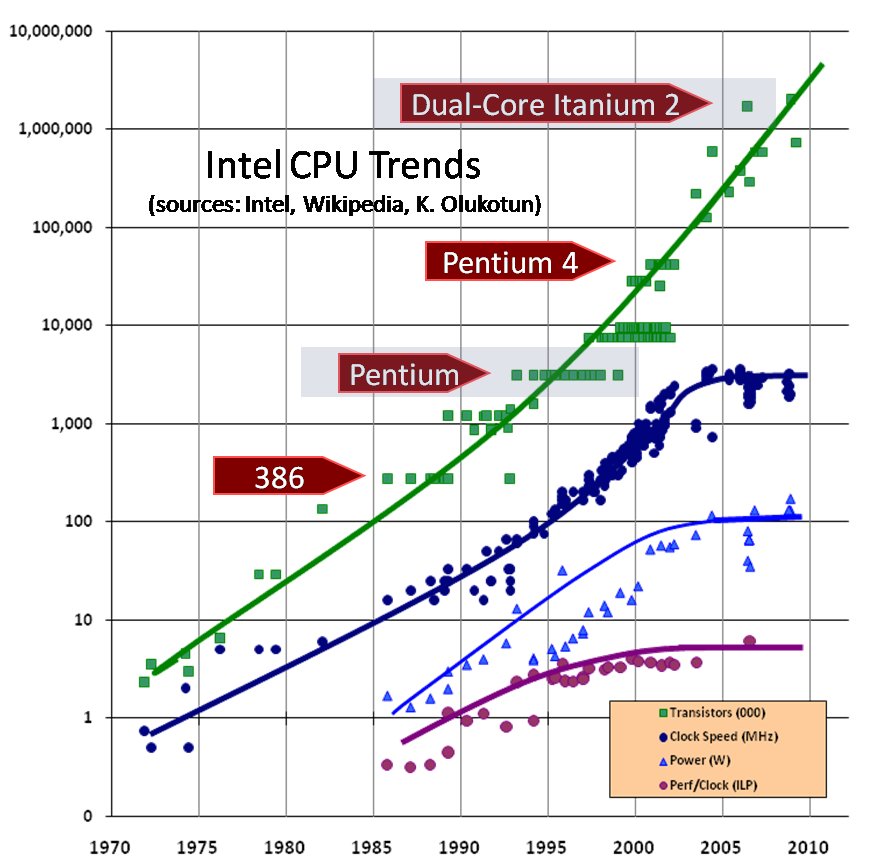
\includegraphics[width=\textwidth]{images/free-lunch-is-over.png}
    \caption{Intel CPU trends. The transistor density follows the Moore's Law, while the growth of CPU speed have stopped.~\cite{Sutter:2005:FLiO}}
    \label{fig:rne-example}
  \end{center}
\end{figure}

These chip manufacturing challenges have led into an era of \emph{dark silicon}, meaning that we cannot afford to switch all the transistors on and off at each clock cycle due to the power constraints. Before the power wall, the forefront of the silicon industry was to maximize the chip speeds. However, in the era of dark silicon, the power consumption has become perhaps the most important performance indicator, especially in the datacenter scale computing.~\cite{Sutter:2005:FLiO, Asanovic:2006:Landscape, Ributzka:2013:Concurrency, Zhang:2010:CloudComputing}

And while the silicon industry are facing various hardware development challenges, the software developers are also forced to adopt new programming paradigms to keep up with the ever increasing performance requirements.~\cite{Sutter:2005:FLiO}

\subsection{Parallel Computing}
\label{subsection:parallel-computing}

The parallelization of computing has been researched for several decades. Before the sequential execution speedup gains hit the wall, it remained a minor but important field of research, mainly in high-performance computing. Parallel-, concurrent-, and distributed computing quickly became the dominant answers for mainstream computing, to continue enjoying the benefits of the exponential computing speedups.

The \emph{parallel computing type} refers to computing in which a subparts of a program are solved at the same time. \emph{Concurrent computing}, on the other hand, executes multiple computations on overlapping time periods. In \emph{distributed computing}, the overlapping or simultaneous executions are carried out on multiple computers connected to each other.

There exist many different forms of parallel computing, often divided into four high level categories: bit-level, instruction-level, task, and data parallelism. Parallelism can be implemented in both software and hardware levels.~\cite{Culler:1997:PCA}

Bit-level parallelism refers to increasing the processor word size, thus reducing the needed number of instructions to be executed. In instruction level parallelism, the processor executes multiple instructions at the same time. Instruction level parallelism can happen in both hardware or software level.~\cite{Culler:1997:PCA}

The data parallelism refers to the simultaneous execution of the same function, on multiple cores, across the elements of the input data. Modern graphics processing units (GPU's), often implemented as wide single instruction, multiple data (SIMD) principle, are examples of data parallelism.~\cite{Culler:1997:PCA}

In contrast to data parallelism, task parallelism refers to execution of multiple cores of (possibly) completely different functions, across the same or different input data. In a typical multi-core processor, task parallelism is achieved by executing different threads or processes, on each core.~\cite{Culler:1997:PCA}

Another form of parallelism, specific to the context of network processing, is called ~\emph{Packet-level parallelism}. Network packets are typically processed on packet-by-packet basis. Most network packets are independent of each other, except for the ordering constraint for packets belonging to the same flow, thus enabling different forms of parallelism to be implemented in network processing units.~\cite{Liljeqvist:2003:Visions}

Introducing parallelism into the computing brings various new challenges in the software development. For example, the lack of a global clock, and possible failure of components demands extensive care from the developers, on top of the already challenging software development. Different frameworks and methods have been implemented, to ease the software development of efficient parallel applications. The focus of this thesis is on task level parallelism, especially in the context of packet processing applications. We will present some of the task processing frameworks more comprehensively in subsection~\ref{sec:packet-processing}.~\cite{Asanovic:2006:Landscape}

While implementing parallel systems is challenging for software developers, there are also clear limitations in the speedup gains that these methods can achieve. Amdahl's Law states the rather obvious maxima in the speedup that the program can achieve by scaling the computation over N processors. Suppose that the parallelizable proportion of a program is P (and thus the non-parallelizable proportion being P-1), then the maximum speedup, as denoted by Amdahl's Law, is:~\cite{Amdahl:1967:VSP}

\begin{equation*}
  \frac{1}{(1-P) + \frac{P}{N}}
\end{equation*}

The implication of Amdahl's Law is that the speedup of a computer program is always limited by the program's non-parallelizable proportion, thus bringing new challenges to the utilization of the available computing resources.


\section{Big Data}
\label{section:big-data}
The Internet traffic volumes are growing rapidly. For the first time, in 2010, the number of devices connected to the Internet (12.5 billion) passed the world's human population (6.8 billion). This growth is explained by the number of mobile devices (mobile phones and tablets, especially in developing countries), and the proliferation Internet of Things (IoT) devices and sensors. Cisco projects the number of mobile devices connected to the Internet, to grow up to 50 billion through 2020. IoT devices and sensors included, this number will double to over 100 billion.~\cite{Evans:2011:IoT}

According to EMC corporation sponsored IDC study~\cite{Turner:2014:Digital}, the size of the digital universe is estimated to grow ten-fold, from 4.4 zettabytes to 44 zettabytes, between 2013 and 2020. The data comes from several different sources and in many different forms. At the same time the processing requirements are growing. Everyday end users are expecting services to be delivered in higher quality near real-time, and growing number of industry, medical, and other performance critical applications are depended on the processed data.

With the enormous data masses, data diversity, and with complex processing requirements, often referred as Big Data, the traditional data processing methods become inadequate and the new performance analysis solutions become more important.


\section{Packet Processing}
\label{sec:packet-processing}

\subsection{Network Components}
Packet switching refers to a method of transmitting data in separate, suitable sized blocks, called packets, between the links of a telecommunications networks. The importance of packet switched networks is increasing in every part of the communication networks, which is explained partly by the Internet itself being an enormous packet switched network.

The Open Systems Interconnection (OSI) model is a standard conceptual model, which characterizes the communication functions involved in a general network communications of computer system. The model defines seven hierarchical layers of functional elements, between the physical interconnections (layer 1) and the software applications (layer 7).~\cite{ISO:1994:OSI}

The Internet Protocol Suite, or Transmission Control Protocol / Internet Protocol (TCP/IP), is a set of core protocols for the Internet and similar packet switched networks. It provides end-to-end data communication and specifies data packetizing, addressing, transmission, routing and receiving in the packet network. In addition to TCP and IP protocols, it provides several other network and transmission layer functionalities. The functionalities are divided into four abstraction layers: application layer, transport layer, internet layer, and link layer.~\cite{Braden:1989:TCPIP}

Internet Protocol (IP) is an essential Internet layer protocol of the Internet Protocol Suite. It provides the necessary addresses and (unreliable) delivery mechanisms for datagrams between the transmission endpoints. It is a connectionless, best-effort protocol with no error control, sequencing, or end-to-end reliability, but rather contains only the functions for packet fragmentation and delivery through the network. The packets in the IP protocol can be forwarded independent of other packets, forwarding them on-the-fly by routers.~\cite{Deering:1998:Internet}

A packet refers to the unit of data transmitted across the network. Packets consist of two parts: the header information and the payload data. Network routers use the header information to direct the packet to destination system, whereas the payload is extracted and used by the application software. All the higher layer protocols in the TCP/IP stack are encapsulated in the IP-packet's payload section.~\cite{Deering:1998:Internet}

In a conventional IP-based network architecture, the packet processing equipment and functionality is partitioned into three components: management plane, control plane, and data plane.~\cite{Chao:2007:HPS}

The control plane refers to the parts of the routing architecture, which carries and consumes the control packets needed to describe the network topology and correctly route the actual data packets. The control packets originate from and are destined for a router.~\cite{Chao:2007:HPS, Yang:2004:FCE}

The data plane, often referred as forwarding plane, deals with the actual data forwarding in the network. It defines the part of the routing architecture, which decides destination and takes action for the data arriving to it. The decision is typically determined by a look-up table, which the incoming packet is compared to. The management plane carries the traffic used for the administrative tasks of the network.~\cite{Chao:2007:HPS, Yang:2004:FCE}

\subsection{Traffic Characteristics}
The nature of the high-speed packet processing entails new types of constraints to the computing; Advanced stream processing systems are needed to process the data on-the-fly in the vicinity of the sources.~\cite{Bonomi:2012:Fog}

In the traditional von Neumann model of computing~\cite{Neumann:1993:EDVAC}, the computation is carried out by modifying the data stored in memory. However, the growing volumes of data and strict latency requirements, require not only distributing the computation, but also changes the nature of it more towards stream processing. The manipulation of the data streams passing through the system must often be done on the on-the-fly.~\cite{Bonomi:2012:Fog, Thies:2002:StreamIt}

In packet switched networks, the data streams are called \emph{flows}. Flows represent the data in specific time periods between specific network end-points. A single flow contains a large number of packets. The Internet Protocol allows each individual packet of a stream to be processed in any order, leaving the ordering of the packets to the end devices. This characteristic makes packet processing applications look like ideal for a parallel computing. However, protocols such as TCP/IP (accounting over 80\% of the Internet traffic~\cite{Fraleigh:2001:Packet}), have significant performance reductions due to reordering of packets in a single stream. For this reason, the packet processing systems often have built-in schemes, such as specialized queue management and buffering, to efficiently keep flow specific packets traversing through the queues in order.~\cite{Govind:2008:PacketReorder, Kumar:1998:RouterArchitecture}

\subsection{Networking Equipment}
Packet processing refers to the methods and concepts applied to transport data packets through the various network elements in a communication network. The network routers, switches, and other devices, such as computers and smartphones, all have their own packet processing subsystems to manage the packet traversal between the network elements. This thesis focuses on the packet routing equipment in the middle of Internet backbone.

% high performance and programmability are competing goals
% -> even mutually exclusive?

% One of the cornerstones of the Internet is the ability to connect devices together into networks, and further set of networks into internetworks. Packet switches and routers ...

% Routers and switches are the cornerstones of the Internet. They are used to connect multiple heterogeneous devices together, forming a network of devices, whereas the routers connect. heterogeneous networks into internetworks.

Traditionally, the focus in the development of network equipment -- switches, routers, and various other middleboxes -- has been to achieve high performance with very limited packet processing functionalities. The network appliances and middleboxes have typically been deployed on special purpose Application-Specific Integrated Circuits (ASIC) hardware, mainly due to high performance requirements compared to the hardware development and the absence of extensibility and flexibility requirements.~\cite{Dobrescu:2009:REP}

However, the required network functionality is becoming increasingly sophisticated. In addition to the traditional layer 2 and layer 3 routing and switching tasks, the network elements are required to handle more demanding tasks (e.g. application acceleration, encryption, and intrusion detection) all the way to layer 7. These extensions often require modified per-packet processing on the router data plane, and as the specialized network processors are difficult to extend and program, both industry and research are seeking new, more flexible networking solutions.~\cite{Egi:2009:PP, Dobrescu:2009:REP}

On the other extreme of the design spectrum, are the software routers built from general-purpose operating systems and x86 hardware platforms. The main promise of the software routers is their extensibility in the software and hardware development: the system's network functionalities, both in the data and control plane, can be modified fully by the software, thus mitigating the hardware design and development burden of the network developers.~\cite{Dobrescu:2009:REP}

The software routers also enable several other properties of the general purpose computer ecosystem. Huge manufacturing volumes and widespread supply and support chain allow much cheaper hardware prices. The rapid advances in commodity semiconductor technology, such as the state-of-the-art power management features, can provide significant advantages over the slow hardware upgrade cycles of the traditional ASIC based systems.~\cite{Dobrescu:2009:REP}

The challenge with the full software routers is the scaling the approach to high-speed networks. Between these two extremes exist design solutions, which offer much of the programmability of commodity hardware and the performance of specialized ASIC systems. Our focus in this thesis, is on the MPSoC systems consisting of these middle ground network processing units.~\cite{Dobrescu:2009:REP}

\section{Virtualization}
\label{section:virtualization}
Virtualization is an act of dividing a common set of computing resources into a multiple isolated execution environments. It enables multiple operating systems to be run, in parallel, on a single processing unit, thus alleviating the efficiency problems of parallel computing.

Before the existence of multi-user operating systems and the rapid drop in hardware cost around 1980s, the virtualization was used to allow multiple users to share the same mainframe hardware. Until the end of 1990s, it remained mainly a practice of computing industry and academic research, often requiring special hardware with explicit support for virtualization. VMWare's introduction of virtualization to the x86 architecture~\cite{Walters:1999:VVP} and the personal computer industry introduced the benefits of virtualization to the wider masses.~\cite{Bugnion:2012:BVX, Barham:2003:XAV}

\subsection{Platform Virtualization}
In the traditional, non-virtualized system, the hardware platform resources are controlled by a single operating system. Virtualization introduces a new layer, the \emph{hypervisor} (also referred as virtual machine monitor), to the software stack. The hypervisor lies underneath the existing software components, abstracting the hardware inputs, outputs, and the behavior for the use of multiple operating systems. The virtualized system is called a \emph{virtual machine}.~\cite{Uhlig:2005:IVT, Bugnion:2012:BVX, Barham:2003:XAV}

The benefits of the virtualization are numerous, mainly due to the software implementation of the virtual machines. It enables scalability and flexible migration of computation loads across different infrastructures, leading to improved hardware utilization, dynamic resource allocation and management, isolation, security, and automation.~\cite{Pearce:2013:VIS}

The virtual machines can be \emph{live migrated} over to another physical machine. While the non-virtualized systems are often under utilized, the flexibility of software enables the machines often to be run on optimal usage level. Maintenance costs can be reduced by software automation and security can be increased by additional software services, such as workload isolation. These benefits have encouraged companies to seek savings, by adopting virtualization in various contexts, ranging from the desktops and datacenters to network switching.~\cite{Uhlig:2005:IVT, Pearce:2013:VIS}

To enable fully functional virtualized environments, the virtualization of different system components, such as CPU, memory, I/O, and storage, need to be considered. CPU virtualization techniques are often divided into three categories: binary translation (full virtualization), paravirtualization, and hardware-assisted virtualization.~\cite{Bugnion:2012:BVX, Pearce:2013:VIS, Horne:2007:Understanding}

Full virtualization refers to a method where the communication between the virtualized operating system (guest) and the underlying host operating system is (nearly) completely emulated, meaning that the virtual hardware is functionally identical to the underlying machine. Unmodified guest operating systems can be run similarly as on native hardware, as the virtualization layer completely decouples them from the underlying hardware. On the other hand, the complete emulation of the hardware instructions induces performance overhead to the full virtualization.~\cite{Bugnion:2012:BVX, Barham:2003:XAV, Horne:2007:Understanding}

In paravirtualization, instead of emulating the hardware environment, the guest operating systems are executed in isolated environments. It enables the communication between the guest operating system and the hypervisor, and thus improving the performance and efficiency of the virtualization.~\cite{Barham:2003:XAV, Horne:2007:Understanding}

However, paravirtualization requires modifying the guest operating system kernel to enable direct communication with the virtualization layer monitor. For this reason, paravirtualization compatibility and portability is limited, and it can cause significant support and maintainability costs.~\cite{Barham:2003:XAV, Horne:2007:Understanding}

Hardware assisted virtualization introduces new hardware features to ease the virtualization. A common method is to provide a new privilege level below the ring 0, to allow the guest operating system to intercept and emulate privileged operations of the underlying hardware. Hardware assisted virtualization removes the need for binary translation and paravirtualization, thus, at least theoretically, solving many of the current virtualization problems.~\cite{Horne:2007:Understanding, Pearce:2013:VIS}

\subsection{Operating System Level Virtualization}
Running multiple operating systems on single hardware, as done with hypervisor-based virtualization, comes with the cost of efficiency. In many scenarios, such as high performance computing, game hosting, or MapReduce~\cite{Dean:2008:MR}, the overhead from running multiple kernels on the same machine becomes a problem. Another common method for server virtualization is to run the virtualization layer within the operating system.~\cite{Soltesz:2007:COS, Xavier:2014:Containers}

Operating system level virtualization is based on the kernel's ability to support multiple isolated user-space instances, or software \emph{containers}. Instead of emulation, programs running in containers consume the host operating system's standard system call interface, resulting in negligible virtualization overhead compared to hypervisor-based virtualization. The drawback of container based virtualization is its inflexibility; each guest must be running on the same operating system kernel as the host machine.~\cite{Soltesz:2007:COS, Xavier:2014:Containers}

Examples of operating system level virtualization implementations include for example Linux Containers (LXC)~\cite{LinuxContainers:2013:LXC}, Linux-VServer~\cite{Des:2005:Virtualization}, OpenVZ~\cite{OpenVZ:2013}, and Docker~\cite{Merkel:2014:Docker}. While most of the container implementations seem to achieve near-native performance, the management capabilities, such as, performance isolation, vary between them.

\section{Cloud Computing}
Cloud computing paradigm provides a shared pool of easily configurable and flexible computing resources via convenient, on-demand network access. One of the driving forces for cloud computing has been its promise of economics of scale. Virtualization techniques enable cloud computing centers, compared to traditional on-premise solutions, to be built using cheaper hardware, cooling, electricity, network capacity and smaller number of administrators per computer. At the same time, it alleviates the problem of inefficient resource usage, caused by the challenges discussed in section~\ref{subsection:the-end-of-free-lunch}.~\cite{Mell:2011:ccdef}

According to the definition of The National Institute of Standards and Technology, cloud computing is composed of five essential characteristics (on-demand self-service, broad network access, resource pooling, rapid elasticity, and measured service), three service models (software as a service, platform as a service, and infrastructure as a service), and four deployment models (private cloud, public cloud, community cloud, and hybrid cloud).~\cite{Mell:2011:ccdef}

%\subsection{Characteristics}
The \emph{on-demand self-service} characteristic means that the consumer of the service can provision computing resources, such as server time and network storage, automatically without requiring human interaction with each service provider. \emph{Broad network access} requires the service to be available over the network and accessible using standard mechanisms which promote use by heterogeneous platforms such as mobile phones, tablets, laptops, or personal computers. \emph{Resource pooling} refers to virtualization techniques discussed in the Section~\ref{section:virtualization}. \emph{Rapid elasticity} means that the consumer is able to elastically and automatically, provision and release the seemingly unlimited resources on demand. The last characteristic, \emph{measured service}, refers to the automatic control and optimization of the resources by metering the usage of the services.~\cite{Mell:2011:ccdef}

The characteristics of cloud computing make it tempting for both customers and service providers. From the customer perspective, it provides advantages of high computing power, cheap service costs, high performance, flexible scalability and accessibility as well as high availability. It reduces the upfront infrastructure costs for companies, allowing them to focus on their core businesses instead of on infrastructure, and getting their applications running faster, with improved manageability and less maintenance. On the other hand, it provides completely new business models for the service providers.~\cite{Mell:2011:ccdef, Dikaiakos:2009:Cloud}

%\subsection{Service Models}
The three service models divide the cloud services into logical levels based on the computing layers provided by the cloud service. Figure~\ref{fig:cloud-computing-service-models} presents the comparison these levels together with the on-premise solution. On-premise solution refers to model where the customer manages the complete computation stack.

\begin{figure}[]
  \begin{center}
    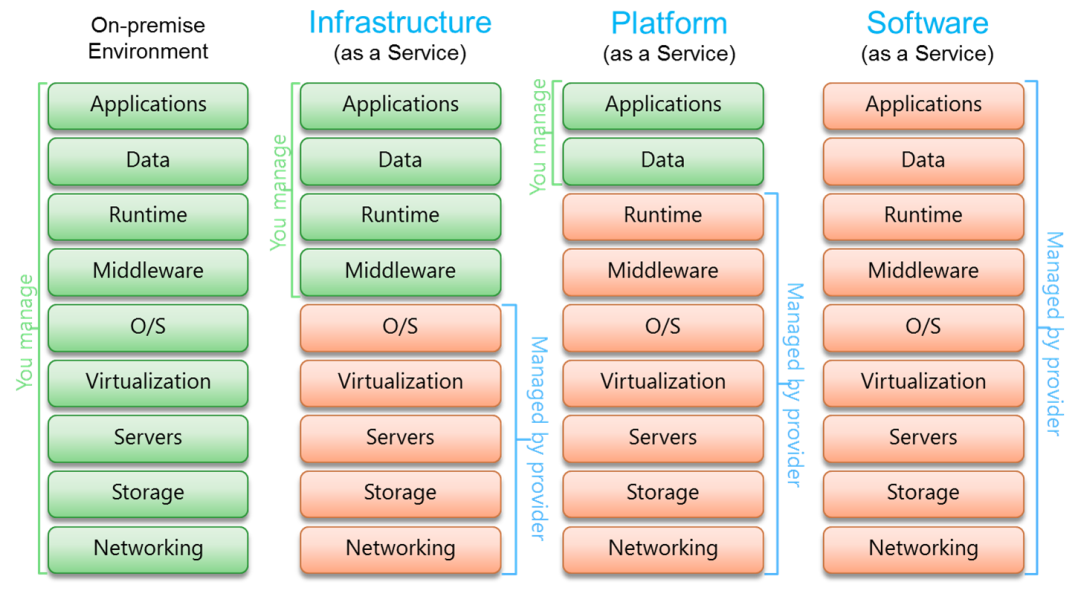
\includegraphics[width=\textwidth]{images/cloud-computing-service-models.png}
    \caption{A comparison of the three cloud service models and on-premise solution. Figure from~\cite{Lau:2011:ServiceModels}}
    \label{fig:cloud-computing-service-models}
  \end{center}
\end{figure}

The lowest of the three levels, \emph{Infrastructure as a service (IaaS)} model, provides the customer the services which abstract the details of typical hardware resources and operating systems. The computing resources are typically abstracted using a hypervisor, such as VirtualBox, KVM, Hyper-V that runs the virtual machines visible to customers as guests. Examples of IaaS providers are Amazon Web Services~\cite{Murty:2008:AWS} and Rackspace~\cite{Rackspace:2010:Inc}.~\cite{Mell:2011:ccdef}

In the next service level, \emph{Platform as a service (PaaS)} model, the service provider takes care of the platform-level middleware and runtime components. These components typically include programming-language execution environment, databases, and web servers. Google AppEngine~\cite{Sanderson:2009:GoogleAppEngine} and Windows Azure Platform~\cite{Redkar:2011:Azure} are examples of PaaS providers.~\cite{Mell:2011:ccdef}

\emph{Software as a service (SaaS)} model provides, on top of the IaaS and PaaS, the management of the application and data level. The customers access the software from cloud clients, typically web browsers via personal computers, laptops, tablets or smartphones. SaaS has become a common model for delivering wide range of different applications, such as Facebook~\cite{facebook}, Salesforce~\cite{salesforce}, and Google Gmail~\cite{Teeter:2011:Gmail}.~\cite{Mell:2011:ccdef}

%\subsection{Deployment Models}
\emph{Private Cloud} infrastructure is hosted internally by a company or organization, targeting a specific set of customers. Private clouds are typically more affordable to setup and offer more flexibility, while also providing the companies full privacy on their data and applications. \emph{Public Cloud}, on the other hand, is exposed to any customer over a public network. The data, applications and other resources are stored over the service provider's data center, and thus the security has to be considered. The underlying infrastructure is often similar between these two models.~\cite{Mell:2011:ccdef}

The cloud service can also be a combination of the public and private clouds. This kind of deployment model is referred to as a \emph{hybrid cloud}. Hybrid cloud allows the utilization of the flexibility and cost of the public cloud solutions, while at the same time maintaining the security sensitive data in their own infrastructure. \emph{Community cloud} refers to cloud infrastructure that is shared between multiple organizations, typically with common security, jurisdiction, and compliance concerns in mind. Community clouds can be hosted and managed either internally or externally from the sharing organizations.~\cite{Mell:2011:ccdef}

\subsection{Energy Consumption}
The power consumption has become the major concerns in the design of today's warehouse scale datacenters. In 2005, the world's server power demand (including cooling and auxiliary infrastructure) was about 14,000MW, resulting in about \$7.2B eletcricity costs. Majority of these costs come from cooling, which is the consequence of the heat generated by the computing resources such as CPU, memory, storage, and networking.~\cite{Koomey:2007:PC, Fan:2007:PPW}

Virtualized datacenters can greatly increase the usage rates of computing resources, decreasing the total server energy consumption. However, the benefits of cloud computing are tightly coupled to the scale of the individual datacenters. While the total energy consumption is reduced, the energy usage of individual datacenters are often huge.~\cite{Hoelzle:2009:DCI}

The datacenter costs can be optimized by more efficient hardware implementations and increased usage rates, but companies also have to consider different non-technical solutions. The design and construction of warehouse scale datacenters should be treated similarly to traditional factories. Size, location, and physical design of the datacenter can have considerable effect on the costs.~\cite{Hoelzle:2009:DCI}

Google's Summa datacenter is a good example of the scale of the cloud datacenter. Google, a company residing in California, invested over \$200M to build a datacenter in Hamina, Finland. The benefits from Finland's energy infrastructure, cold climate, developable land and available workforce, outweighed all the negative qualities of building the datacenter on the other continent, nearly 9000km away from the company's head quarters.~\cite{Google:2016:Summa}

\subsection{Datacenter Networks}
For compatibility and cost reasons, datacenter networks are often built from commodity Ethernet switches and routers (scaling out), rather than from expensive high-end hardware (scaling in). Due to the limits in the switch port densities even in the high-end hardware, the traditional single rooted topologies are replaced with multi-rooted tree topologies such as fat-tree or leaf-spine. Multi-rooted network design allows to scale the data center networks' bisection bandwidth by adding new spine switches into the network.~\cite{Al-Fares:2010:SO, Al-Fares:2008:SCD}

Cloud computing datacenters can consist of hundreds of thousands of servers, supporting large variety of services, such as high performance computing, MapReduce~\cite{Dean:2008:MR} and web services. Many of these applications have several inter-dependent components divided across the servers. Thus, the inter-node network bandwidth has become the major bottleneck in data centers.~\cite{Al-Fares:2008:SCD}

To efficiently utilize datacenter resources, and to answer the required performance guarantees, efficient network traffic load balancing mechanisms are needed. Several different proposals, such as CONGA~\cite{Alizadeh:2014:Conga},  Presto~\cite{He:2015:Presto}, and Hedera~\cite{Al-Fares:2010:Hedera}, have been made to overcome the issues of traditional hash based schemes.

\section{Fog Computing}
\label{section:fog-computing}

% The IT and Telecommunication Networking evolutions are coming closer to each other.
% -> new possibilities
% -> computation is moving to the network edge, closer to the end user and sensors.

% ``Mobile-edge Computing can be seen as a cloud server running at the edge of a mobile network and performing specific tasks that could not be achieved with traditional network infrastructure. Machine-to-Machine gateway and control functions are one example, but there are many others.''

% ``Move the computation code to the data, not the other way''

While the benefits of Cloud Computing provide efficient alternative to the traditional on-premise solutions, there are certain issues, which have to be addressed to enable a new breed of ever demanding applications and services. Characteristics, such as mobility, geo-distribution, location awareness and low latency are intractable to achieve due to the centralized nature of cloud computing. The proliferation of devices and sensors have led to a situation where the data are produced faster than can be transmitted or stored.~\cite{Bonomi:2012:Fog, Vaquero:2014:FYW}

Fog computing is an extension to the traditional cloud computing architecture, where parts of the cloud computing services, mainly computation, storage, and networking, are carried out in the edge of the communication network. It is defined to provide the following characteristics on top of the existing cloud computing architectures: low latency and location awareness; wide-spread geographical distribution; mobility; very large number of nodes, predominant role of wireless access, strong presence of streaming and real time applications, heterogeneity.~\cite{Bonomi:2012:Fog}

High virtualization and efficient stream processing are the key elements for successful fog computing.

Until recently, the typical network architectures have been implemented on proprietary or special purpose hardware. The growing networking traffic and competition in communication services have led to the development of software based solutions. Software based solutions enable flexible and extensible networking, and measure up the tight standards for stability, protocol adherence, and quality, previously achieved only with the hardware solutions.~\cite{Kim:2013:SDN}

The main enabling technologies of fog computing are the software-defined networking (SDN), and further the network functions virtualization (NFV). Software defined networking separates the data plane and the control plane functionalities of the network, making the data plane switches simple packet forwarding devices, while leaving the routing decision control logic for the control plane. Thus the network control becomes directly programmable, centrally managed, programmatically configurable, and vendor agnostic, amongst many other benefits from softwareization.~\cite{Kim:2013:SDN}

SDN is often complemented with network functions virtualization. In NFV, the network devices are virtualized (using similar techniques as discussed in section~\ref{section:virtualization}) and the network functionalities of the devices are implemented in software packages.~\cite{Demestichas:2013:NFV}

Long Term Evolution (LTE)~\cite{Sesia:2009:LTE} and Evolved Packet Core (EPC) work as a natural platforms for the fog's edge data centers. Small cloud stations can be deployed to the EPCs, and the routers can be utilized as the virtualization infrastructure. This also enables the application services to be co-located where needed.~\cite{Vaquero:2014:FYW}

%%% Local Variables:
%%% mode: latex
%%% TeX-master: "thesis-hartikainen"
%%% End:

\chapter{System Performance Analysis and Simulation}
\label{chapter:system-performance-analysis-and-simulation}

In this thesis, we study and evaluate the performance of a distributed stream computing system. Our evaluations are based on the modeling and simulation techniques, while measurements are also needed to build the model. Similarly to many other packet processing system studies~\cite{cavium:2010:fundamentals}, we are mostly interested in the communication delays, namely throughput and latency, of the system.

This chapter introduces the methods used in our experiments. We will start by introducing the common performance analysis techniques and metrics, and then further examine the modeling and simulation techniques. After that, \todo[inline]{yadayada}

\section{Performance Analysis}
For almost every computer system -- whether it be a high performance application on the cloud~\cite{jackson:2010:HPCOC} or an army fuel-supply system~\cite{sabuncuoglu:2005:TAS} -- the performance is one of the most sought-after criterion. To achieve the highest performance for the lowest cost, different performance evaluation techniques are required at different system life cycle stages. The choice of evaluation criteria and techniques, used to evaluate the system performance, vary between systems. These two choices are discussed in the following subsections.~\cite{jain:1991:AOCSPA}

\subsection{Evaluation Techniques}
Performance evaluation can be done using various techniques. These techniques are generally divided into three categories: analytical modeling, simulation, and measurement. The former two techniques are based on symbolic models of the real-life system, whereas the measurements are done on the system itself. Analytical approaches use mathematical methods to solve the model, and simulation imitates the operation of the system by executing the model on a simulator~\cite{Banks:2010:DES}. Measurements are done by instrumenting the real system with various hardware and software tools.~\cite{jain:1991:AOCSPA}

No strict programmatic rules can be given to select the right technique. However, there are some considerations that can be used to guide the decisions: system life-cycle stage; available resources, such as time, money and tools; required level of accuracy; trade-off evaluation; and saleability.~\cite{jain:1991:AOCSPA}

The life-cycle stage of the system is often the first consideration. In early design stage, the evaluation is often done by using analytical methods or simulation, as it is impossible to measure a yet non-existing system. Measurements are, thus, often used for improving an existing systems.~\cite{jain:1991:AOCSPA}

Available resources also dictate the technique selection. Running the measurements and simulations are often more time consuming~\cite{Fujimoto:1990:PDE} than the analytic approach, and the required time can be hard to predict. They both also require special equipment and tools, which are expensive and need special skills to operate. The analytical methods are generally considered less time consuming and less expensive than measurement and simulation.~\cite{jain:1991:AOCSPA}

\todo[inline]{PDES stuff: parallelizing is hard - scaling simulation is non-trivial?}

The required level of accuracy should also be considered. For analytical models to be solvable, they often have to be very simple abstractions of the original system. Thus, the results of the analytical methods are often approximate. Simulations, like analytical methods, are abstract, but often much closer to the real system. Even measurements can produce results that do not agree with the actual system behavior. Generally measurements can be considered the most accurate, and analytical methods more inaccurate than the simulation. The accuracy of simulations and measurements can often be enhanced by spending more time and money to them.~\cite{jain:1991:AOCSPA}

Different evaluation techniques are often used together. Taking advantage of two or more methods simultaneously can be used to validate and verify the analysis results. On the other hand, different methods can be used to complement each other to enhance the analysis process.~\cite{jain:1991:AOCSPA}

\todo[inline]{performance analysis like art?}

\subsection{Performance Metrics}
Every performance study needs a set of performance criteria or metrics, which vary with the service provided by the system. Service requests made to the system produce different outcomes: the system either performs the service -- correctly or incorrectly -- or refuses to perform it. The metrics associated with these outcomes are called speed, reliability, and availability, respectively.~\cite{jain:1991:AOCSPA}

When the service result is correct, the performance metrics are used to measure the responsiveness, productivity and utilization of the system. For example, in a network packet processing system, the responsiveness could be measured as the packet response time, the productivity as the throughput, and the utilization as the percentage of time the cores are busy~\cite{cavium:2010:fundamentals}.~\cite{jain:1991:AOCSPA}

If the service result is incorrect, the metrics describe the probabilities of the error. For example, how probably an unintentional packet drops or out-of-orderings occur. When the system fails to perform requested service, it is helpful the classify the different causes of failure, and determine the probability and the duration for each.~\cite{jain:1991:AOCSPA}

It should be noted that many systems provide multiple services, and the number of metrics can be large. Also, different evaluation techniques provide different metrics at different times of the service. For example, some simulators allow white-box-like view of the system states during the simulation, whereas, with analytical methods, the details of the system are often unavailable.~\cite{jain:1991:AOCSPA}~\cite{TODO: find reference for the white-box black-box stuff}

\section{Simulation}
This sections describes the basic principles related to simulation. Note that, despite the most of the examples in this chapter being about computing, simulation is widely used in several other contexts, even outside science. The concepts described below, e.g. entities, attributes, or activities, to name a few, have different realizations from system to system.

Simulation is an artificial imitation of the operation of a real-life system over time. The system behavior is studied by developing a simulation model, based on a set assumptions concerning the characteristics and functions of the system. The assumptions are presented in mathematical, logical, and symbolic relationships between the objects of interest of the system. An artificial operation history is generated by executing the simulation model, generally on a simulator program, with respect to system input and time. Data are collected from the simulation similarly as if the real system was being measured.

\subsection{System components and environment}
\label{sec:syst-comp-envir}

In simulation, a \emph{system} is defined to be a set of objects that work together, in regular interaction or interdependence, to accomplish some goal or purpose. Every system is a subsystem of broader \emph{system environment}, whose changes can affect the system. For every simulation study, a \emph{boundary} between the system and its environment must be set.~\cite{Banks:2010:DES}

For example, computer systems are often enormously complex. The complexity is managed by designing them as a hierarchy of smaller subsystems, and combining them with compatible interfaces. In a study of a network processing system, such as~\cite{cavium OCTEON}, the higher level system can be viewed to consist of several processors, auxiliary memory, memory controllers, and other smaller subsystems. These subsystems can further be viewed as a set of smaller subsystems of subsystems: the processor has several processing cores, each core consists of different functional units, and each functional unit consists of logical circuitry.~\cite{Banks:2010:DES}

The objects of interest in a system are called \emph{entities}, which are associated with a set \emph{attributes}. An \emph{activity} is a specified length time period. A system \emph{state} completely describes the system at any given time of a specific study. The system state might be changed by an immediate occurrences called \emph{events}. The events affecting the system are divided into two groups by their source: \emph{endogenous} events occur within the system under study, and \emph{exogenous} events occur in the system environment.~\cite{Banks:2010:DES}

Continuing with the above example, each of the mentioned components can be seen as the entities of the system. There are several activities and events at different levels of the system. At the higher level, these can be seen as the packets flowing through the system: writes and reads to the memory, execution on different processors, and queueing for the processor time. At a lower level, these could be the computation done by the logical units or the flipping of the transistors' state.

Systems can be divided into two categories as per the type of their state change: discrete systems and continuous systems. In a \emph{discrete system}, the system's state changes only at a discrete time points, and in a \emph{continuous system}, the state change is continuous over time. In practice, almost every system is a combination of both continuous and discrete changes. These systems are often classified by the dominant type.~\cite{Banks:2010:DES}

\subsection{Simulation Model}
\label{sec:simulation-model}

Simulation \emph{model} is a representation of either hypothetical or real-life system under study. By its definition~\cite{Encyclopedia of computer science}, the model should be a simplified representation of the original system. In simulation, it should represent the studied system with enough detail to provide relevant conclusions and, at the same time, only consider those details that affect the investigated problem. The decision between the level of accuracy and abstraction usually requires knowledge of the system under modeling.~\cite{Banks:2010:DES}

Like with the system representation, the basic building blocks of the simulation model are entities, attributes, activities and events. The model does not necessarily contain the exact replica of the components of the system, but rather simplified components that represent the system with enough detail.~\cite{Banks:2010:DES}

In the example study of network processing unit, the likely goals would be to determine the packet throughput and latency of the system. In that case, the system could be modeled with sufficient accuracy by omitting all the lower level details of the CPU. On the other hand, a detailed performance study of a specific CPU might require even the minute details of the functional units or logical circuitry.~\cite{TODO: find some simulation example for this}

The models may be categorized as being static or dynamic, and deterministic or stochastic. Static simulation models represent a steady-state time-invariant systems, whereas the dynamic simulation models represent systems as time-variant. Deterministic models contain no random variables, meaning that for the known set of inputs, the simulation result will be a unique set of outputs. Stochastic models on the other hand include random variables, thus leading to a random set of outputs.~\cite{Banks:2010:DES}

Simulation models are further divided into discrete and continuous, analogously with the discrete and continuous systems described in Section \ref{sec:syst-comp-envir}. However, it is possible to model continuous systems with discrete models, and vice versa. Just as the real-life systems, the simulation models can be a mix of both continuous and discrete models.~\cite{Banks:2010:DES}

Three different simulation advancement designs are presented in~\cite{peros:2009:simulation}: event-advance, unit-time advance and activity based. In event-advance design the system state changes only when the event occurs. Thus the system state advances from snapshot to snapshot, meaning that the state is unchanged between two successive events. In unit-time advance design, the master clock is advanced in fixed time increments. Activity based design is a continuous design method, which models the system as a set of conditions that determine when the activities start or stop.~\cite{peros:2009:simulation}

\subsection{Monitoring}

To make conclusion about simulation, the information about the simulation system needs to be gathered. Similarily to the measurement based techniques, the system is instrumented and the data are saved during the execution.

There are two generally used approaches for gathering simulation metrics: trace-based and on-the-fly. The tracing approaches produce raw data from the execution, which are then often post-processed in suitable way. In on-the-fly approaches, the simulator program aggregates the data during the simulation, thus reducing the amount of output.\todo{cite, jain?}

\todo[inline]{add the resource network stuff somewhere?}

\section{Simulator Software}
\todo[inline]{describe available simulator software here?}

\todo[inline]{CloudSim: Provides tools for simulation IaaS.
  Provides configuration for data centers, hosts and virtual machines.
Different policies for creating host VM's, assigning VM's to hosts, VM resource allocation etc
}

\todo[inline]{Rsim: More detailed hardware simulation, with focus on ILP effects of processors
      Detailed shared-memory multiprocessor models
      They show that the previous simple-processor-models cannot demonstrate the complicated dynamically scheduled processors with sufficient detail.}

\todo[inline]{Simics: ``Reliable performance estimates require simulation of the full system''
        Their simulator includes device models accurate enough to run unmodified operating system kernels, firmware and device driver.
        They simulate a network of heterogeneous computers.
        Commercial product
        Two dimensional classification:
          scope (what is modeled),
          abstraction level (level at which the system is modeled)
            two perspectives: functional, timing (performance)}

\todo[inline]{SimpleScalar:
  Hardware development is often accelerated by software simulations of the hardware under development.
  Basic idea: Implement a software model of the hardware, stress then with appropriate workload
  Gains: The availability of the simulation model is much faster than building the hardware. Thus the hardware can be tested faster. Shorter time to market, cut down development costs.
  Simulation modeling is driven by three factors: performance, flexibility, detail
    Performance measures the system's ability to process workload
    Flexibility reflects the ability to modify the models, enabling measurements of different designs
    Detail means the level of abstraction the model captures from the actual system
    -> Getting all three is hard, practically impossible.
    -> trade offs}

% In discrete-event simulation models the system's state at each point of discrete times. The system is modeled in terms of the entities flowing through the system utilizing other entities that represent the system resources.~\cite{Banks:2010:DES}

% DES is one way of progressing the simulation

% The idea of the general model is expanded with queues, event lists, delay, clock.


%%% Local Variables:
%%% mode: latex
%%% TeX-master: "thesis-hartikainen"
%%% End:

\chapter{Performance Simulation Environment}
\label{chapter:performance-simulation-environment}

This chapter describes Performance Simulation Environment (PSE) and its usage for performance analysis of a stream computing system. We begin with an overview of PSE tools and concepts, and continue by describing the three components of a PSE model. After that, we go through the simulation and monitoring of PSE applications. Finally, we address the problems and deficiencies, namely the lack of global queue scheduling, that needed to be resolved before PSE could be used for performance analysis of a stream computing system.

\section{Toolset Overview}
\label{sec:toolset-overview}

PSE is a toolset and simulation environment for dynamic performance analysis of, initially designed but not limited to, parallel computing systems. The tools consist of graphical model editors, compiler tools, and discrete event simulator runtime.

\begin{figure}[]
  \begin{center}
    %% \input{images/pse-toolset.tex}
    \missingfigure{\Huge pse toolset overview}
    \caption{PSE toolset includes the model editors, compiler tools and the simulator runtime libraries.}
    \label{fig:pse-toolset}
  \end{center}
\end{figure}

The graphical model editors -- workload editor, wle; task graph editor, tge; sequence chart editor, sce; and resource network editor, rne -- are used to build and edit the PSE model representation of a system. Each model editor has a corresponding compiler (wlc, tgc, scc, and rnc, respectively), that is used to compile the textual model representations into C-code.

The generated model code and the built-in simulator runtime libraries are compiled into an executable simulator program, using generic C compiler such as GCC~\cite{stallman:2009:gcc}. The resulting program can be run on top of Linux operating system on commodity hardware.

\section{PSE Model}

In PSE, the system under study is modeled as a resource network~\cite{Menasce:1994:CPP:174466}. The complete model consists of three main components: resource provision model, resource usage model and workload model. Each of the components are presented as directed graphs, where the nodes represent model entities and the arcs represent the possible flow directions of the tasks.

The resource provision model represents the available system resources, for example a computer hardware. The graph nodes represent resource entities, and arcs represent the possible usage order of the resources. The resources are consumed by the tasks, generated by the workload model and guided by the resouce usage model.

A resource can be either active or passive. Active resources provide service and introduce service delay to the tasks using them. An example of active resource could be a processor core, which can serve certain amount of processing cycles per unit time. Passive resources do not induce direct delay to the jobs, but their possession is required to access certain other resources. Locks could be an example of passive resource.

\begin{figure}[]
  \begin{center}
    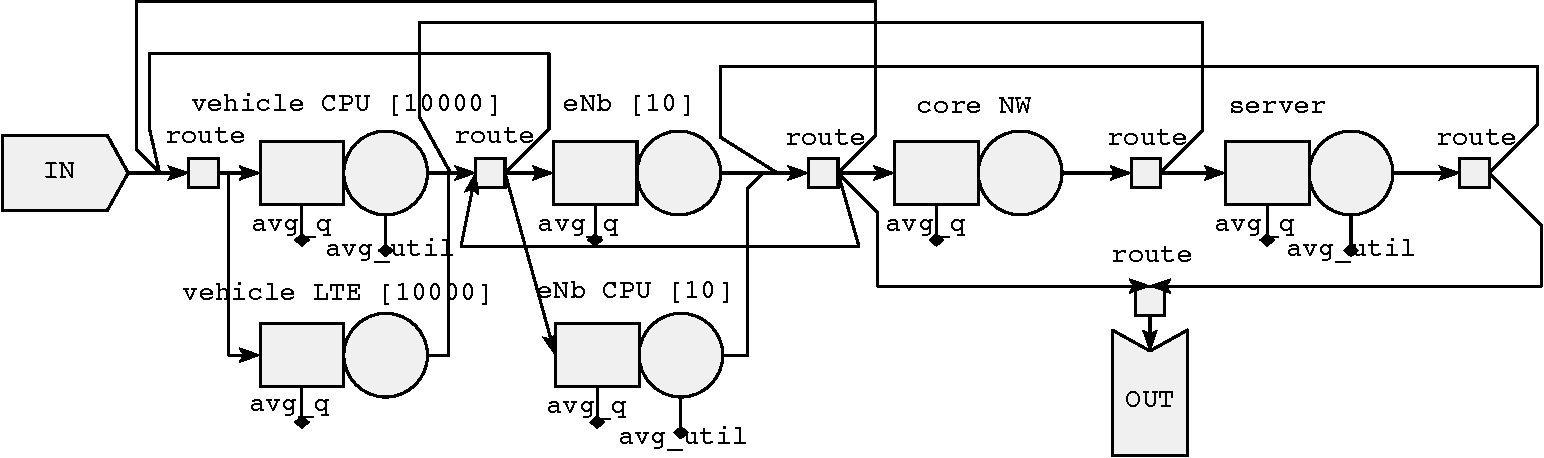
\includegraphics[width=\textwidth]{images/pse-rne-example-crop.pdf}
    \caption{An example of resource provision model.TODO: cite and add caption}
    \label{fig:resource-provision-model}
  \end{center}

\end{figure}

Figure \ref{fig:resource-provision-model} presents an example of a resource provision model ...
\todo[inline]{Explain the figure}

The resource usage models can be presented as message sequence charts or tasks graphs. We omit the discussion of the sequence chart in this thesis. Task graph is a presentation of the resource usage of the tasks arriving to the system. The nodes in the task graph can be divided into three categories: execution nodes describe the resource usage events and activities, branching nodes conditionally guide the tasks through the graph, and fork/join nodes present task subdivision. The arcs present the flow of control in the system.

\begin{figure}[]
  \begin{center}
    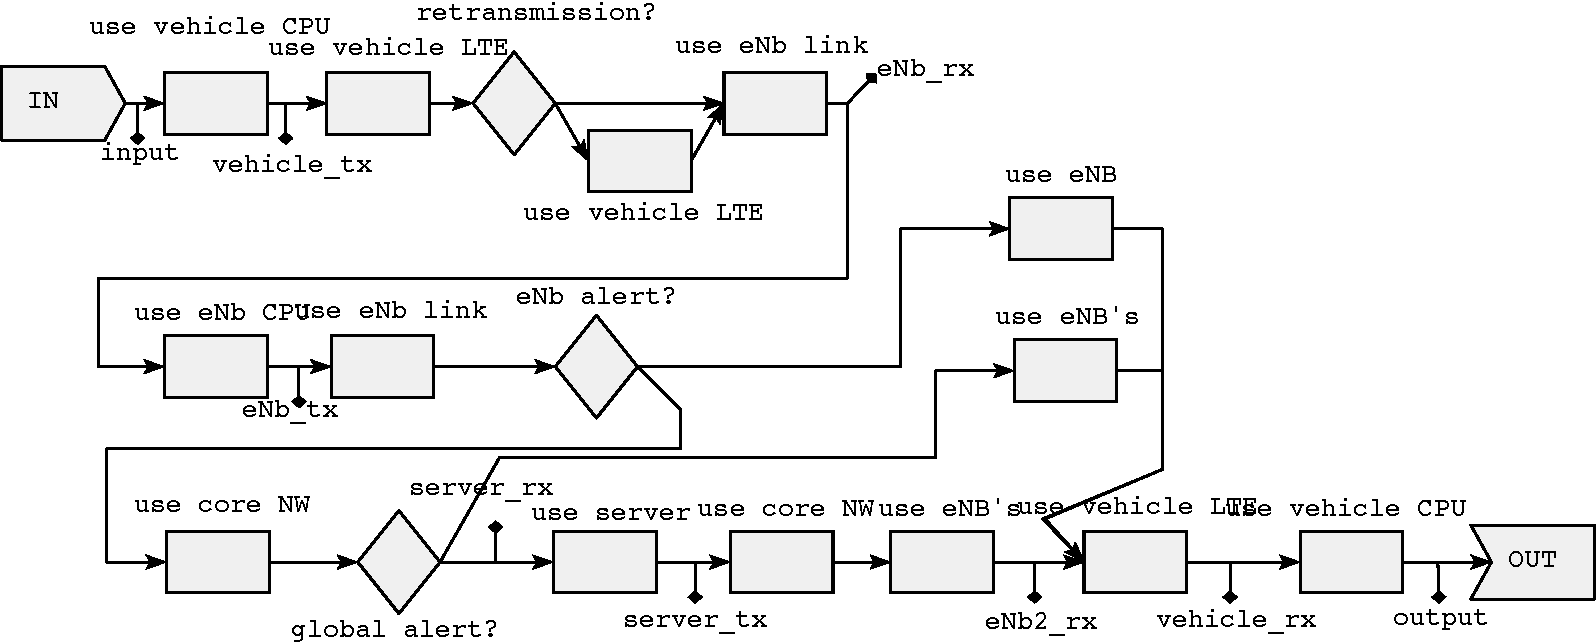
\includegraphics[width=\textwidth]{images/pse-tge-example-crop.pdf}
    \caption{An example of resource usage model.TODO: cite and add caption}
    \label{fig:resource-usage-model}
  \end{center}
\end{figure}

Figure \ref{fig:resource-usage-model} presents an example of a resource usage model ...
\todo[inline]{Explain the figure}

The workload model generates tasks, which traverse through the system according to the rules defined in the resource usage model, consuming the resources defined in the resource provision model. The nodes in the workload graph describe the task generating processes, and the arcs define the relationships between them. The graph representing the workload model must be acyclic.

The event spawn rate can be constant or random (specified for example with probability distribution).

When an event is spawned, it progresses through the resource provision model triggering the resource usages. -> gets delayed.

\begin{figure}[]
  \begin{center}
    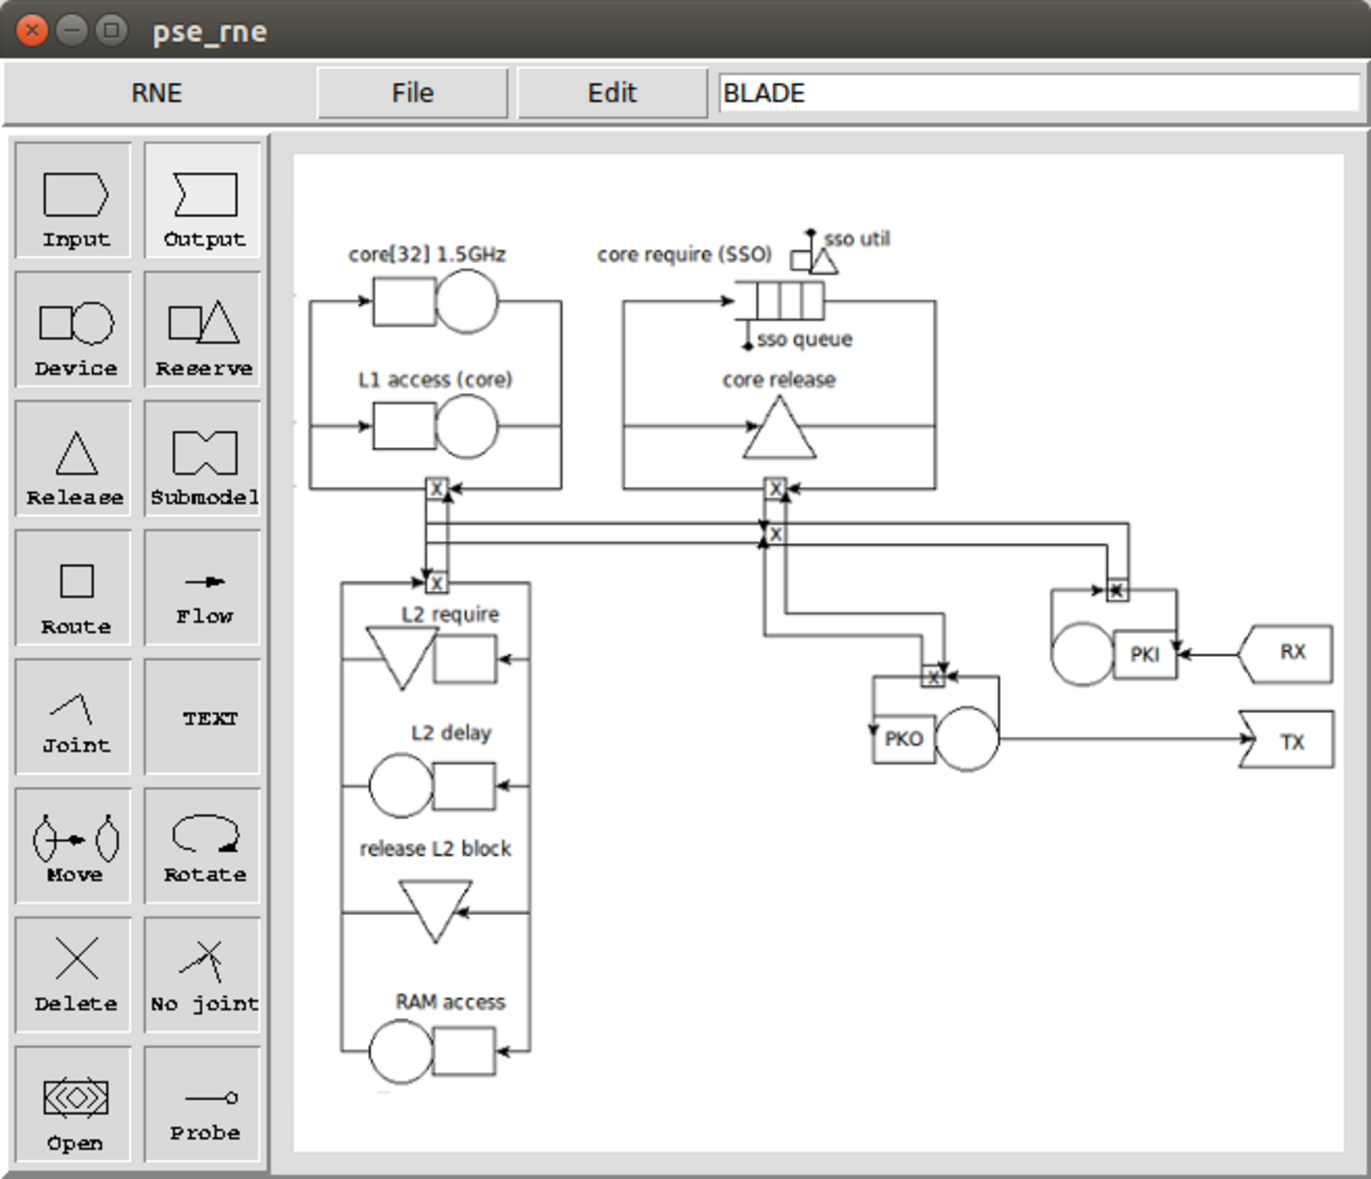
\includegraphics[width=\textwidth]{images/rne-example.pdf}
    \caption{The graphical user interface of the resource network editor. The actual resource network model is presented in the middle, and the toolbar on the left.}
    \label{fig:rne-example}
  \end{center}
\end{figure}

\section{Monitoring}

PSE has flexible, built-in, monitoring support which offers both trace-based and on-the-fly monitoring. The monitoring is controlled by attaching probes to the nodes and vertices of the simulation model nodes. It can be done on all the three model levels and practically every simulation system state change can be captured. There are essentially two different types of probes in PSE: the trace probes for trace-based measurements, and the metric probes for on-the-fly measurements.

In the resource provision model, the probes can be attached to two different parts of the resourse, to measure either the resource utilization, or its queue size. The trace probes capture every change in the resource utilization or queue size, whereas the metric trace produce aggregate only the descriptive statistics. The descriptive statistics currently include mean, standard deviation, mininimum, maximum, sum, and total number of tasks that passed through.

In the resource usage model, the probes can be attached to the model edges, producing a timestamped trace whenever a task travels the edge. The timing can be either absolute time with respect to the global system time, or relative to the process start time. The metric probes can be used to capture the average times of all tasks relative to the start of the process. Probes in the workload model are used to control the grouping of the resource usage and resource provision probes.

The probe output is written in a text file defined in the probe node attributes. The trace probes write the output in Comma-Separated Values~\cite{Shafranovic:2005:CSV} format, and the metrics traces write a standard descriptive statistics output. Using the trace based probing can substantially slow down the simulation, as the output files easily grow very large, slowing down the writes. Thus, whenever the complete trace log is not needed, it is recommended to use the metric based probing. Figure~\ref{fig:full-model} in section~\ref{sec:simulation-model} presents examples of probes attached to core-, memory- and SSO units in the hardware model as well as the in- and out- probes int the software model.

\section{Resource Network Simulator}
\label{sec:resource-network-simulator}

Performance Simulation Environment provides a discrete event simulator engine, named resource network simulator (RNS). The final simulator program is created by compiling the RNS runtime libraries together with the generated simulation model code. The simulator engine manages the simulation execution, i.e. tracks the global simulation time, schedules tasks and manages the system monitoring.

The simulator inputs are generated by the workload model, which spawns a new system thread for each generated input. The input can be either a control input or an actual workload task. The former of these are used for the simulation control, for example changing or resetting the simulation time or monitoring metrics. The latter are the actual task entities presented in section~\ref{sec:simulation-model}.

\subsection{Simulator Engine}
\label{sec:simulator-engine}

\begin{figure}[]
  \begin{center}
    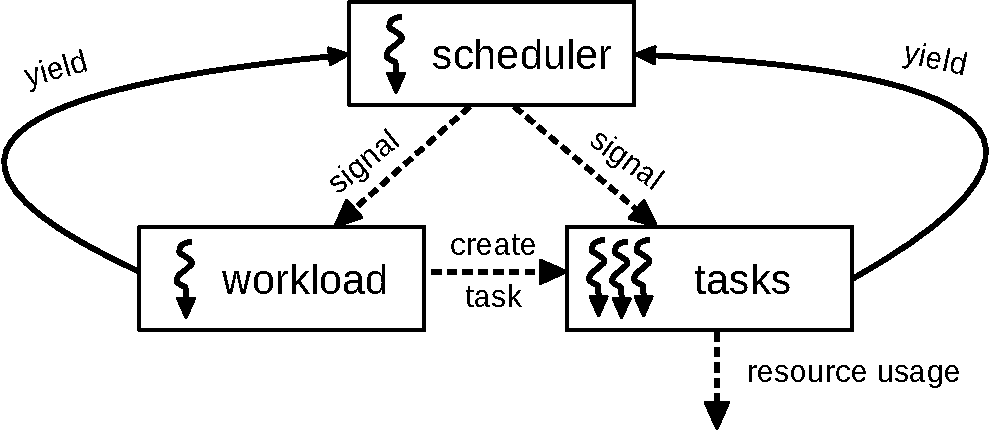
\includegraphics[width=\textwidth]{images/rns-threads-crop.pdf}
    \caption{The thread cycle of performance simulation environment's resource network simulator engine.}
    \label{fig:rns-threads}
  \end{center}
\end{figure}

Figure~\ref{fig:rns-threads} represents the model of execution in the RNS engine. The RNS scheduler, running in an infinite loop in its own thread, signals the workload threads or the task threads, based on the trigger time. RNS advances in the event-advance manner, meaning that the thread with the smallest trigger time, based on the scheduler's internal bookkeeping, gets always executed first.

The workload threads spawn new tasks to the actual taskpool, according to the code generated from the workload model. The execution of the taskpool threads advance the actual simulator, consuming the resources models based on the values defined in the resource usage model. Each time a thread's task encounters an event that is dependent on the other thread's execution, it yields the execution to the scheduler thread, which then signals the thread, again, with the smallest trigger time.

%%% Local Variables:
%%% mode: latex
%%% TeX-master: "thesis-hartikainen"
%%% End:

\chapter{Packet Processing Systems}
\label{chapter:packet-processing-systems}

This chapter presents the general methodology of packet processing and network processing units. We begin by describing the general packet processing framework used in network processors. After that, we present the packet flow handling and quality of service methods, emphasizing the importance of packet buffering and queuing theory in the packet processing. Further, we present an overview of the hardware architecture and programming models used in packet processing units.

Finally we will have a closer look on a specific network processing unit, Cavium OCTEON II CN6880, and instrument the system to obtain the required information to model the system. Two different measurements will be done: one to measure the communication latencies, and another to measure the memory latencies and throughput.

\section{General Packet Processing Framework}

A general packet processing framework consists of three primary aspects: packet processing functions, packet direction (ingress, egress, or combination of both), and packet processing paths. These three aspects are depicted in Figure~\ref{fig:general-packet-processing-framework}. The packets enter the system from the left, from the physical line interface (ingress direction), and follow either the slow or the fast path. The packets are then forwarded either to the switch fabric or back to the physical line interface (egress direction).~\cite{Giladi:2008:Network}

\begin{figure}[]
  \begin{center}
    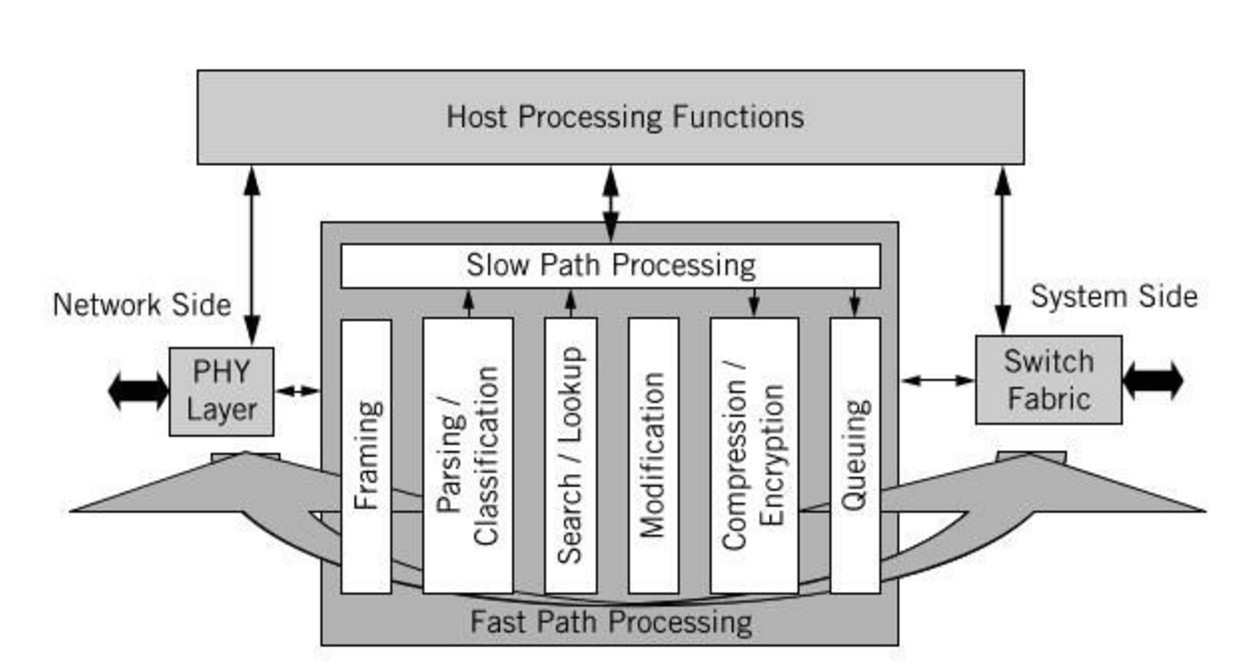
\includegraphics[width=\textwidth]{images/general-packet-processing-framework.png}
    \caption{A general packet processing framework. Figure from~\cite{Giladi:2008:Network}}
    \label{fig:general-packet-processing-framework}
  \end{center}
\end{figure}

\subsection{Ingress and Egress}
Ingress and egress refer to the packet processing done for the packets entering the network processor from the network, or packets leaving the network processor to the network, respectively. Ingress and egress processing, although not necessarily being clearly separated in modern systems, play an important role in the network processing units. The unclear separation of these phases is due to the various different implementations in today's network processing units. Some processors have one processing direction, from packet input to its output, possibly happening through the same interface. Other implementations might not have distinguishable elements that target ingress or egress processing.~\cite{Giladi:2008:Network}

Figure~\ref{fig:ingress-egress} outlines the basic two-part equipment implementation scheme, called half-duplex, for packet ingress-egress processing. The first part of the picture depicts the line cards for receiving/transmitting the packets from/to the network. The second part consists of switching fabric, service cards, and other processing functions and mechanisms that packets go through internally.

\begin{figure}[]
  \begin{center}
    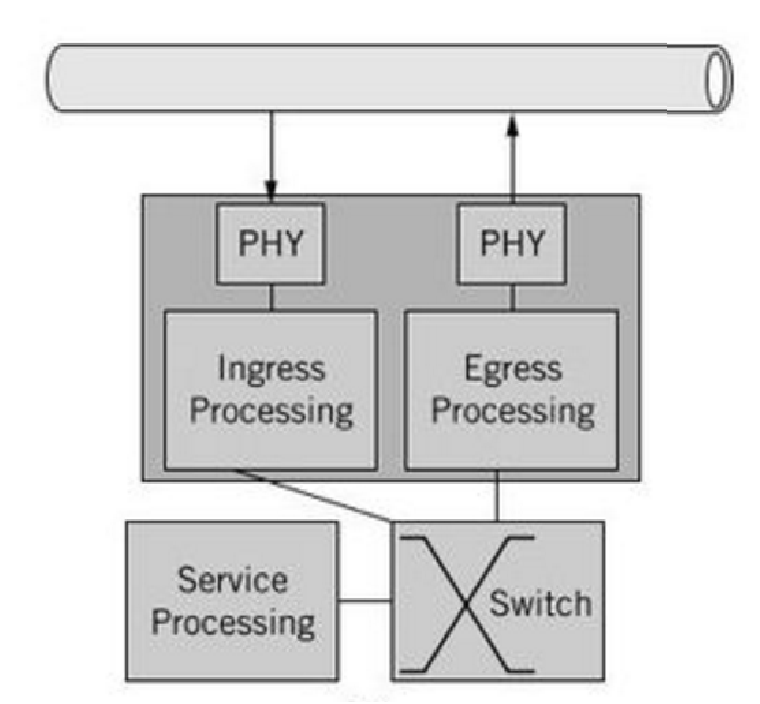
\includegraphics[width=.6\textwidth]{images/ingress-egress.pdf}
    \caption{Two part ingres-egress scheme. Figure from~\cite{Giladi:2008:Network}}
    \label{fig:ingress-egress}
  \end{center}
\end{figure}

Half-duplex processing consists of two dedicated processors for each direction. The functions executed on the ingress packets and egress packets can be distinguished, in which case the network processing unit often consists of separated processing paths for the two ways. Typical ingress processing tasks consists of, for example, error checking, classification, traffic management, header manipulations, and prioritization and queuing. Packet egress tasks, on the other hand, include checksum calculation, address lookup, packet forwarding, segmentation and fragmentation, traffic management, and packet prioritozation and queuing.~\cite{Giladi:2008:Network}

\subsection{Processing Paths}
In many cases, the packets flowing through the network processing unit need to be processed at wire speed, meaning that the number of packet leaving and arriving the processing unit must be equal at certain time interval. The introduction of increasing Ethernet speeds imposes strict constraints for the network processors. While the control- and management plane traffic can often be processed with fairly non-trivial solutions, the main bottleneck, to keep up with the scalability of optical transmission technology, is the data plane processing.~\cite{Giladi:2008:Network}

The comparison of the speeds of Ethernet based transport networks and the processor speeds gives a perspective of the packet processing requirements. A typical Ethernet link in the network backbone, with 100Gbps speed and minimum frame size of 64 bytes, leaves the packet processing system 6.7ns to process each packet.~\cite{Giladi:2008:Network}

Even in the most trivial packet processing applications, this processing requires several different processing steps. For each packet, the network processor must execute complex packet parsing, to parse destination address and port. Then, based on this information, the processor executes several searches to retrieve the destination details from the memory, possibly containing hundreds or thousands addresses. It is evident that completely software based slow path solutions are insufficient to answer these requirements.~\cite{Giladi:2008:Network}

Fast path architecture refers to a path through a computer program, which incorporates smaller number of instructions or other optimization methods, compared to the normal path. In packet processing systems, the vast majority of packets require very little processing. Thus, the data processing is often split into two, referring to the data plane and control plane processing: fast path and slow path.~\cite{6wind:2016:FP, Giladi:2008:Network}

The typical slow path of the packet processor is run on top of an operating system stack. The fast path layer processes packet outside the operating system environment, often with hardware acceleration, thus avoiding the overheads occurring from the thick software stack. This leaves only a small number of packets that require special processing, to be forwarded to the slow path able to do more complex processing. Typical examples of slow path packets in IP network are IP options and ARP packets. In MPSoC packet processing systems, such as Cavium OCTEON II CN6880, the processing cores can often be dynamically configured to run fast path or slow path~\cite{cavium:2010:fundamentals}.~\cite{6wind:2016:FP, Giladi:2008:Network}

\subsection{Packet Processing Functions}
Packet processing functions are separate tasks, following each other, in the packet processing path of packet processor. These functions can be categorized, for example, as framing, parsing and classification, search/lookup/forwarding, packet modification, compression and encryption, and queuing and traffic management.~\cite{Giladi:2008:Network}

The packet processing starts with the packet entering the network processor through the network interface controller's ingress port, immediately followed by the packet \emph{framing}. Framing assures that packets or datagrams can be correctly extracted from the incoming data frames. The incoming data frames are tested for correctness, to make sure all the bits in the frames are received correctly. If necessary, the framing functions attempt to fix the bits of the incorrect frames. Finally the integrity of the frames is validated, to make sure that all the packets' content arrived correctly.~\cite{Giladi:2008:Network}

Framing is done similarly in the egress direction, in order to assure correctness of out going packets. In the outgoing framing phase, the needed headers are attached or modified, proper terminals and trailers are added to the packet data, and error detection and correction information is appended.~\cite{Giladi:2008:Network}

After framing, the packet is \emph{parsed and classified}, meaning that the network processing unit inspects the packet data in order to understand its type, and then classifies it according to the application requirements. Parsing and classification are two combined subtasks, sometimes carried out either separately or together, depending on the system.~\cite{Giladi:2008:Network}

Packet parsing can be very simple and trivial, or it can be a complex task requiring unique language to describe and dedicated hardware to execute the process. Parsing means of identifying the relevant fields in the incoming data packet. These field's values are then used for either further packet parsing or classification, which is why these two are sometimes tied together.~\cite{Giladi:2008:Network}

Classification refers to the functions that categorize the packets into separate flows, by the rules defined in the system. Each packet belonging to a specific flow, then take the same processing steps. Packet classification can be stateful or stateless, static or dynamic, and the fields to be classified have variable of fixed lengths and offsets. In stateless classification, the decision is made solely based on the packet content, independent of other packets. In stateful classification, the system state changes based on the processed packets, and affect the classification decisions. In static classification all the classification criteria are predefined, and the rules are fixed. In dynamic classification, on the other hand, the classification criteria and rules are computed based on, for example, incoming packet or system's state. Packet classification can be implemented in hardware or software, depending of the required complexity.~\cite{Giladi:2008:Network}

\emph{Search} and \emph{lookup} functions are not packet processing phases themselves, like the other discussed packet processing functions. Rather, they are atomic operations used during the packet processing, such as classification, \emph{forwarding}, or any other phase. Almost every packet processing activity starts with an IP-lookup, thus making the search and lookup functions are probably the most important packet processing operations, in terms of effect to processing speed, in packet processing. Various different solutions, often referred to as ~\emph{search engines}, have been developed to enable searches at wire speeds. Search engines are software processes or hardware solutions, often packed in a separate co-processors.~\cite{Giladi:2008:Network}

% Packet classification and related memory searching are of main importance in processing, that are often implemented with special co-processors and parsing and classification languages.~\cite{Giladi:2008:Network}

In the \emph{packet modification} phase, the network processor drops or modifies the packet being processed, or possibly generates new packets as specified by the application. Packet modification is one of the key operations in many packet processing applications, especially in the ones other packet forwarding. Packet modification phase is also used for some traffic analysis, management and statistics collection tasks.~\cite{Giladi:2008:Network}

Some packet processing systems \emph{compress and encrypt} the packets before they leave the system. Compression and encryption are often done in the access network processors, whereas in the trunks of the network core, the packets just flow through. Compression is typically used in networks and applications where the bandwidth is limited, and security is used for privacy, data integrity, and authentication purposes.~\cite{Giladi:2008:Network}

Finally, in the packet transmission phase, \emph{queuing, prioritization, and traffic management} are used to make sure the traffic patterns are as expected. The traffic management process forwards the packets to appropriate output queues and schedules them for transmission, according to the line and receiver conditions, and the parameters, such as priorities, of the packets. Traffic management is also used to meter the packets, and transmit the packets on a desired rate and burstiness. Due to the complexity of traffic management, it is often implemented by a dedicated traffic manager co-processor. In some cases, packets incoming to the system also go through a traffic management phase.~\cite{Giladi:2008:Network}

% \section{Fast path Architecture}
% Commodity software and multi-core hardware can reduce the cost and provide high flexibity in the development and management of software packet processing, while at the same time achieving the performance of traditional hardware routers. This is achieved by replacing the thick software networking stack of commodity operating systems with special driver and kernel improvements.

% \section{Packet Flow Handling, Queues, Buffers}

% \todo[inline]{Packet Flow Handling, Queues, Buffers}

\section{Hardware Architecture}
\label{sec:hardware-architecture}
% \section{Network Processor Architecture}
% TODO: http://ieeexplore.ieee.org.libproxy.aalto.fi/stamp/stamp.jsp?tp=&arnumber=668286
% Papaefstathiou:2005:Queue
% TODO: https://hal.archives-ouvertes.fr/hal-00181832/document
% Kumar:1998:RouterArchitecture

The focus of this thesis is on the middle-ground network processors, between the specialized ASIC solutions and general purpose x86 hardware, which are used for mid- and high-level used for communication, datacenter, and higher OSI-level applications, and in some cases for the Internet core networking. Thus, this sections point of view is on these elements.

In high-speed networking environments, a single network processing unit is not sufficient for executing all the different processing functions, but instead, different parallel processing and multiprocessor architectures are often considered. Nearly all network processing units today are multiprocessor system-on-chip architectures, meaning that they are built from several small processors working in parallel, co-operating, on the same silicon chip. The programmable processor of the network processing unit is referred to as \emph{processing element}.~\cite{Giladi:2008:Network, Papaefstathiou:2005:Queue}

\subsection{Processing Elements}
Various architectural design choices can be made at different system levels. The programmable processing elements themselves can be designed in several ways. The basic requirements for processing element are a basic instruction set, memory and a data path suitable for multi-element environment operation.~\cite{Giladi:2008:Network}

A processing element can implemented in many forms, and the architecture depends much of the intended environment. They can be reduced Instruction Set Computing (RISC) CPUs (typically programmable), or dedicated hardware units (typically non-programmable) for specific packet processing tasks, such as classification, per-flow queuing, buffer and traffic management, which require wire-speed processing.~\cite{Giladi:2008:Network}

Processing elements can operate independently, or be grouped into functional blocks. Similarly as in the design of network processors, there is often a trade-off between the functionality and flexibility of processing element, and the speed. Whether the processing elements are complex multi-threaded units, or small and simple, in typical network processor architecture, the goal is to achieve high performance by maximizing the utilization of the on-chip elements. Thus the elements should be configured to correspond the needs of the network processor.~\cite{Giladi:2008:Network}

Hardware accelerators and co-processors refer to state machines that are specialized to a certain packet processing tasks, such as cyclic redundancy check, search and lookups, or security. Hardware accelerators operate independently of the network processor's processing elements, and are called as a functional unit from other elements. Co-processors refer to a hardware accelerators that are in itself programmable.~\cite{Giladi:2008:Network}

\subsection{Parallel and Pipelined Architectures}
The arrangement, or topology, of processing elements can be divided in two fundamentally different approaches: parallel and pipeline architectures. Depending on the application, the topology can consists of multiple homogeneous or heterogeneous processing elements, organized in parallel, pipeline, or a combination of these two. Figure~\ref{fig:processing-element-organization} depicts the four different combinations of the architectures.~\cite{Giladi:2008:Network}

In pipelined architecture (Figure~\ref{fig:pipeline}), several (homogeneous or heterogeneous) processors are organized in one after each other, forming a number of processing steps that every packet goes through. The pipeline is often implemented by heterogeneous processing elements, each of which do part of the total packet processing work. The advantage of the pipelined architecture is to have a dedicated, specialized processing element for packet processing tasks. Also, a fully pipelined architecture forces the packets to be ordered in the same order as they enter, making the behavior of the packet stream more predictable. In an ideal pipeline, each stage should require the same time to perform. The packet processing tasks, however, are often complex and dynamic by their nature, and in heterogeneous implementations different elements require separate programming models. Thus the pipeline implementations are often more difficult than a typical parallel architecture..~\cite{Giladi:2008:Network}

The parallel processing (in this context) refers to a topology where several processing elements work in parallel on the packets dedicated to them. In the extreme case (Figure~\ref{fig:parallel}), the entire packet processing is done by the same processing element. The extreme case is typically implemented on homogeneous, ``general purpose'' packet processors capable of executing all the required packet processing tasks.~\cite{Giladi:2008:Network}

It is typical to combine these to approaches into parallel pipeline of processors (Figure~\ref{fig:parallel-pipeline}) or pipeline of parallel processors (Figure~\ref{fig:pipeline-parallel}). In a pool of parallel pipeline, each incoming packet is directed to one of the pipelines, which processes in steps, until the processing is finished. This configuration is a compromise between strict parallel processors and strict pipeline of processors, allowing each pipeline to execute different subtasks.~\cite{Giladi:2008:Network}

In a pipeline of parallel processors, pipeline consists multiple processing steps carried out with a multiple parallel elements. Typically, the processing elements within each parallel step are homogeneous, whereas the elements between different steps can be heterogeneous. The time taken for processing can vary between the stages and between the processors of each stage, while reducing the waiting times for the processing, and the need of synchronization and buffering.~\cite{Giladi:2008:Network}

\begin{figure*}
  \centering
  \begin{subfigure}[b]{0.475\textwidth}
    \centering
    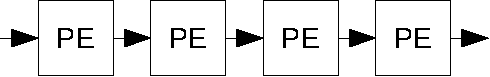
\includegraphics[scale=.5]{images/pipeline.pdf}
    \vspace*{1.15cm}
    \caption[]%
    {{\small Pipeline}}
    \label{fig:pipeline}
  \end{subfigure}
  %\hspace*{\fill}
  \begin{subfigure}[b]{0.475\textwidth}
    \centering
    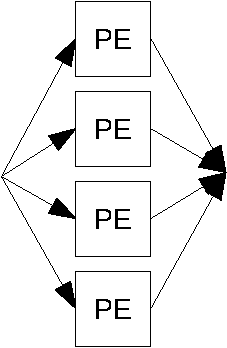
\includegraphics[scale=.5]{images/parallel.pdf}
    \caption[]%
    {{\small Parallel}}
    \label{fig:parallel}
  \end{subfigure}
  \vskip\baselineskip
  \begin{subfigure}[b]{0.475\textwidth}
    \centering
    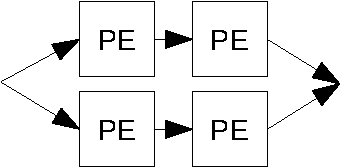
\includegraphics[scale=.5]{images/parallel-pipeline.pdf}
    \caption[]%
    {{\small Parallel pipeline}}
    \label{fig:parallel-pipeline}
  \end{subfigure}
  %\hspace*{\fill}
  \begin{subfigure}[b]{0.475\textwidth}
    \centering
    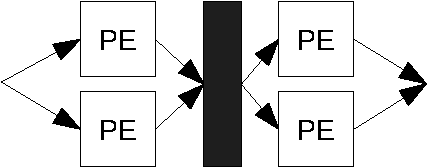
\includegraphics[scale=.5]{images/pipeline-parallel.pdf}
    \caption[]%
    {{\small Pipeline of parallel}}
    \label{fig:pipeline-parallel}
  \end{subfigure}
  \caption[]
  {\small Different processing element architectures}
  \label{fig:processing-element-organization}
\end{figure*}

The parallel configuration is typically used for higher layer networking applications, where as the pipeline configurations are used in line cards that require high-speed processing at low layer networking applications.

\section{Programming Models}

% \todo[inline]{Write a general view of the NPU programming models.}

Several generic software, development, and have been proposed to ease the development of high-speed packet processing applications for network processors.

% Different frameworks, such as Data Plane Development Kit~\cite{Intel:DPDK}, Open vSwitch~\cite{Pfaff:2009:OVS}, and Open Event Machine~\cite{OpenEM}, have been implemented to

\subsection{Data Plane Development Kit}
The Data Plane Development Kit (DPDK) provides a clean application programming interface and a set of coherent libraries and drivers, for Intel x86 processors. It has a generic support for many CPU's and network interface controllers ranging from Intel Atom processors to Intel Xeon processors. It supports system with and without non-uniform memory access (NUMA), and any number of processing cores.~\cite{Intel:DPDK:Doc}

DPDK runs as a Linux user-space application, utilizing the pthread library. Similarly to many other packet processing frameworks, DPDK implements a run-to-completion model, to minimize the process-switching overhead. The model removes the typical operating system scheduler. All the devices must be accessed by polling, thus eliminating the interrupt overhead. The packets can be passed between the cores, enabling more efficient and flexible core usage.~\cite{Intel:DPDK:Doc}

DPDK's Environment Abstraction Layer (EAL) abstracts the hardware environment from applications and libraries, enabling hardware agnostic implementation of packet processing applications. EAL provides services such as core affinity and assignment procedures, memory management, atomic and lock operations, and bus accesses, and interrupt handling. These features are exposed as a programming libraries.~\cite{Intel:DPDK:Doc}

DPDK has an active ecosystem around it, with wide vendor support. It is also well documented and includes several software examples demonstrating the best practices for data plane architectures, application profiling, and performance tuning.~\cite{Intel:DPDK:Doc}

\subsection{Open Event-Machine}
Open Event Machine (OpenEM) is an event-driven programming framework for multicore dataplane applications, developed by Nokia Solutions and Networks (NSN). It has been designed to ease the implementation of event/packet processing applications for different MPSoC devices. One of main drivers for the development of OpenEM has been easy integration with modern hardware accelerators.

The key concepts of OpenEM framework are execution objects, events, queues, and the scheduler. \emph{Execution objects} are the main building blocks the OpenEM application. They are the run-to-completion functions, describing the processing logic of the application. Each execution object has one or more \emph{queues} attached to it. The \emph{scheduler} selects the events from the queues, based on the global interrelations of the queues. When the event is selected from the queue, the corresponding execution object is attached to the processing core, and the event is passed to it as a parameter. Once the execution object finishes its run, the scheduler chooses a new event from the queues similarly.

From the programmer's perspective, OpenEM's event-driven programming model relates closely to actor based programming models such as Erlang~\cite{Armstrong:1993:Concurrent} and Akka framework~\cite{Akka}. While the use cases for these frameworks are completely different, and thus cannot directly be compared with OpenEM, it is worth mentioning their message passing support. Support for combined inter-node and intra-node parallelism has potential benefits for efficient scaling in the future. HCMPI~\cite{Chatterjee:2013:HCMPI} is an example of experimental framework that combines task-parallelism with message passing. OpenEM's current specification does not support inter-node messaging.

\section{Cavium OCTEON II CN6880}
\label{sec:cavium-octeon}
%https://www.reddit.com/r/networking/comments/2kamp1/eli5_why_are_cavium_chipsets_so_popular_with
Cavium Octeon II CN6880 is a network processing unit, optimized for high-performance, high-bandwidth, and low power consumption software-defined control-plane and data-plane applications.

CN6880's ingress and egress processing are handled by separate processing elements. The packet input processor unit (PKI) and input packet data unit (IPD) work together to manage the received packets, and to perform required processing before scheduling the packets to application cores. Once the required ingress computation is done, the PKI unit sends the packet's work entry to the SSO unit to be scheduled for processing.~\cite{cavium:2010:fundamentals}

The egress functions are handled by the packet transmission unit (PKO). When a core finishes a packet processing, it notifies the PKO that the packet is ready for transmission. The PKO then directly copies the packet data from the shared memory into its internal memory, optionally computes checksums for the packet header, transmits the packet, and optionally frees the packet data from the memory.~\cite{cavium:2010:fundamentals}

CN6880 consists of 32 MIPS application cores, with several hardware acceleration units for enhanced packet processing and minimized software development complexity. The packet management accelerators offload the actual packet processing cores from many general packet receive, buffering, buffer management, flow classification, quality of service, and transmit processing. The accelerator functions can be customized using software, and accessing the configuration registers. Together with the hardware acceleration units, the processing cores can handle most of the processing requirements of all the way through layer 2 to layer 7 in the standard OSI model~\cite{ISO:1994:OSI}.~\cite{cavium:2010:fundamentals}

One of the key features of the CN6880 is its scheduling/synchronization and order unit (SSO). It frees the actual packet processing applications, running on the 32 MIPS cores, from the complex packet scheduling and ordering tasks. The cores execute a loop, and when a core is ready for the next packet, it requests work from the SSO, which then schedules the next work based on the quality of service priority and work group.~\cite{cavium:2010:fundamentals}

The SSO has efficient locking mechanisms for protecting the critical regions without explicit software locking, and allows packet processing to be done in parallel or atomically, while still maintaining the packet flow order. The processing cores can also be dedicated for specific flows. One of our goals is to be able to model the scheduling functionality with PSE, as it is one of the key elements in the packet latency and throughput when processing several flows at the time.~\cite{cavium:2010:fundamentals}

% The memory latencies have large effect in the packet processing times.

The CN6880 provides several memory policies for optimized multi-core packet processing. Each of the 32 cores have dedicated 32KB L1 data and 37KB L1 instruction cache, and a shared 4MB L2 cache. The L1 data cache provides a hybrid write-through, write-back policy, using a write buffer mechanism, and the L2 cache implements a write-back policy. Several other cache related features are offered, for example to avoid unnecessary data writes after the packet transmission, and to automatically send the received packet header to L2 cache and the packet data to main memory, bypassing the L2 cache.~\cite{cavium:2010:fundamentals}

\section{Characteristic Measurements}
\label{sec:characteristic-measurements}

For the model to represent the packet latencies and throughput with enough accuracy, the model needs to be filled with apposite entity parameters. Some of the model parameters are simple enough to be obtained directly from~\cite{cavium:2010:fundamentals}, while others are either unavailable, or are presented in an unusable form to be used in the simulation model. The missing communication and memory related parameters are obtained by conducting measurements on the real CN6880 hardware. These are discussed in the following sections, respectively.

% We believe that, by determining the latecies of input phase and output phase, the behavior of memory, and modeling the packet scheduler with enough accuracy, the sought applications' effects to the packet latencies and throughput come up with enough accuracy.

% For our approach to be valid, i.e. the abstraction of the communication latencies to be precise enough, we have to assume the fastpath is not the bottleneck in the processing phase. This assumption is reasonable because ...

% \fixme{
%   TODO:
%   \begin{itemize}
%   \item because the fastpath hardware is optimized for this task
%   \item find reference
%   \item maybe justify the stuff with some kind of rough back-of-the-envelope calculation?
%   \end{itemize}
% }

\subsection{Communication Latencies}
\label{sec:communication-latencies}

By communication latencies, we refer to the time in the input and output phase of the packet processing, between physical receive/transmit ports and the actual core processing, as described in the Section~\ref{sec:cavium-octeon}. We will include the times spent in the SSO unit for both of these metrics, as due to our resource constraints, we were unable to do the measurements with the required detail to break down these delays. Also, for our modeling purposes, it is accurate enough to assume that the input and output phases consume equal amount of processing time.

The input and output phase latencies are measured by generating traffic from external machine, and passing it through two CN6880 units back to the generator itself. The measurements were done at two independent points in the processing path, to validate the accuracy of the measurements.

\begin{figure}[]
  \begin{center}
    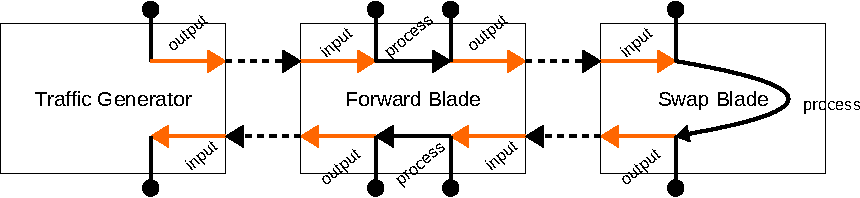
\includegraphics[width=\textwidth]{images/comm-measurement-setup.pdf}
    \caption{The setup used to measure the communication latencies. The communication between the nodes, packet processing on the main cores, and the input and output processing, are marked with the dashed arrows, solid black arrows, and orange arrows respectively. The probes present the points of measurement.}
    \label{fig:comm-setup}
  \end{center}
\end{figure}

In Figure~\ref{fig:comm-setup}, the rectangles represent three different computing units (traffic generator, forward unit, and swap unit), and the probes present the points of time measurements. The traffic generator is a typical desktop computer running Ubuntu operating system, and the traffic was generated by Mausezahn~\cite{mausezahn}. Both of the Octeon CN6880 units are running Linux operating systems.

The packet is first generated at the packet generator and sent to the forward unit at time $t^{d}_{0}$. Forwarding unit receives the packet at time $t^{r}_{10}$, does the required processing and forwards the packet to the swap unit at time $t^{d}_{10}$. The swap unit receives the packet at time $t^{r}_{2}$, does the same processing as the forward unit (except with different destination address), and forwards the packet back to the forward unit at time $t^{d}_{2}$. Finally the forward unit receives the packet at time $t^{r}_{11}$ and forwards it to the traffic generator at time $t^{d}_{11}$, which marks it received at time $t^{r}_{0}$. The time $t_{f}$ spent in the input and output phase of one unit is then

\begin{equation}
  \label{eq:1}
  t_{f} \approx \frac{t^{r}_{11} - t^{d}_{10} - (t^{d}_{2} - t^{r}_{2})}{2}.
\end{equation}

We measured the times for packet sizes of 64B, 128B, 256B, 512B, 1024B, and 1500B, repeating the measurement for each packet 10000 times. Figures~\ref{fig:comm-latency-boxplot} and~\ref{fig:comm-latency-histograms} present the statistics of the resulting times $t_{f}$ for the different packet sizes.

\begin{figure}[]
  \begin{center}
    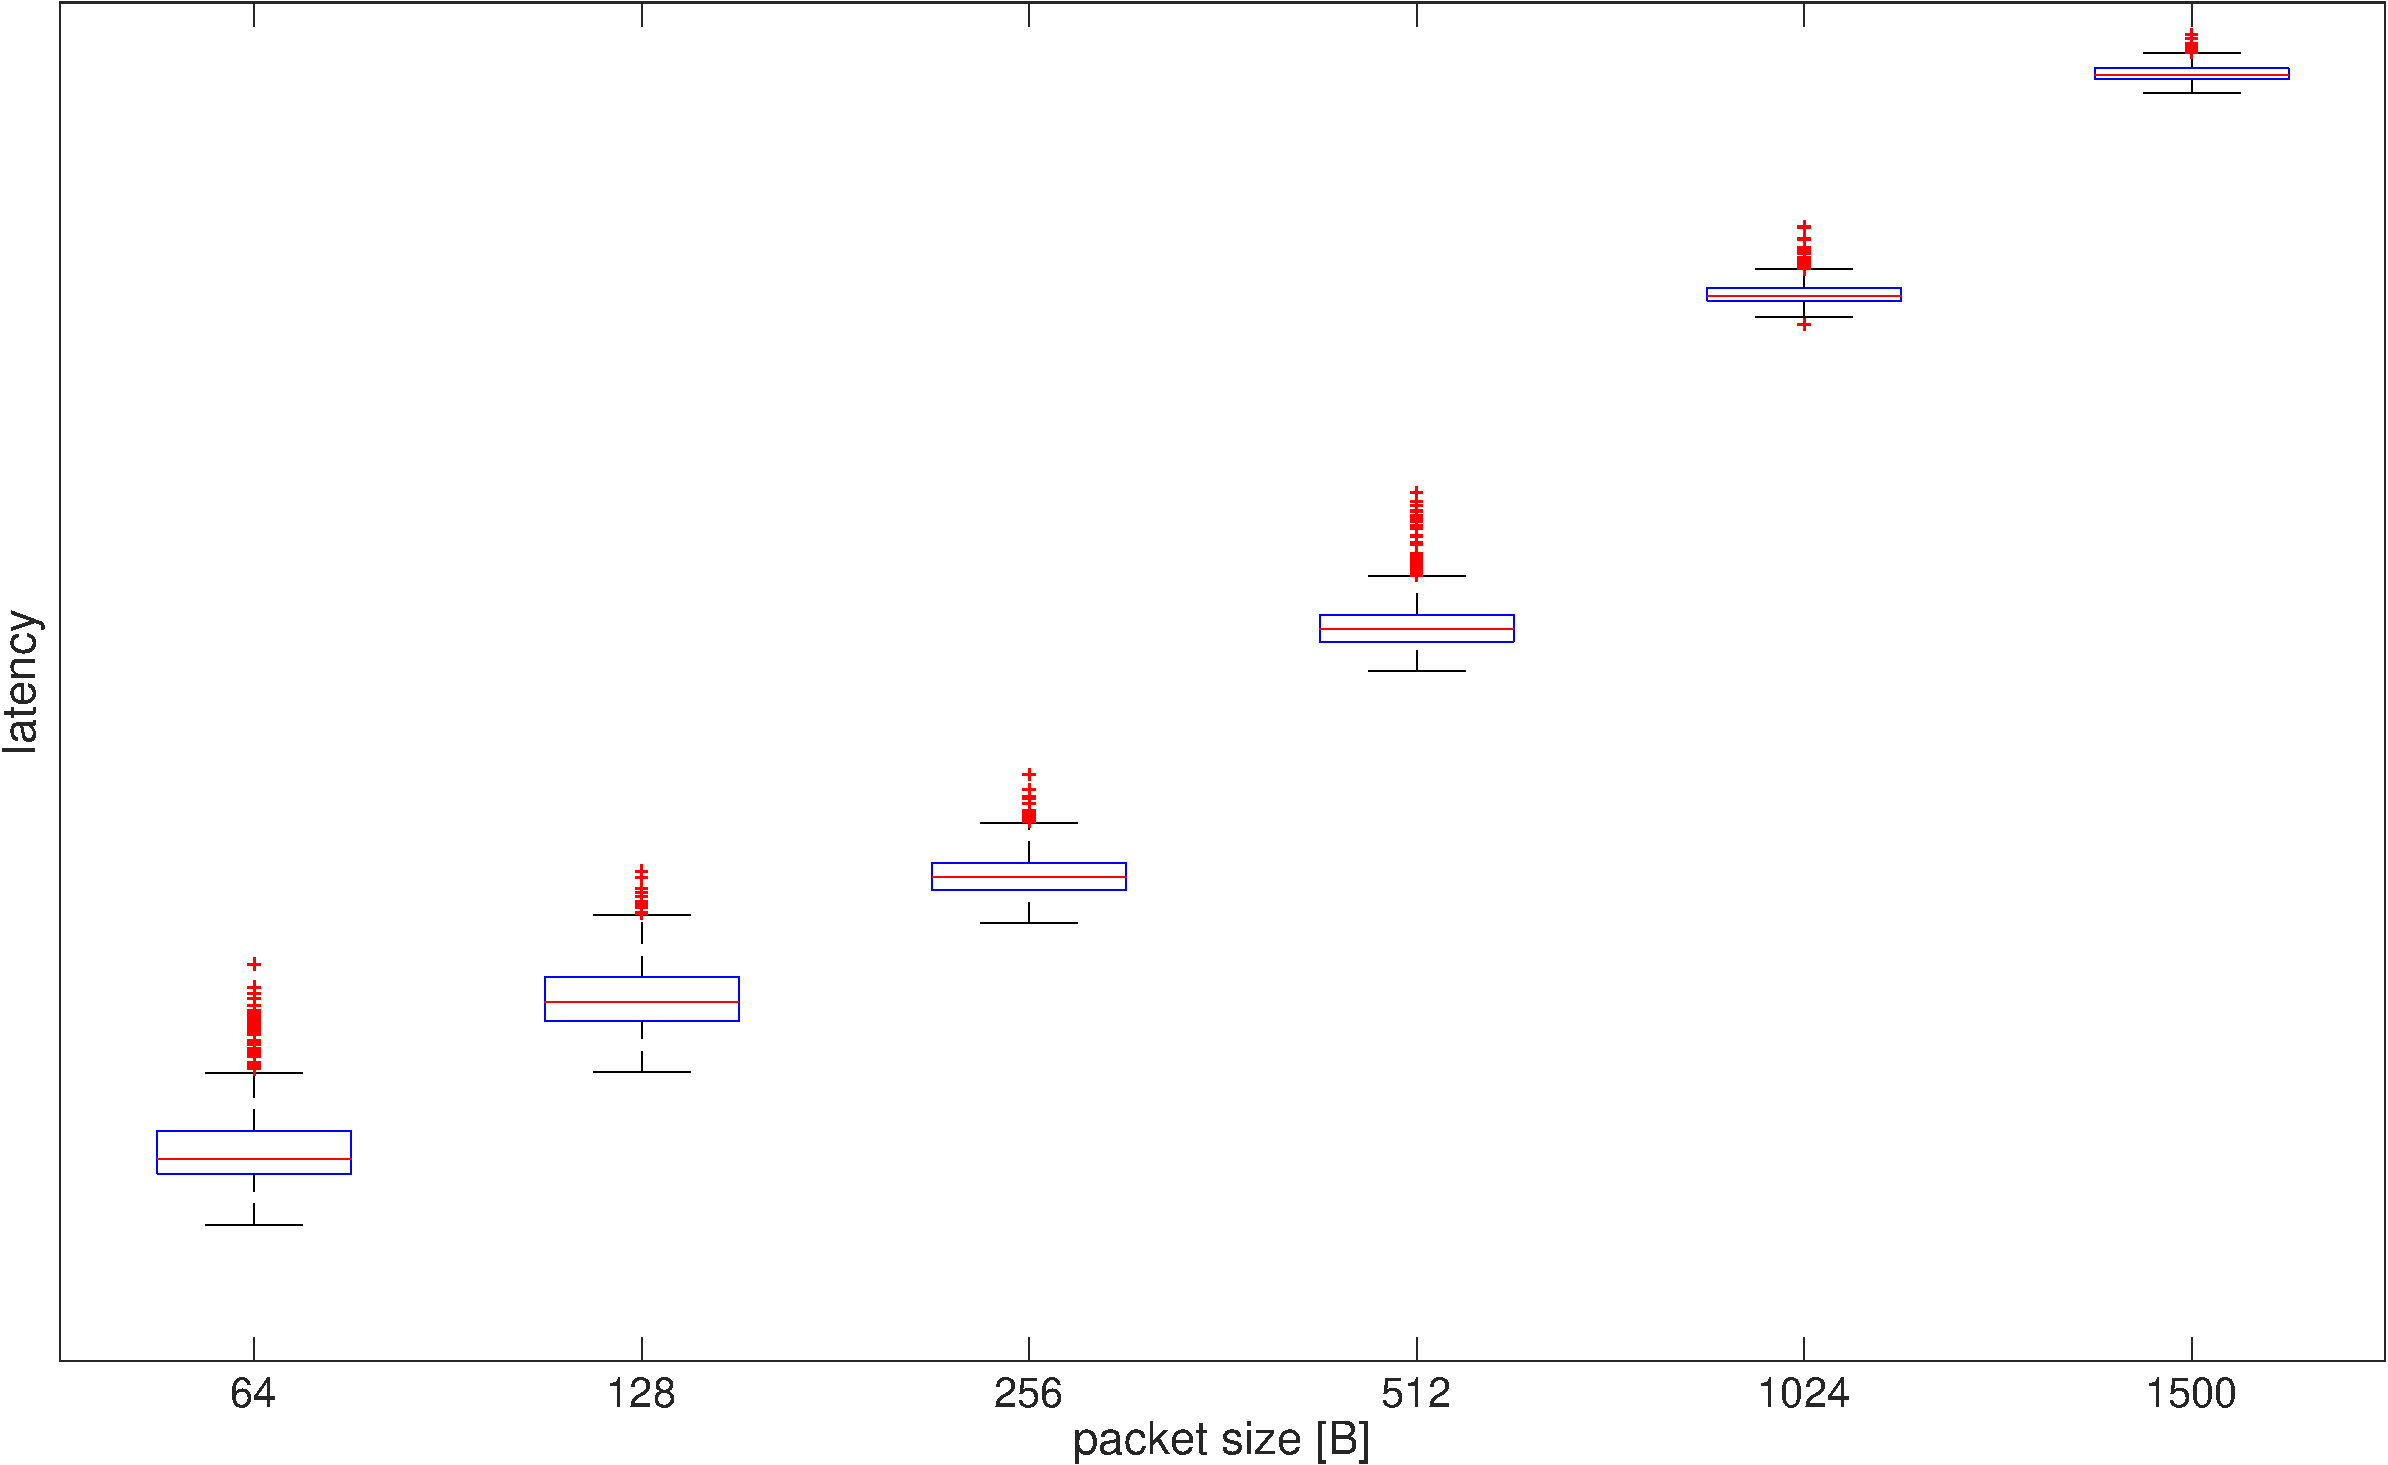
\includegraphics[width=\textwidth]{images/comm-latency-boxplot.pdf}
    \caption{Latency of the input and output phase of the CN6880 unit. On each box, the central mark is the median, the edges of the box are the 25th and 75th percentiles. 99.3\% of the points lie within the whiskers, and the most extreme points are presented as red crosses. Both of the axes are on logarithmic scale.}
    \label{fig:comm-latency-boxplot}
  \end{center}
\end{figure}

\begin{figure}[]
  \begin{center}
    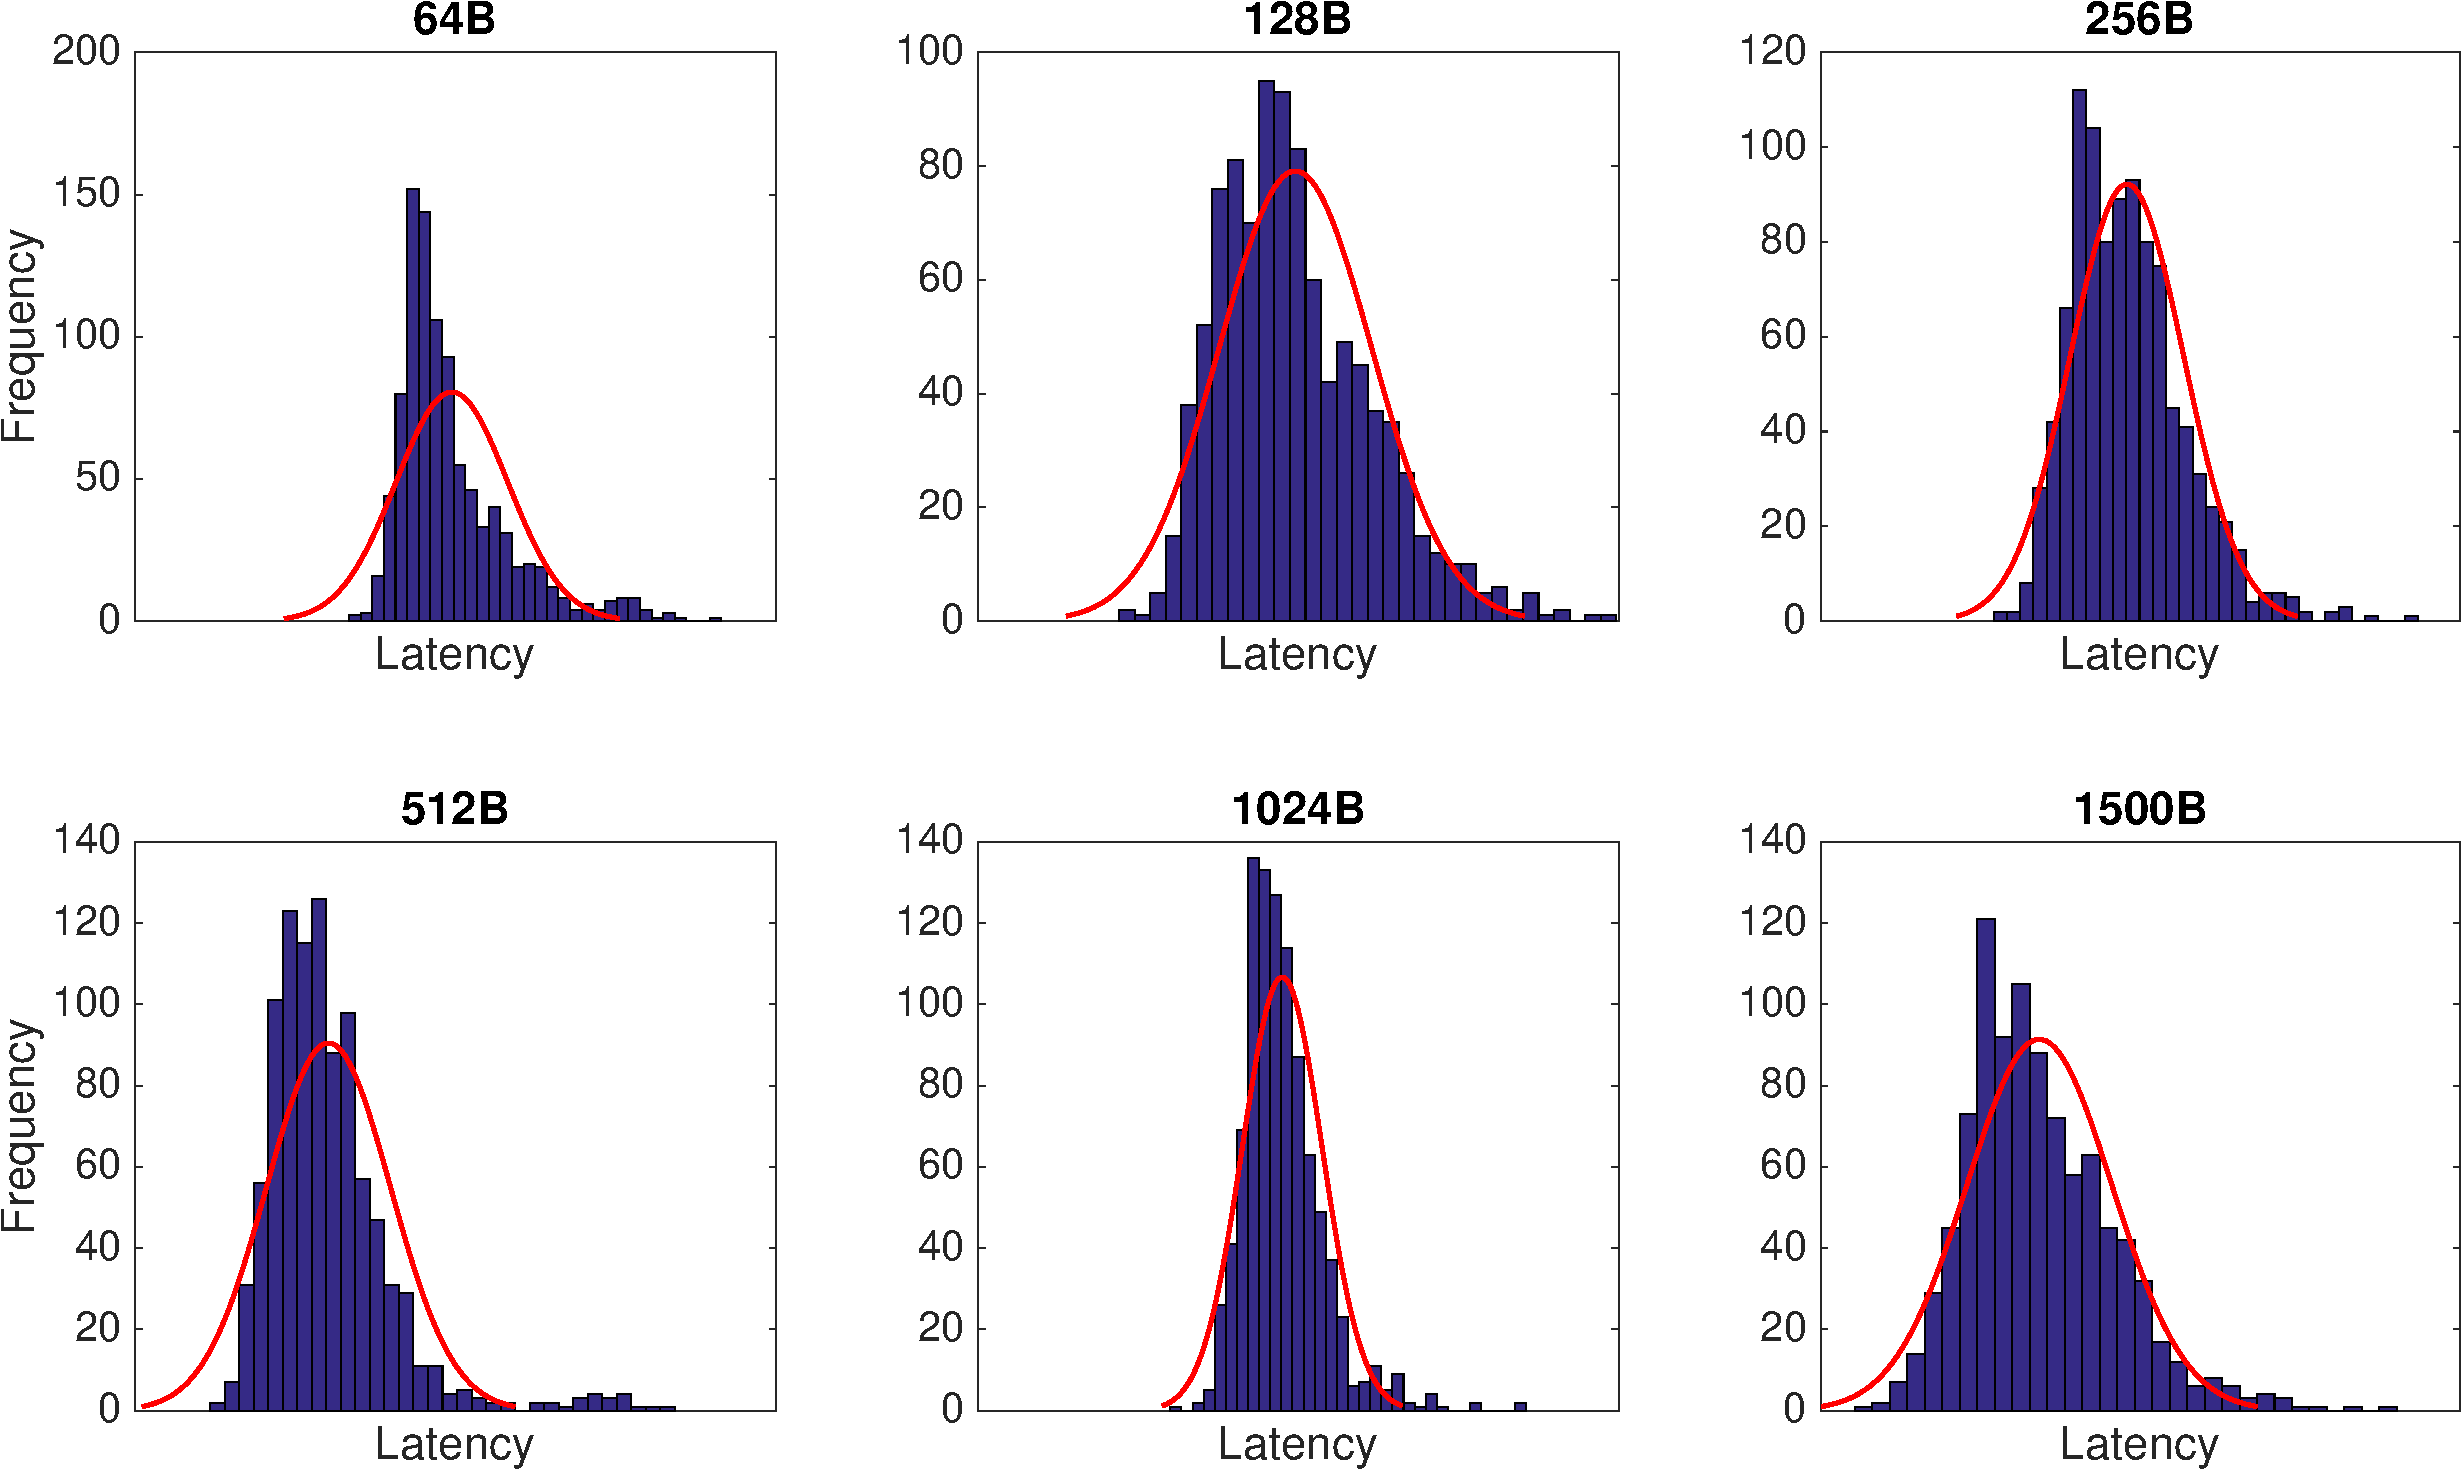
\includegraphics[width=\textwidth]{images/comm-latency-histograms.pdf}
    \caption{Latency frequency histograms for each packet size, along with a normal density function with parameters, estimated with maximum likelihood method from the data.}
    \label{fig:comm-latency-histograms}
  \end{center}
\end{figure}

As shown in the Figure~\ref{fig:comm-latency-boxplot}, the time spent in the input and output phase of the unit is roughly linear regarding to the packet size. The variation of the data is relatively small on all packet sizes. The trend of the latency with respect to the packet size, corresponds to the trend of the values measured with at the external traffic-generator (which causes $3.1\mu s$ constant overhead regardless of the packet size). The corresponding plots for the external traffic-generator measurements are omitted for clarity.

As seen from both of the Figures~\ref{fig:comm-latency-boxplot} and ~\ref{fig:comm-latency-histograms}, there exist points with unexpectly large deviation from the rest of the group. These deviations seem to be independent of the packet size, and thus we assume that they are caused by the scheduling unit (SSO). This behavior is also statistically incorporated in the simulation model.

The only packet size dependent operations in the input and output phases are the memory transfers done for the actual packet data between the memory (L2/RAM) and PKI or PKO. All the other other operations are done based on the packet header, thus requiring constant amount of time regardless of the packet size.

Since We cannot make a distinction between the input and output phase, in the simulation model presented further, we will adjust the input/output phase amount so that they consume the PKI and PKO units for the amount that corresponds the constant term of equation~\ref{eq:1}. The variable (non-constant) term is caused by the memory copies in the input/output phases, and are proportional to the packet size.

The input and output delays used in the simulation model are estimated by fitting a linear model to the data, using least square estimate. The determination coefficient of the estimate $R^2 = 0.997$. The delay for the input and output phase are divided evenly, resulting in

\begin{equation}
  \label{eq:1}
  t_{in} = t_{out} = \frac{1}{2}(0.0018\frac{\mu s}{B} * packet\_size + 1.036\mu s).
\end{equation}

\subsection{Memory Characteristics}
\label{sec:memory-characteristics}

Memory delays were measured using Multi-core Processor Architecture and Communication (MPAC) benchmarking library~\cite{Jamal:2009:MPAC}. Both, latency and throughput were measured using different dataset sizes and number of threads. Each the tests was run with 200,000 repetitions.

\begin{figure}[]
  \begin{center}
    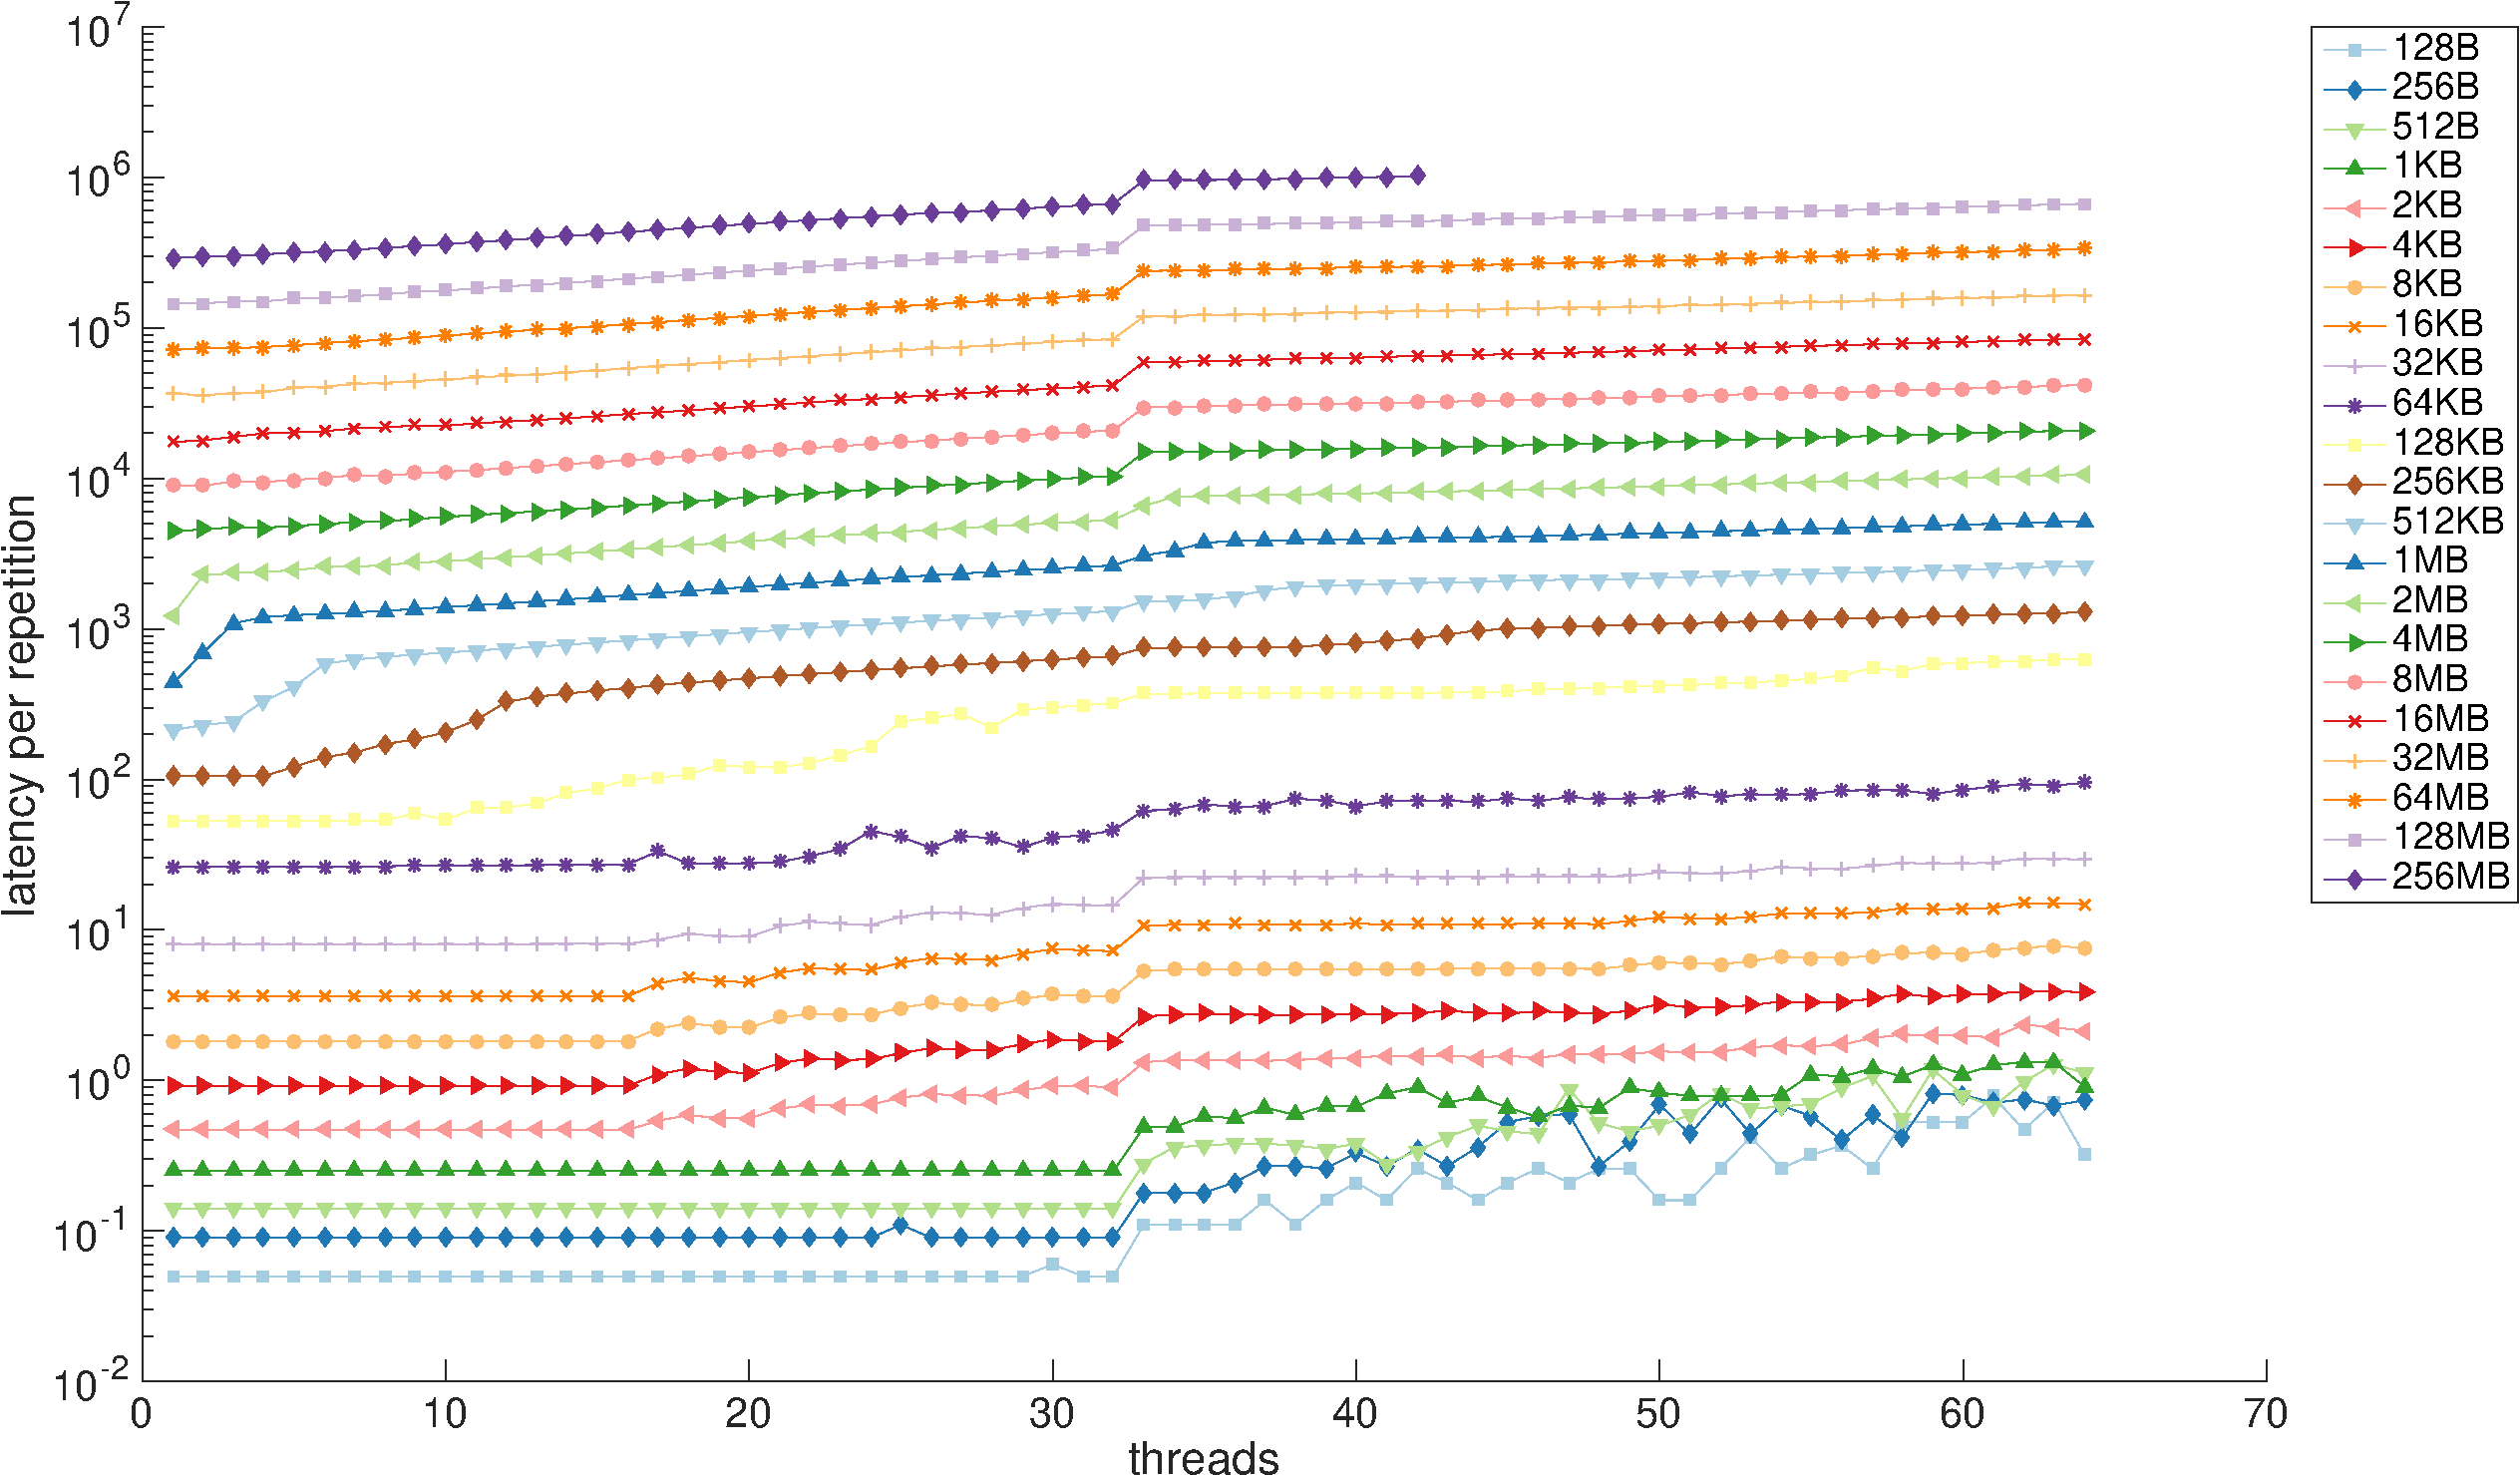
\includegraphics[width=\textwidth]{images/mem-latency.pdf}
    \caption{Memory latency of the CN6880 in microseconds across number of threads for integer data type (32bit), measured by MPAC. Each data point in the graph present one experiment run with different thread and write sizes. The latencies for different packet sizes are marked with colors as shown in the legend (in bytes). The y-axis is presented in logarithmic scale.}
    \label{fig:mem-latency}
  \end{center}
\end{figure}

Figure~\ref{fig:mem-latency} presents the results from the latency measurements for different packet sizes and thread counts. Notice that the y-axis the graph is logarithmic. As expected, the memory latencies grow together with the size of the write. The transition between the memory levels (32K L1, 4MB L2~\cite{cavium:2010:fundamentals}) can be seen as the jumps in the latency graph. With 128B - 1KB write sizes both the read and write arrays fit in the L1 cache (32KB~\cite{cavium:2010:fundamentals}), and thus the latency per repetition is independent of the thread count. With write sizes above 2KB, some of the writes hit L2 cache (4MB~\cite{cavium:2010:fundamentals}), increasing the latency as the thread count increases. Similarly, the step from L2 cache to RAM can be seen 128KB, 256KB, 512KB, 1MB, and 2MB write sizes, where both write and read arrays completely fit in the L2 cache with 8, 4, 2, 1 and 1 threads, and move to RAM beyond that.

The write latencies also thrash beyond 32 threads, especially for the cache sizes. This does not affect the main core memory accesses in the model, as only 32 threads are used for packet processing. However, these numbers work as a reference when modeling the memory communication of other units such as SSO.

\begin{figure}[]
  \begin{center}
    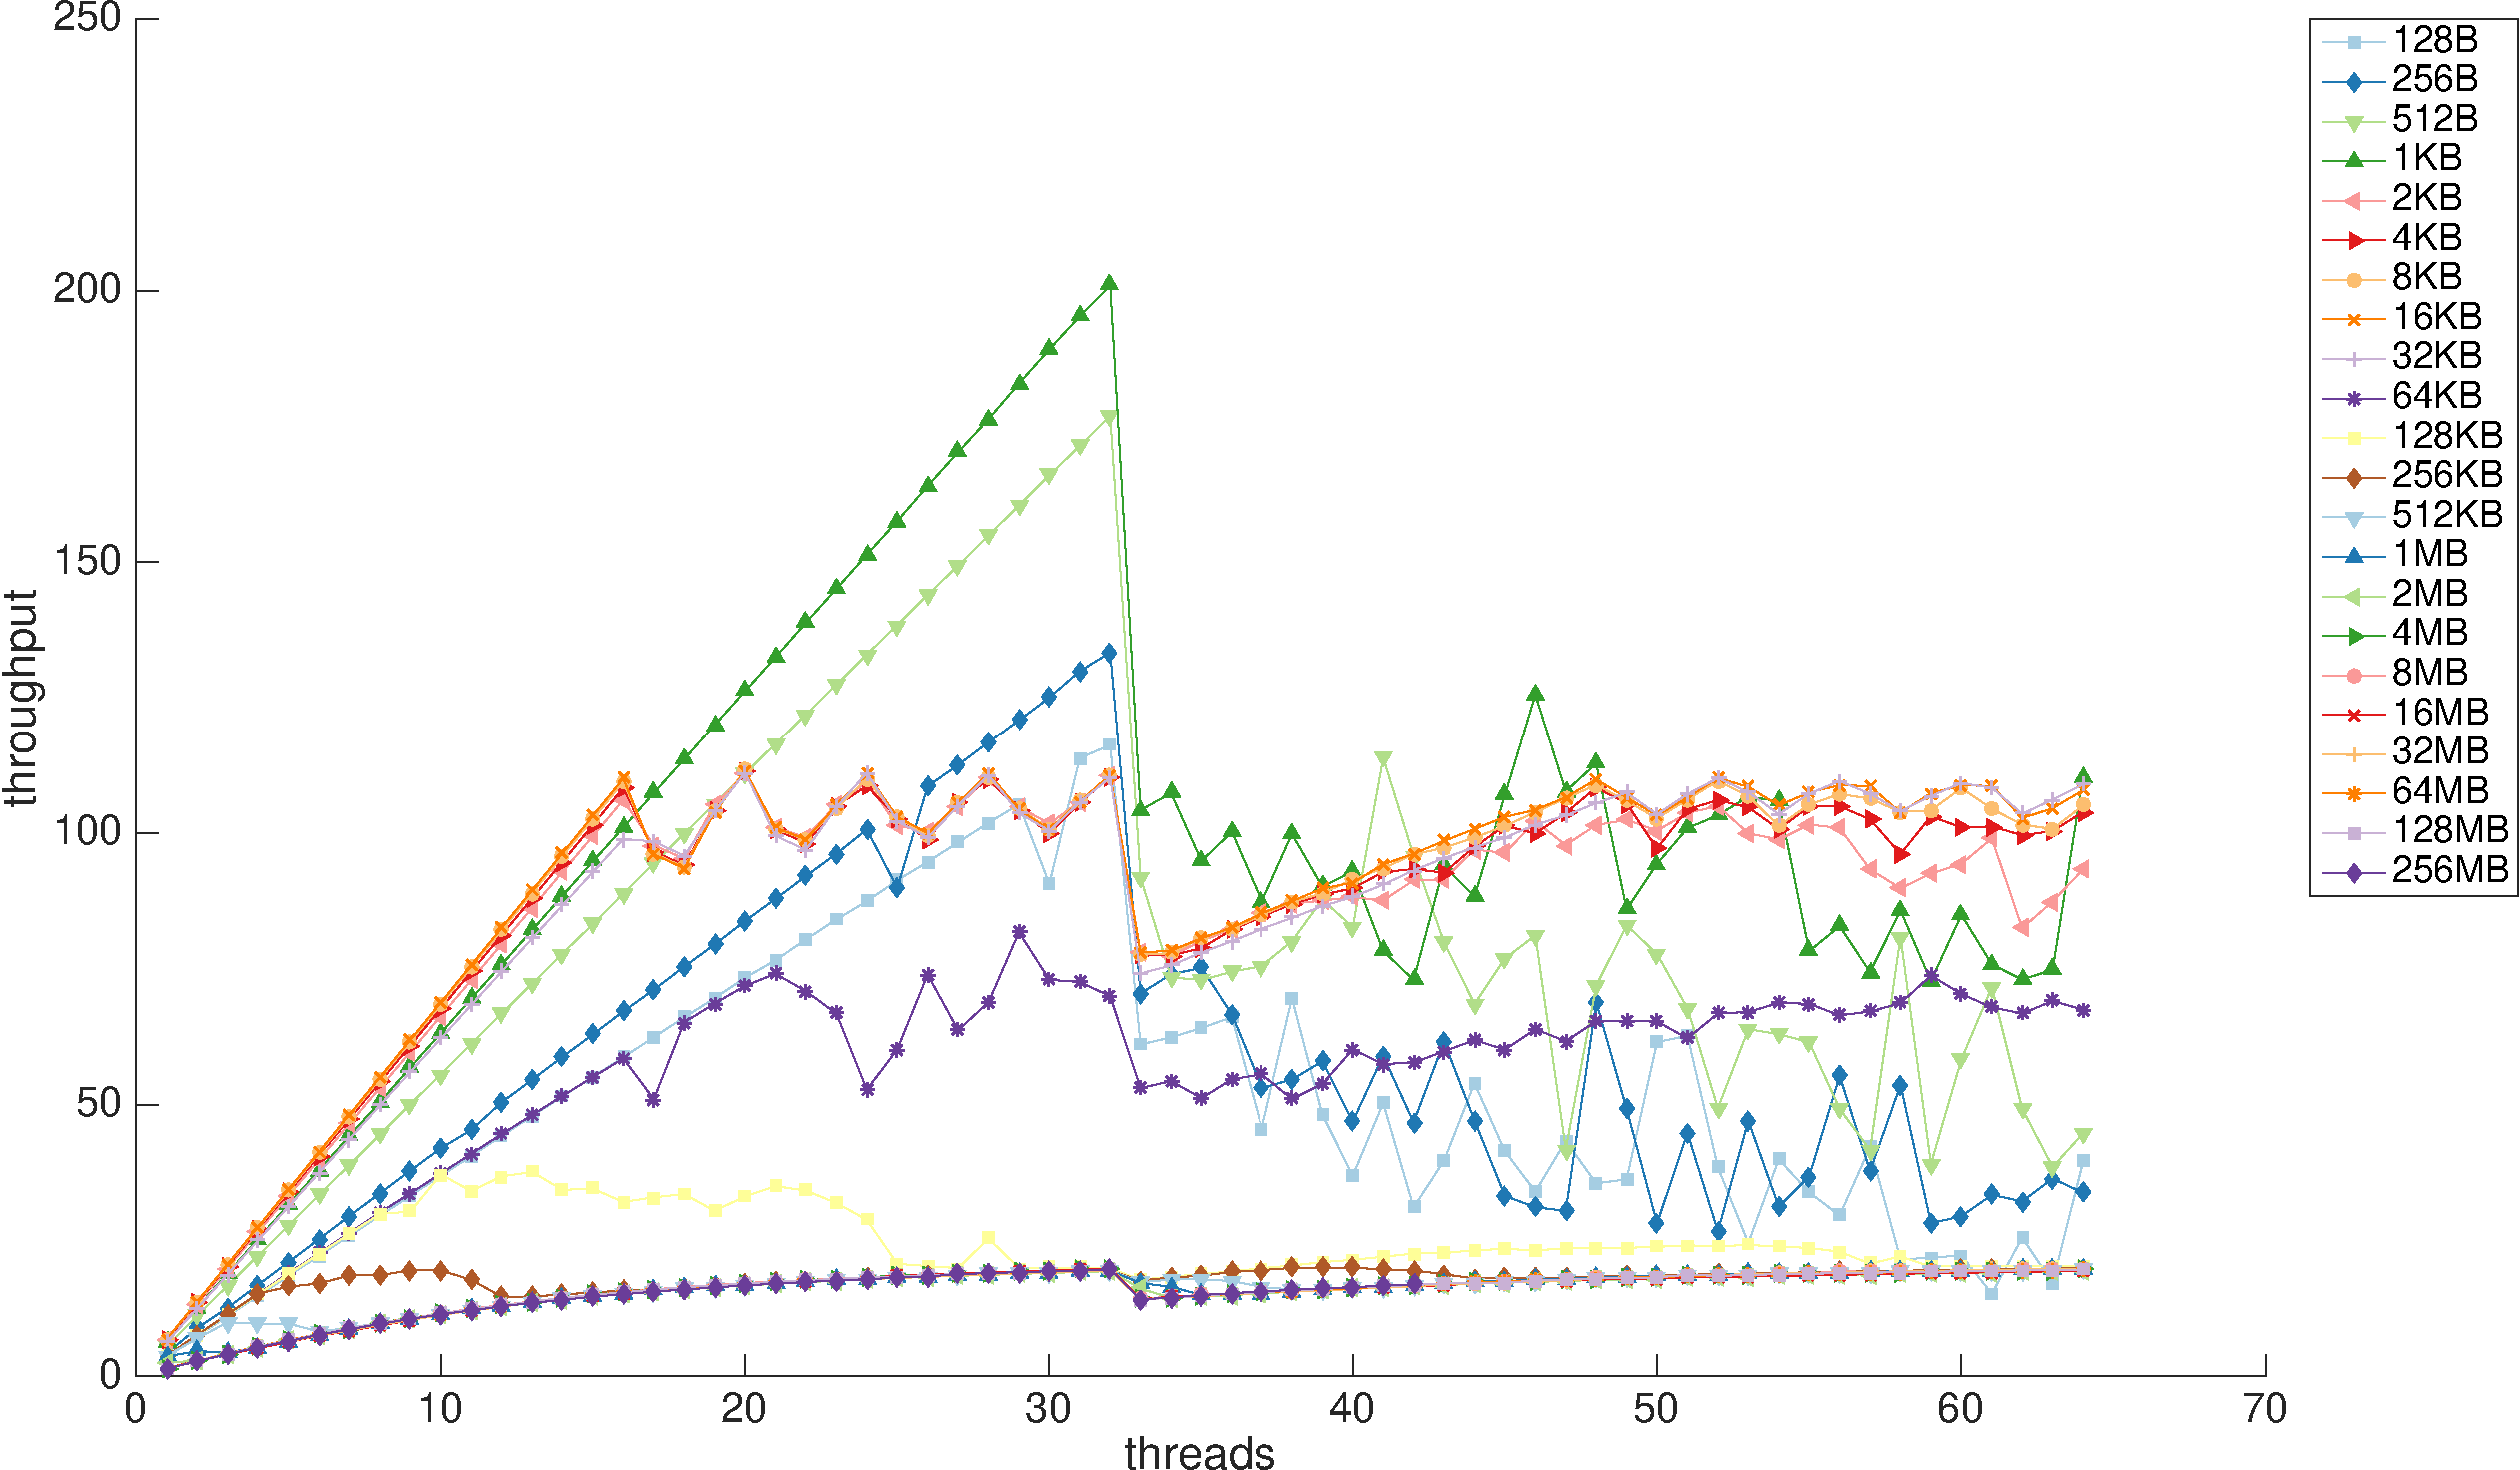
\includegraphics[width=\textwidth]{images/mem-throughput.pdf}
    \caption{Memory throughput of the CN6880 in Gbps across number of threads for integer data type (32bit), measured by MPAC. Each data point in the graph present one experiment run with different thread and data sizes. The throughput for different packet sizes are marked with colors as shown in the legend (in bytes).}
    \label{fig:mem-throughput}
  \end{center}
\end{figure}

Figure~\ref{fig:mem-latency} presents the results from the throughput measurements for different packet sizes and thread counts. Again, as expected, the maximum throughput is achieved with 1KB write lengths and 32 cores, when both the write and read arrays fit in the caches. The write throughput scales linearly with 128B - 1KB write sizes for up to 32 cores, with 2KB - 64KB up to 16 cores, and for 256KB, 512KB, and 1MB, write sizes up to 8, 4, and 2 cores respectively. The transitions between the memory levels are similar as in the latency graph. Again, a clear thrashing can be seen with more than 32 threads.


%%% Local Variables:
%%% mode: latex
%%% TeX-master: "thesis-hartikainen"
%%% End:

\chapter{Mechanism For Extended Queue Disciplines}
\label{chapter:mechanism-for-extended-queue-disciplines}

This chapter presents the implemented plugin code extensions for Performance Simulation Environment. The extensions enable modeling of customized queue disciplines written in C-code, and is our attempt to address the lack of global queue scheduling, which is required to use PSE for more detailed modeling of hardware scheduled manycore systems.

We begin by explaining the PSE's service routines, which guide the resource usage between the resource usage and resource provision models. Then we present the runtime structuces, RNS\_Resource and RNS\_Client, that are relevant to understand the implementation of the custom queueing functions. Then we present the requirements for the select and reserve functions used to implement the queuing policies. Finally, we describe an example implementations of two simple disciplines: first-come-first-serve and highest-priority-served-first.

\section{Service Routines}
The main interface between the threads executing the resource usage code, and the resource provision models, are the five RNS service routines: RNS\_demand\_device, RNS\_use\_device, RNS\_reserve\_resource, RNS\_delay\_process, and RNS\_release\_resource. The functions are used to implement both the active and passive resource usage at the runtime.

\lstinputlisting[caption=RNS\_demand\_device,
                 label=lst:RNS-demand-device]{listings/RNS_demand_device.c}

RNS\_demand\_device routine in Listing~\ref{lst:RNS-demand-device} is a simple wrapper routine, which converts the demanded service amount (service\_amount) into corresponding service time, based on the device entity speed (d-$\textgreater$speed). It then calls the RNS\_use\_device routine with the resulting service time.

\lstinputlisting[caption=RNS\_use\_device,
                 label=lst:RNS-use-device]{listings/RNS_use_device.c}

RNS\_use\_device in Listing~\ref{lst:RNS-use-device} reserves the resource, delays the process (i.e. the task) and immediately releases the resource for other processes.

\lstinputlisting[caption=RNS\_reserve\_resource,
                 label=lst:RNS-reserve-resource]{listings/RNS_reserve_resource.c}

Listing~\ref{lst:RNS-reserve-resource} summarizes the RNS\_reserve\_resource routine. Whenever the process executing the resource usage code consumes a resource (passive or active), the RNS\_reserve\_resource -function gets called. In the case of passive resource, the call happens directly in the generated resource usage code. If the requested resource is active, the RNS\_reserve\_resource call happens through the RNS\_use\_device or RNS\_demand\_device functions.

RNS\_reserve\_resource calls the reserve function bound to the resource entity as explained further. The reserve function assigns the task either to the resource's processing queue or waiting queue. If the reserve function assigns the task to the waiting queue, the thread yields the execution back to the scheduler.

\lstinputlisting[caption=RNS\_delay\_process,
                 label=lst:RNS-delay-process]{listings/RNS_delay_process.c}

RNS\_delay\_process function, presented in Listing~\ref{lst:RNS-reserve-resource}, delays the given process for the time defined by the \emph{seconds} parameter and generates an event that will be triggered when the requested service has ended.

\lstinputlisting[caption=RNS\_release\_resource,
                 label=lst:RNS-release-resource]{listings/RNS_release_resource.c}

RNS\_release\_resource function, shown in ~\ref{lst:RNS-reserve-resource}, selects the next process to be executed from the resource queue, based on the resource's queue discipline function. The selected process is inserted in to the heap of schedulable processes, and thus gets immediately scheduled.

\section{Runtime Structures}
\subsection{RNS Resource}
Each resource entity in the PSE resource provision model definition corresponds to a RNS\_Resource runtime variable. The runtime resources are initialized in the beginning of the simulation, based on the code generated from the resource provision entity. Listing~\ref{lst:RNS-Resource} presents the RNS\_Resource struct.

\lstinputlisting[caption=RNS\_Resource struct. ,
                 label=lst:RNS-Resource]{listings/RNS_Resource.c}

The \emph{id} is a unique identifier for the resource, determined by the RNS runtime. The \emph{name}, \emph{capacity}, and \emph{group\_name} are defined by the attributes in the model entity. The \emph{probes} array contains the references to the probe structs attached to the resource entity.

The \emph{processing\_queue}, and the \emph{waiting\_queue} present the data structures used to store the references to the clients that are being processed by and waiting for the resource, respectively. The size of the processing queue is determined, at runtime, by the \emph{capacity} parameter defined in the resource provision model. The size of the waiting queue is fixed, defined by the built-in \emph{RNS\_LARGE} constant. \emph{processing\_count} and \emph{waiting\_count} are initialized to 0, and present the number of clients in the respective queues.

The two function pointers, \emph{select} and \emph{reserve}, are the actual functions used to implement the queue disciplines for the resource. The values of these pointers are determined by the \emph{discipline}, \emph{file}, \emph{select\_function}, and \emph{reserve\_function} in the resource entity's attributes.

The possible values for \emph{discipline} attribute are: \emph{CUSTOM}, to use custom disciplines determined in the external plugin files; or one of \emph{FCFS}, \emph{LCFS}, \emph{HPSF}, \emph{LRSF}, to use the built-in disciplines. If the discipline attribute is set to use the built-in disciplines, the model entity's \emph{file}, \emph{select\_function}, and \emph{reserve\_function} can be left blank, and the corrent pointers for the \emph{select} and \emph{reserve} functions are set automatically.

If the discipline is set to CUSTOM, then the pointers to the discipline functions are set to the functions named by the values of \emph{select\_function} and \emph{reserve\_function} paramaters found in the file named by the \emph{file} parameter.

\subsection{RNS Client}
RNS\_Client is the runtime representation of the task consuming a resource. The RNS\_Client struct is shown in the Listing~\ref{lst:RNS-Client}. The \emph{process} field is a pointer to the RNS\_process that reserved the resource. \emph{usage\_group} is used for trace probe grouping, and \emph{pc} is the old priority attribute left here for the backwards compatibility. In the current version of PSE, the priority should be specified in the \emph{attrs} field, together with all the other attributes to be used in the select and reserve functions. The \emph{processing} parameter specifies whether the client is currently being processed or not.

\lstinputlisting[caption=RNS\_Client struct. ,
                 label=lst:RNS-Client]{listings/RNS_Client.c}

Each time a process reserves resource, the corresponing RNS\_Client entity's \emph{attrs} field, at the RNS\_Resource's processing or waiting queue, is set to the values described by the node in the resource usage model. The \emph{RNS\_Queue\_Attribute} fields are determined in the compile time, based on the attributes determined in the resource usage model's nodes.

\section{Reserve and Select Functions}

As explained above, the queue discipline functionality is determined by the two functions: the reserve function and the selection function. These two functions must follow certain rules and definitions to guarantee the proper scheduling and simulation behavior. The definition of the reserve and select functions are shown in the Listings~\ref{lst:reserve-definition} and~\ref{lst:select-definition}, respectively.

\lstinputlisting[caption=The definition of the reserve function. ,
                 label=lst:reserve-definition]{listings/reserve_definition.c}

The reserve function is called from the RNS\_reserve\_resource function when the task requests  the resource for the first time. The parameter \emph{r} represents the requested resource entity, and the \emph{new\_client} is the client requesting for the resource. The reserve function needs to perform the following tasks:

\begin{itemize}
\item Set the \emph{queue} to point to either the processing queue or the waiting queue of the resource \emph{r}
\item Assign an integer to the \emph{position}, presenting an empty position in the queue
\item (Optionally) reorganize the waiting queue
\item Return 0 in case of success, else return -1
\end{itemize}

All the necessary information required to implement the queueing decision can be accessed through the resource \emph{r}, the \emph{new\_client}, as described above.

The select function, in the Listing~\ref{lst:select-definition}, is called each time the resource is released by a client currently holding it. The parameters of the select function determine the resource that is being released (\emph{r}), and the index at the processing queue that the previous client was placed at (\emph{release\_index}). Based on the resource parameter \emph{r} and the \emph{release\_index}, the selection function needs to return an index of the client to be moved to the processing queue. The waiting queue items with index greather than the returned index will be automatically shifted to fill the empty element in the queue.

\lstinputlisting[caption=The definition of the select function. ,
                 label=lst:select-definition]{listings/select_definition.c}

\section{Discipline Examples}
The following subsections present examples of two queue discipline implementations: first-come-first-serve (FCFS), and highest-priority-served-first (HPFS). Both of these functions are simple, and built-in the PSE runtime. They are used here to exemplify  the use of reserve and select functions.

Both of the disciplines use the same reserve function, represented in Listing~\ref{lst:default-reserve}. The function first check if the number of clients being processed by the resource is smaller than its capacity.

If so, the function continues by iterating over the resource's processing queue elements until it encounters an empty processing slot. It then assigns the \emph{queue} variable to point to the resource \emph{r}'s processing queue, and the \emph{position} variable to point to the element index \emph{i}.

If all the processing slots are reserved the function assign the \emph{queue} variable to point to the resource's waiting queue, and the position variable to point to the first empty index.

\lstinputlisting[caption=The reserve function used for FCFS and HPSF disciplines. ,
                 label=lst:default-reserve]{listings/DEFAULT_reserve.c}

Listing~\ref{lst:FCFS-HPSF-selects} represents the select functions used for the FCFS and HPSF disciplines. The select function for the FCFS is simple, and does not use any resource or queue parameters for its decision. It always returns 0, representing the index for the first element in the waiting queue.

The HPSF\_select function uses the client priorities, defined in the resource usage model nodes, to make the scheduling decision. It iterates through all the clients in the resource's waiting queue, and keeps track of the clieeeent with highest priority. After the iteration is over, is returns the index of the client with highest priority.

Again, in both cases, the RNS\_release\_resource automatically shifts the clients, with index larger than the selected, to fill the empty slot.

\lstinputlisting[caption=The select functions for FCFS and HPSF disciplines. ,
                 label=lst:FCFS-HPSF-selects]{listings/FCFS-HPSF-selects.c}

% RNS\_reserve\_resource -function calls the reserve function, defined in the plugin C-files.

% The processes executing the generated resource usage code, call the RNS\_reserve\_resource -function to .
% Each time a process calls the RNS\_reserve\_resource -function, the

%%% Local Variables:
%%% mode: latex
%%% TeX-master: "thesis-hartikainen"
%%% End:

\chapter{Modeling a Packet Processing System}
\label{chapter:modeling-a-packet-processing-system}

In this chapter, we present an example simulation model of Cavium OCTEON II CN6880 network processing unit~\cite{cavium:2010:fundamentals}.

First, we will introduce the high-level model components and entities. The reference values, gathered from the measurements presented in section~\ref{sec:characteristic-measurements}, are then plugged in to the model and the relevant details are discussed. Finally, we describe the implementation of the SSO unit using the PSE plugin interface.

\section{Cavium OCTEON CN6880 Model}
\label{sec:cavium-model}
We created a high-level simulation model of the Cavium OCTEON II CN6880 network processing unit with Performance Simulation Environment. As our interests are mainly in the applications' and SSO unit's effect on the packet throughput and latency, we will not model the specific details of all the hardware components. Some of the components, such as the input and output phases, or the memory models, are modeled statistically. Figure~\ref{fig:full-model} shows a layered representation of the main components of the final model: workload, hardware, and software. The workload model and software model's application steps vary between different applications, and are not fixed part of the CN6880 model per se, but rather presented here to give a full example of the model.

\begin{figure}[]
  \begin{center}
    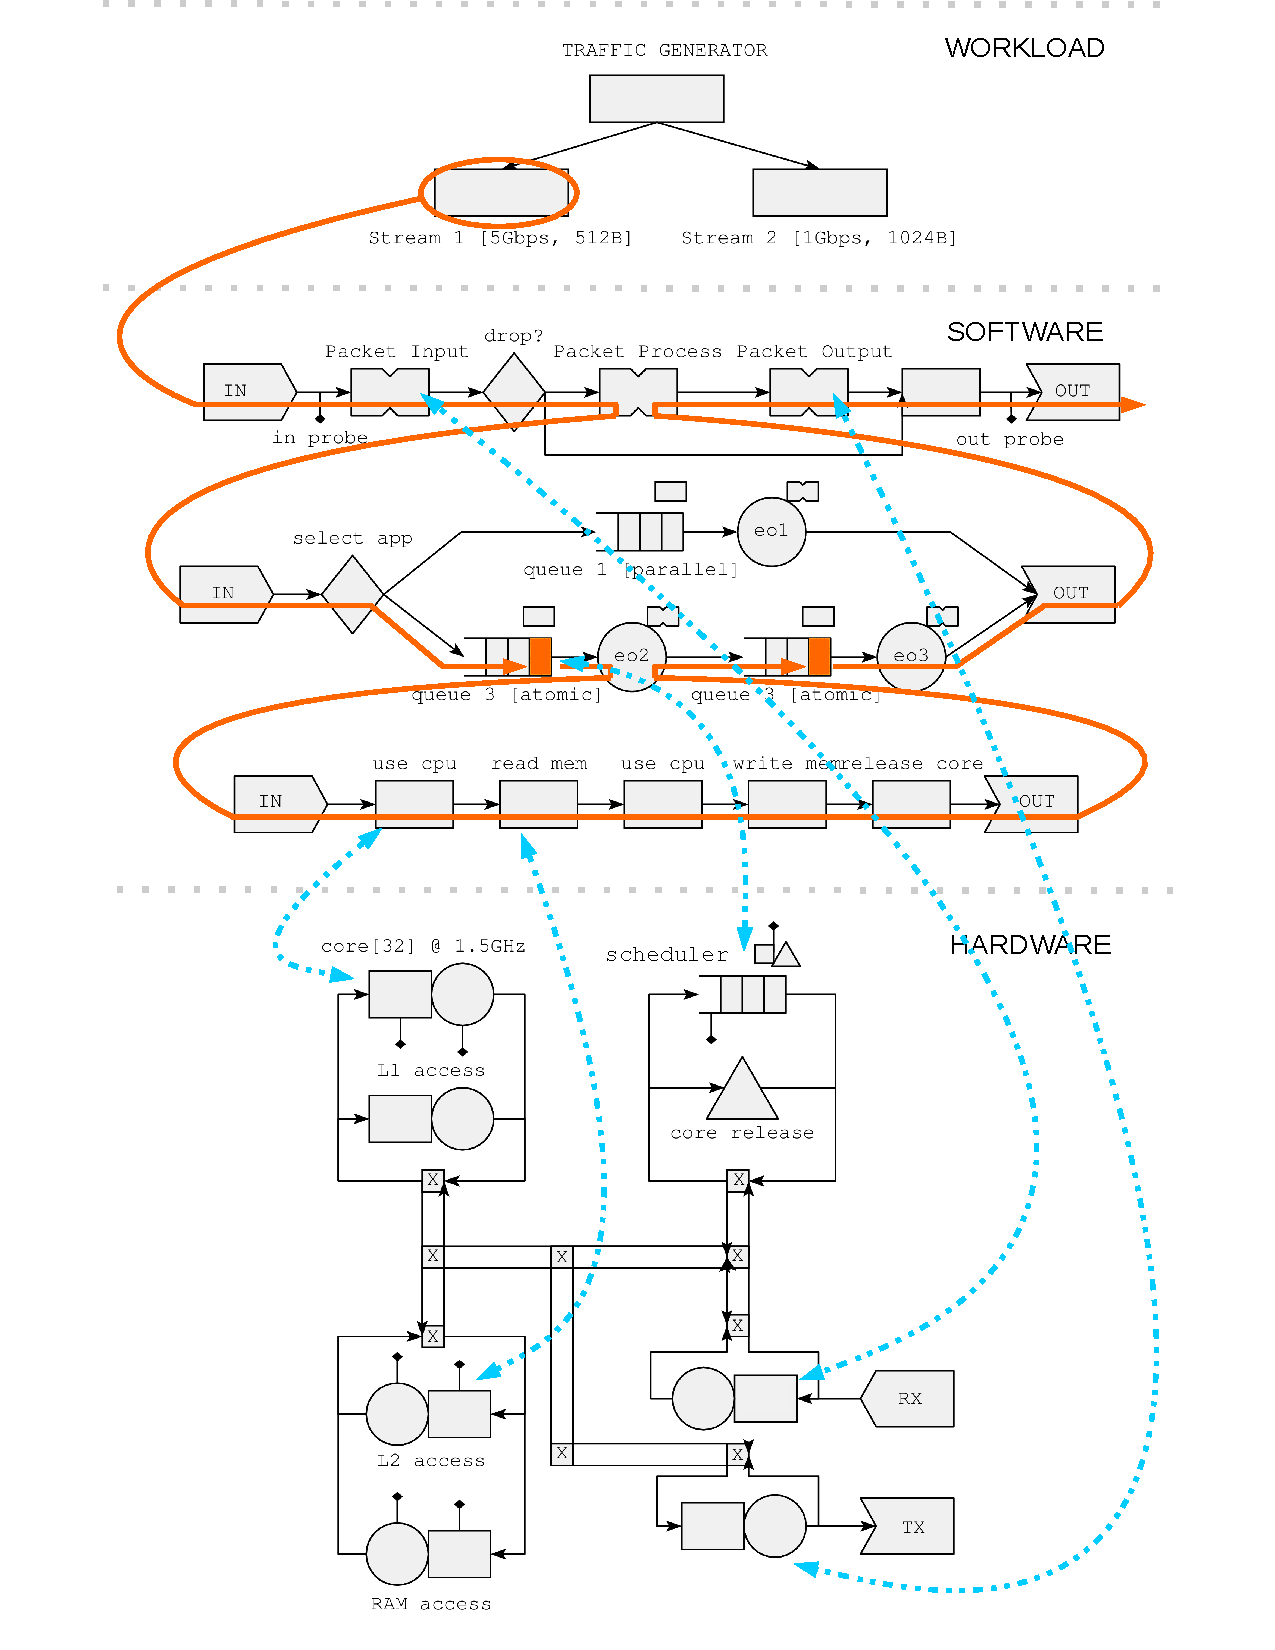
\includegraphics[width=\textwidth]{images/pse-models/fullmodel.pdf}
    \caption{Graphical presentation of the OCTEON II CN6880 PSE model. The workload model (top) generates network packets, which then flow through the software model (middle), consuming the hardware resources (bottom). The orange arrows represent an example of a packet's path through the software model, and the blue arrows the resource usage at each software model node.}
    \label{fig:full-model}
  \end{center}
\end{figure}

The workload model, at the top of the picture, consists of two packet streams. The \emph{TRAFFIC GENERATOR} node activates the two stream nodes, which again generate packets that enter the software layer. The workload nodes contain parameters, such as the application id's, that are used to control the packet flows in the software model.

% has a lifetime of 0.5 seconds, and it triggers the streams with interval drawn from a uniform distribution with parameters 0.00005 and 0.00015. The streams have lifetime of 0.0004 seconds, and interval drawn from a lognormal distribution. The packet sizes of the streams are defined with the size attribute. Both of the streams also specify an appId attribute that is used to define the processing application in the software model. The packets from both streams enter the IN node of the top level software model.

The software model is divided into several submodels. The top software level model consists of packet input, packet processing and packet output submodels. The submodel view of the packet input and packet output are omitted from the picture for the sake of simplicity, as in both of these phases, the core and memory usage is linearly dependent on the packet size with additional Gaussian noise. In the input phase, the packet consumes specific amount of core cycles for the header processing, and copies the packet header and the packet data to the memory. Packet output node copies the packet from the memory, and consumes certain amount of clock cycles for the packet checksum calculations.

The packet processing submodel is presented in the middle software layer. The select app node forwards each of the packets to one of the two packet processing application, based on the application id attribute defined in the workload model. The queue nodes represent the core scheduling done by the SSO hardware unit. The packets arriving in the upper application have priority of 1, and they can be processed in parallel. In the application below, there are 2 atomic queues with priority 3. When the packet receives the passive resource from SSO, it can enter the actual processing application, called execution object (eo). The execution objects are submodels that consume core cycles and memory similarly to the packet input and packet output submodels presented above. The SSO/core passive resource is released inside each execution object.

The hardware model is a simple one level model containing no submodels. In the bottom left hand corner, there are PKI and PKO devices providing processor cycles for the packet input and packet output phases. The only passive resource node, SSO, provides core access resources, which can be released with the core release node. The application cores are shown in the top left corner of the hardware layer. There are 32 cores, and a specific L1 cache access for each of them. The L2 and RAM memory resources provide the delay for reading and writing to memory.

The probes, attached to the SSO unit, the cores, and the memory nodes, are used to gather statistics from the execution. Each of the units has two probes, one to measure the resource usage, and the other to measures the queue for the corresponding resource. In this hardware model, the routing nodes (squares) and the edges connecting the resources do not have any functional meaning, but are used solely to mimic the graphical models of the CN6880 unit presented in~\cite{cavium:2010:fundamentals}.

\section{Modeling the Task Scheduler}
\label{sec:modeling-task-scheduler}
The Schedule/Synchronization/Order (SSO) unit has an important effect on the tasks' throughput times, as it controls the order in which the task get service from the application cores. This section first describes the application nodes used to model the SSO unit, and then the actual plug-in functions used to implement the scheduling functionality on the hardware model level.

% The SSO unit assigns the tasks to the processing cores.

% SSO unit needs to have a global

% The SSO unit schedules the tasks for the cores based on the

% Modeling a task processing application

% Figure~\ref{fig:full-model} has two different task processing applications.

% Before the task can be processed, it must wait for the SSO to schedule it on the core.

When modeling the applications on PSE, it is helpful to consider the flow from the task's perspective. When a task has passed the input processing, it is put into the SSO queue to wait to be scheduled on the application cores. Each time a core finishes its previous task, it requests for a new work from the SSO-unit, which then schedules a task based on the flow quality of service priority and work group.

\subsection{Application Models}
\label{application-models}

Each packet processing application consists of two parts: the SSO queue node, and the actual processing. The software layer in Figure~\ref{fig:full-model} presents an example of two main applications. The second application is divided into two sub-applications. The parameters for the first application's queue and execution object are shown in the Listings~\ref{lst:queue-attributes} and~\ref{lst:eo-attributes}, respectively.

\lstinputlisting[caption=The attributes of the SSO queue.,
                 label=lst:queue-attributes]{listings/queue-attributes.txt}

The first line in Listing~\ref{lst:queue-attributes} specifies the display title for the node, as shown in the Figure~\ref{fig:full-model}. The \emph{name} and \emph{type} attributes specify that the resource usage is passive, and the required resource provision entity is $core\_require$, i.e. the SSO. The parameters on lines 5-7 define the parameters that are used in the custom scheduling code on the hardware level. The \emph{$queue\_type$} value atomic specifies that two nodes entering the SSO from the same resource usage node, cannot be processed simultaneously. The \emph{$queue\_id$} is used to keep track of the tasks being processed, and \emph{$queue\_priority$} is used to globally prioritize tasks between the queues.

\lstinputlisting[caption=The attributes of execution object.,
                 label=lst:eo-attributes]{listings/eo-attributes.txt}

The execution object node parameters are shown in the Listing~\ref{lst:eo-attributes}. It is a simple submodel node. It specifies the display title, and the name of the submodel to be used. The \emph{file} attribute specifies the file that defines the submodel. Note that, each execution object submodel needs to release the SSO/core resource, as shown in the Figure~\ref{fig:full-model}.

\subsection{Scheduling/Synchronization/Ordering Unit}
\label{sec:SSO-unit}
To model the CN6880 processing cores' run-to-completion behavior, the SSO unit is modeled as a passive resource. Each time a task is entering a processing application, it first acquires the passive SSO resource. The amount of available passive SSO resources is equal to the processing cores in the system, and a task cannot use processing core without holding the SSO resource.

% The SSO scheduling is done in the SSO node presented in the hardware level in Figure~\ref{fig:full-model}. The actual scheduler function is written as a plug-in code, using the interface provided by PSE. The custom scheduling in PSE requires two functions, which are written in C-code: the selection function, and the reserve function. Each time a task enters a resource usage node in the task graph, the reserve function is called. The reserve function either

To model the SSO unit, custom scheduling functions are required. These are modeled using PSE's custom plug-in interface, presented in chapter~\ref{chapter:mechanism-for-extended-queue-disciplines}. The functionality is implemented in two custom functions, written in C-code: the selection function, and the reserve function. The resource node parameters are changed to use these functions. The parameters of the SSO node used in the example model are presented in the Listing~\ref{lst:RNS-attributes}.

\lstinputlisting[caption=The attributes of the SSO node to determine the custom scheduler.,
                 label=lst:RNS-attributes]{listings/SSO-attributes.txt}

The first three lines specify the node title, name, and capacity. The capacity is set to the amount of available processing cores, meaning that no more than 32 tasks can be processed simultaneously. The \emph{discipline} parameter \mbox{CUSTOM}, on line 5, specifies that a custom scheduler is used instead of the built-in scheduling functions. The \emph{file} parameter specifies the path of the C header file that declares the scheduling functions. The \emph{$select\_function$} and the \emph{$reserve\_function$} parameters specify the two functions that are required to implement the scheduling logic.

The reserve function is called each time a task enters a resource usage node in the resource usage model, and it determines whether the task can immediately be served, or if it has to wait for the service. If the task can be processed immediately, it is inserted to the processing queue of the resource, and to the waiting queue otherwise. If the task gets put to the waiting queue, the reserve function also needs to reorder the queue.

Listing~\ref{lst:CUSTOM_reserve} describes the reserve function used to model the SSO. The function takes four input arguments: \emph{r} contains the data of the resource being reserved; \emph{queue} is a pointer whose value is assigned either to the processing queue or the waiting queue; \emph{position} is a pointer, whose value is assigned to the position in the queue; \emph{$new\_client$} holds the parameters, defined in the workload and resource usage models, of the new task.

\lstinputlisting[caption=The $CUSTOM\_reserve$ function for SSO.,
                 label=lst:CUSTOM_reserve]{listings/CUSTOM_reserve.c}

On the lines 11-39, the reserve function attempts to place the task in the processing queue. The if-statement, on line 11, checks if the resource capacity is full. If there are available cores, then the processing conditions are checked, by going through all the cores, as shown in the for-loop on lines 21-32. If the new task's flow is marked atomic (in the reserve node in resource usage graph), and another task from the same flow is being processed on one of the cores (if-condition on lines 25-26), then the for-loop breaks, and the task gets set to the waiting queue. If a core is not processing, and the flow's coremask permits processing on the core (if-condition on line 31), we assign core's index to variable \emph{j}. Finally, if there is available core (\emph{j} is smaller or equal than the resource capacity) and none of the tasks from the same atomic flow are being processed, we set the queue to point to the resource's processing queue, and the position to the variable \emph{j}, and return.

If the processing conditions are not met, i.e. the execution goes past the if-block, then the task is set into the waiting queue. Line 43 assigns the \emph{queue} to point to the waiting queue of the resource. The for-loop on lines 46-48 finds the first task with larger priority, at index \emph{i}, and the for-loop on lines 51-53 moves all the higher priority tasks one step further on the queue. Finally the index \emph{i} is assigned to \emph{position}, and the function returns.

Each time a core ends a processing of a task, a new task is selected for the processing, using the custom select function. Listing~\ref{lst:CUSTOM_select} shows the code used for the select function to model the SSO.

\lstinputlisting[caption=The $CUSTOM\_select$ function for SSO.,
                 label=lst:CUSTOM_select]{listings/CUSTOM_select.c}

$CUSTOM\_select$ takes the resource \emph{r}, and the index of the released core \emph{$release\_index$} as an input. The outer for-loop, starting at line 7, goes through all the tasks in the waiting queue, and finds the first task that satisfies the processing constraints, similarly as the reserve function. Line 10 checks if the waiting task's coremask allows the task to be processed on the core. If the waiting task's flow is atomic (line 12), we need to go through all the processing cores to check that there is no task being processed from the same flow (lines 18-24). If the task was not atomic, or no tasks from the same flow were being processed, the function returns the index of the task in the waiting queue. Otherwise we move to the next waiting task and repeat. If no task from the waiting queue can be scheduled, the function returns $RNS\_LARGE$. The RNS automatically moves the clients when it removes the task from the waiting queue.

%%% Local Variables:
%%% mode: latex
%%% TeX-master: "thesis-hartikainen"
%%% End:

\chapter{Demonstrative Experiments}
\label{chapter:demonstrative-experiments}

This chapter presents two demonstrative simulation experiments done on the NPU model presented in Chapter~\ref{chapter:modeling-a-packet-processing-system}. The goal of the experiments is to demonstrate how the parallel mechanisms of a task based-programming model, i.e. queue types, priorities, and coremasking, affect the scheduler, and hence the packet throughput and latency. At the same time, it validates our NPU model and the PSE's implemented plugin-code functionality.

In the first experiment, we will use the global queue information to control the resource provision based on global queue priorities and disciplines defined in the software queues. The second experiment presents the use of queue coremasks, to control the use of specific hardware resources, through the software model.

\section{Experiment Setup}
\label{sec:experiment-setup}

Both experiments are run on the hardware model represented in Figure~\ref{fig:experiment-hardware}. The model consists of six active resources. The PKI and PKO units are consumed by the input and output phases of the packet flow, respectively. Each 32 processing cores have a L1 cache associated with it, and the L2 cache and RAM are shared between the cores. The cores are served as first come first serve basis, as the scheduling logic is taken care of by the SSO unit.

\begin{figure}[]
  \begin{center}
    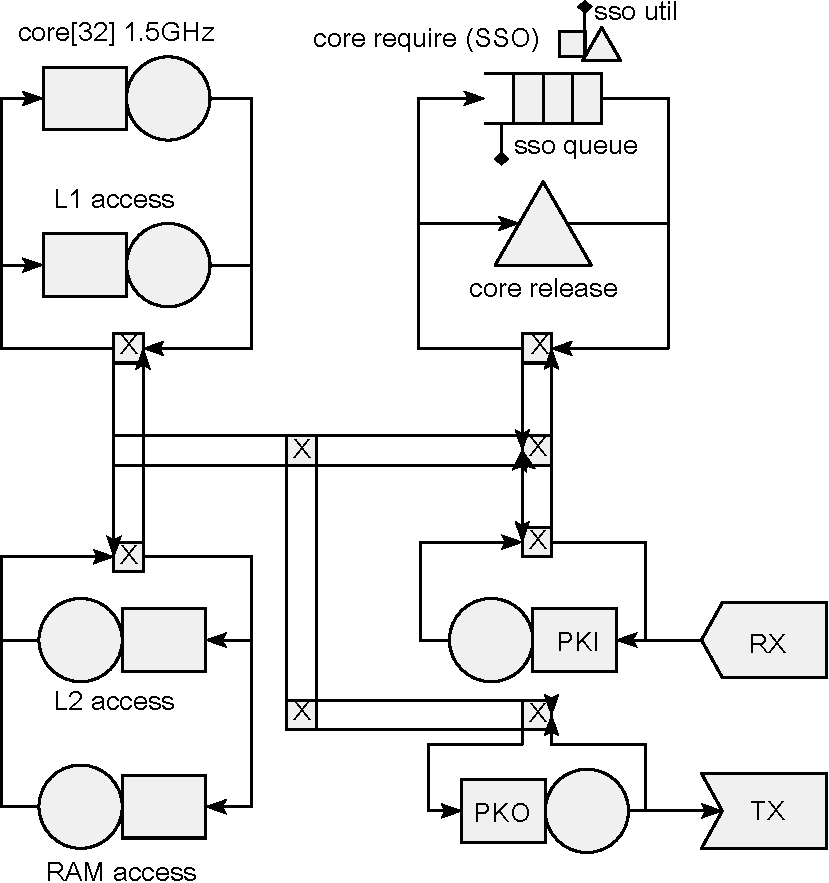
\includegraphics[width=0.6\textwidth]{images/pse-models/experiment-hardware.pdf}
    \caption{Resource provision model (hardware) used in the experiments. The model represents the Cavium Octeon CN6880 network processing unit.}
    \label{fig:experiment-hardware}
  \end{center}
\end{figure}

The SSO unit uses the custom scheduling functions presented in the section~\ref{sec:SSO-unit}, enabling the use of atomicity, queue priorities, and coremasks. The core release is a typical release node referring to the SSO unit.

The same high level software model is used for the both experiments, as seen in the Figures~\ref{fig:exp1-software} and~\ref{fig:exp2-software}. The \emph{Packet Input} and \emph{Packet Output} nodes consume the PKI and PKO units as discussed in the section~\ref{sec:characteristic-measurements}, delaying the packets relative to their size, according to the equation~\ref{eq:1}. The workload and packet process submodels are unique for both experiments.

We gather two different metrics of the system. First, we are interested in the core utilization and queue lengths for each processing step. These are measured by the probes attached to the SSO unit as shown in hardware model in Figure~\ref{fig:experiment-hardware}. Secondly, we are interested in the packet latencies. They are measured by calculating the time difference between the \emph{out probe} and the \emph{in probe} (Figures~\ref{fig:exp1-software} and~\ref{fig:exp2-software}) for each packet. All the probes write absolute traces of the packets.

\section{Experiment 1: Global Queue Interrelations}
The first experiment consists of two different simulations and measurements. We will first demonstrate a packet processing application, whose throughput is limited due to the bottleneck occurring from a slow atomic processing. The application is then modified, extracting part of the atomic execution object into parallel, thus breaking the bottleneck.

The workload model consists of a single packet stream, which is generated from a two level workload model, presented at the top in Figure~\ref{fig:exp1-software}. The \emph{TRAFFIC GENERATOR} node triggers its child node with interval $RNS\_random\_uniform(5*10^{-5}, 15*10^{-5})$ seconds, and lifetime of 0.05 seconds. The child node creates 512B packets with interval $5.1~*~10^{-8}~* RNS\_random\_lognormal(-10, 0.9)$ seconds for $4*10^{-5}$ seconds.

The two different applications used in the experiment are shown in the software model after the \emph{select app}-node. The lower and upper application are referred as \emph{application 1} and \emph{application 2}, respectively. The application selection is done in the workload model by the \emph{AppId} attribute.

Application 1 consists of two processing steps, both consuming CPU and memory for the range of 5000 clock cycles. The first step consists of parallel, priority 2 queue (A), and the second one is done atomically with priority 1 queue (B). Application 2 is a modified version of the first packet processing application, where the second processing step is split into parallel and atomic steps. The release nodes are omitted from the software model for clarity.

\begin{figure}[]
  \begin{center}
    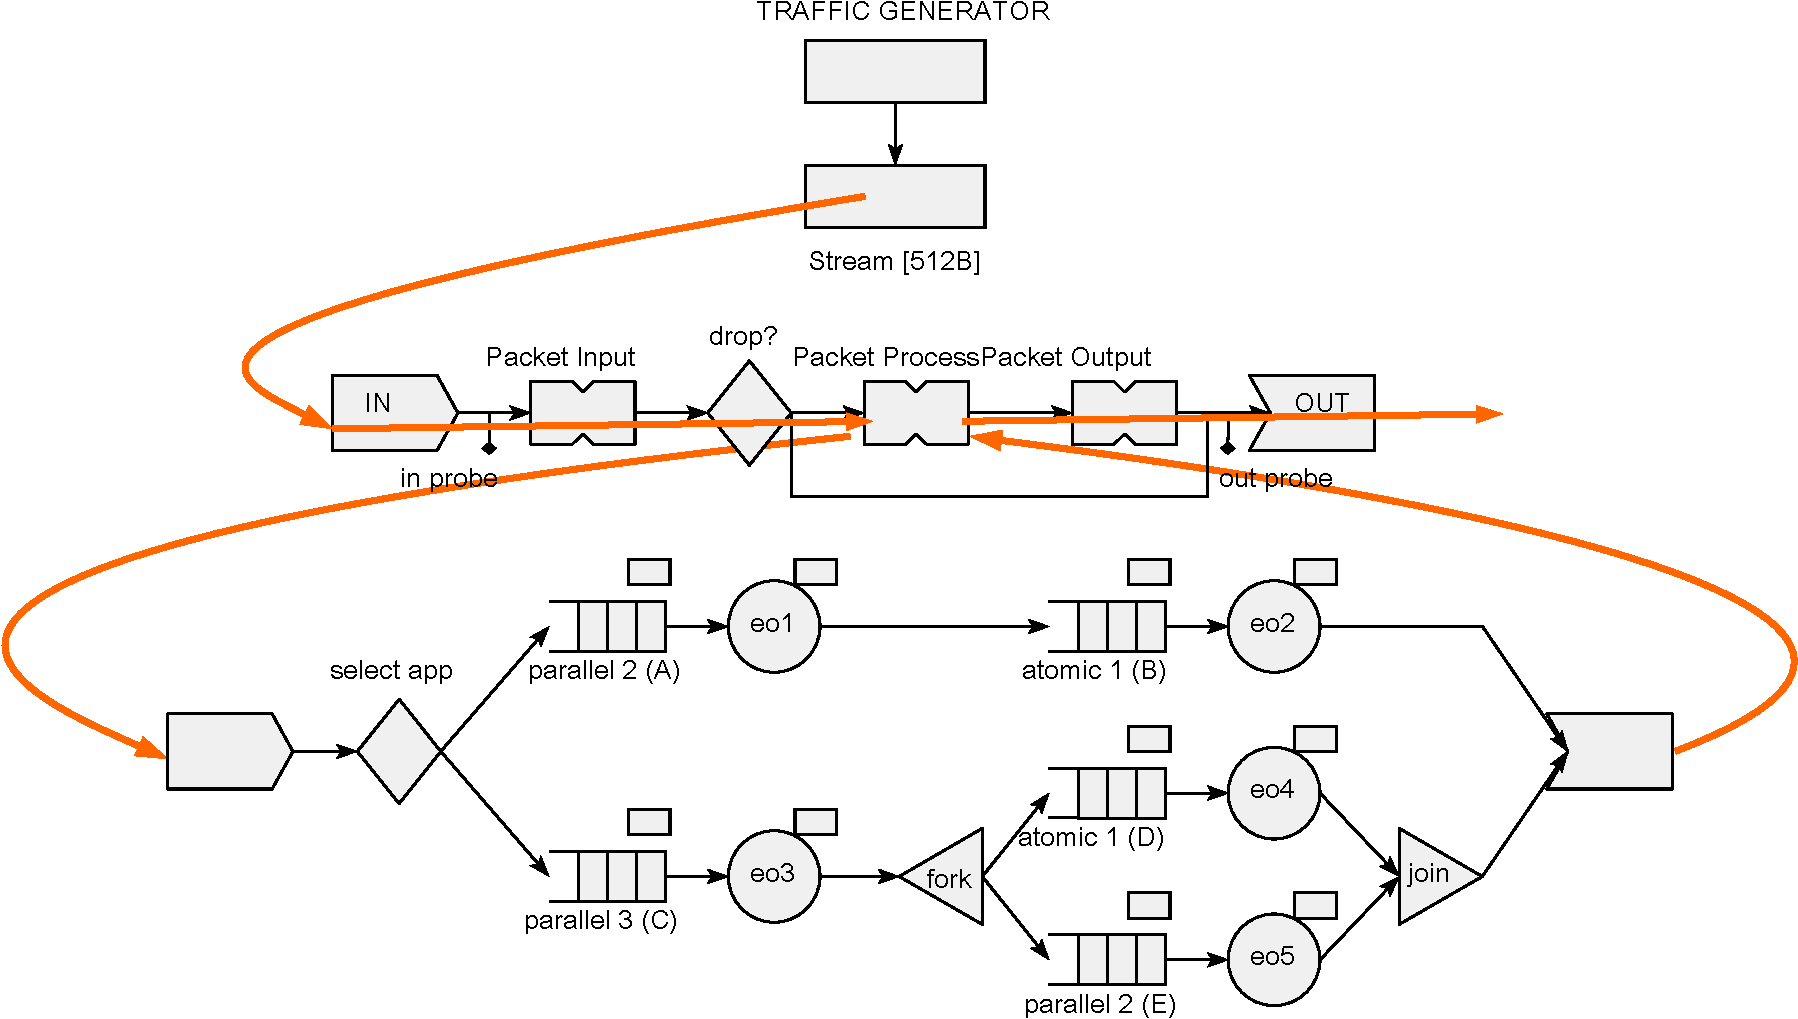
\includegraphics[width=\textwidth]{images/pse-models/exp1-software.pdf}
    \caption{Workload and resource usage (software) models used in the first experiment. The atomic queue in the upper application (application 1) produces a bottleneck to the system. The application 2 below removes this bottleneck by extracting part of the processing into parallel.}
    \label{fig:exp1-software}
  \end{center}
\end{figure}

\subsection{Simulation Measurements}
\label{sec:exp1-simulation-measurements}
The system was simulated using both applications separately, and the data from the probes were post-processed. We grouped the number of tasks in the SSO/core queue, by the processing step.

Figures~\ref{fig:app1-queue2} and~\ref{fig:app1-latency} present the data from the first simulation using the packet processing application 1. Figure~\ref{fig:app1-queue2} describes the number of tasks in the SSO/core queue, that are from the atomic resource usage queue, with respect to simulation time. The corresponding graph for the first queue is omitted, as none of that tasks from it end up in the waiting queue. Figure~\ref{fig:app1-latency} presents the latency of each packet through the whole system.

\begin{figure}[]
  \begin{center}
    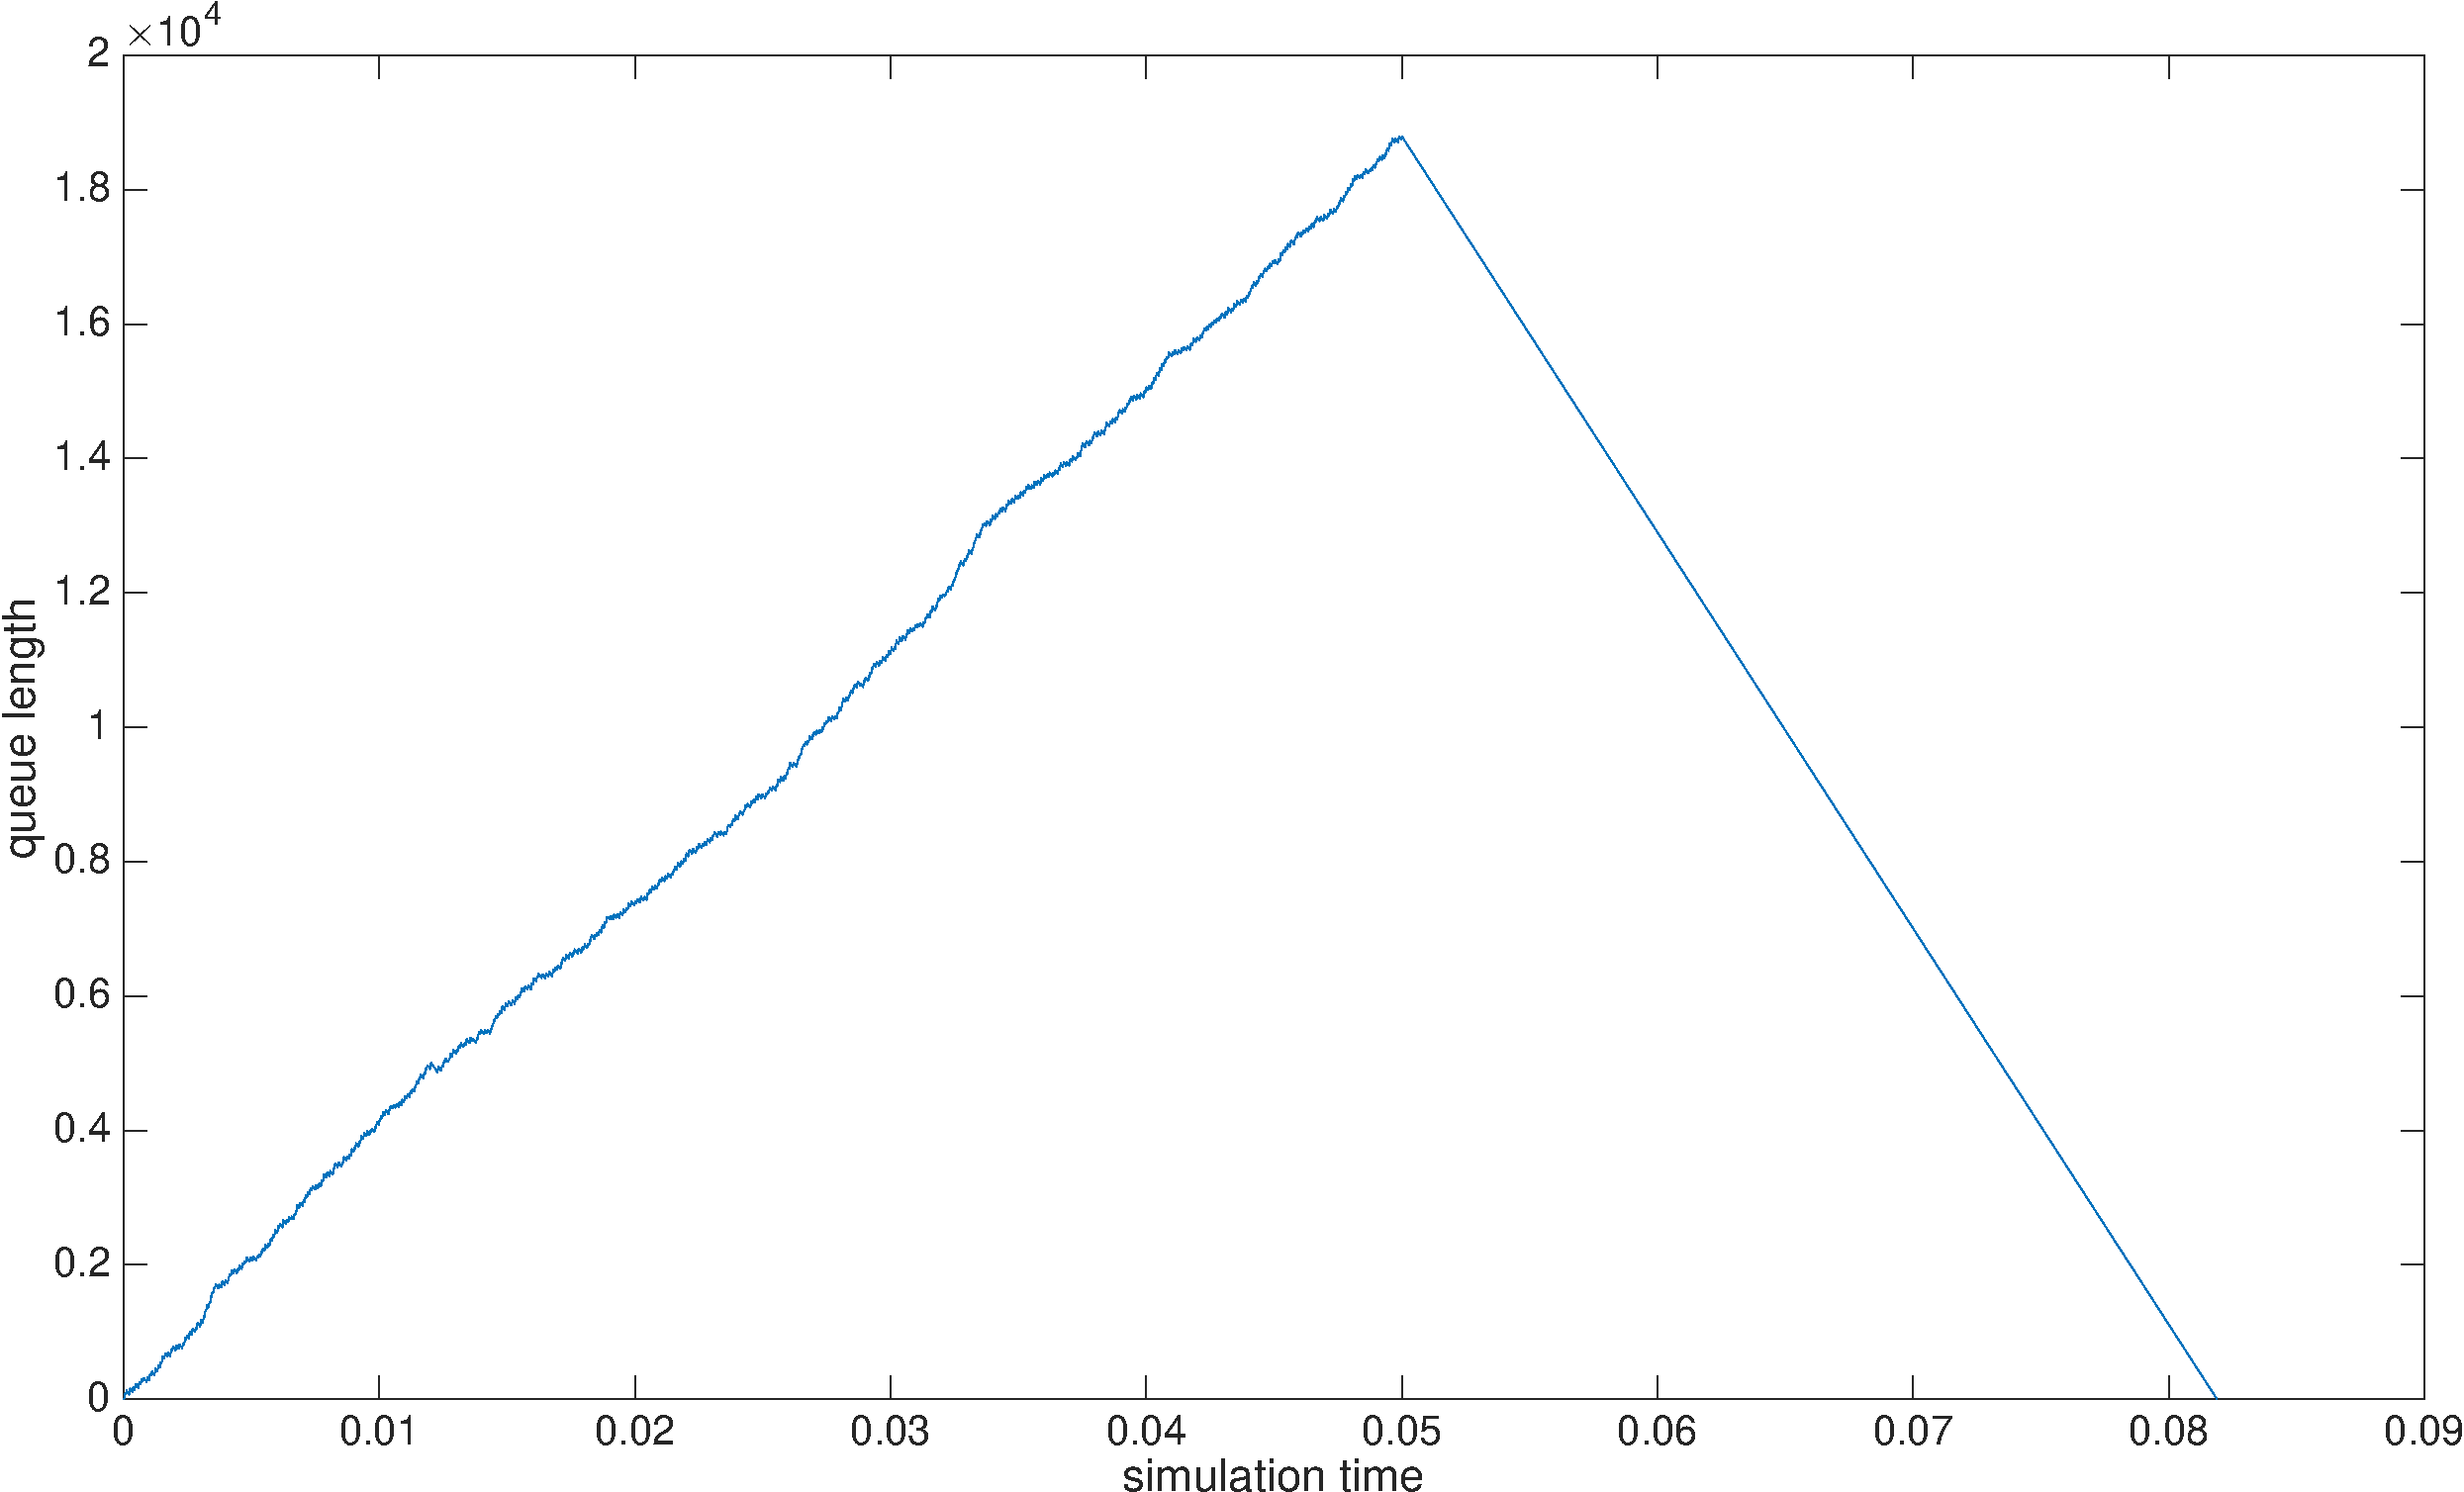
\includegraphics[width=\textwidth]{images/experiment/app1-queue2.pdf}
    \caption{Application 1: The number of tasks in the SSO/core queue, with respect to simulation time, from the second resource usage queue.}
    \label{fig:app1-queue2}
  \end{center}
\end{figure}

\begin{figure}[]
  \begin{center}
    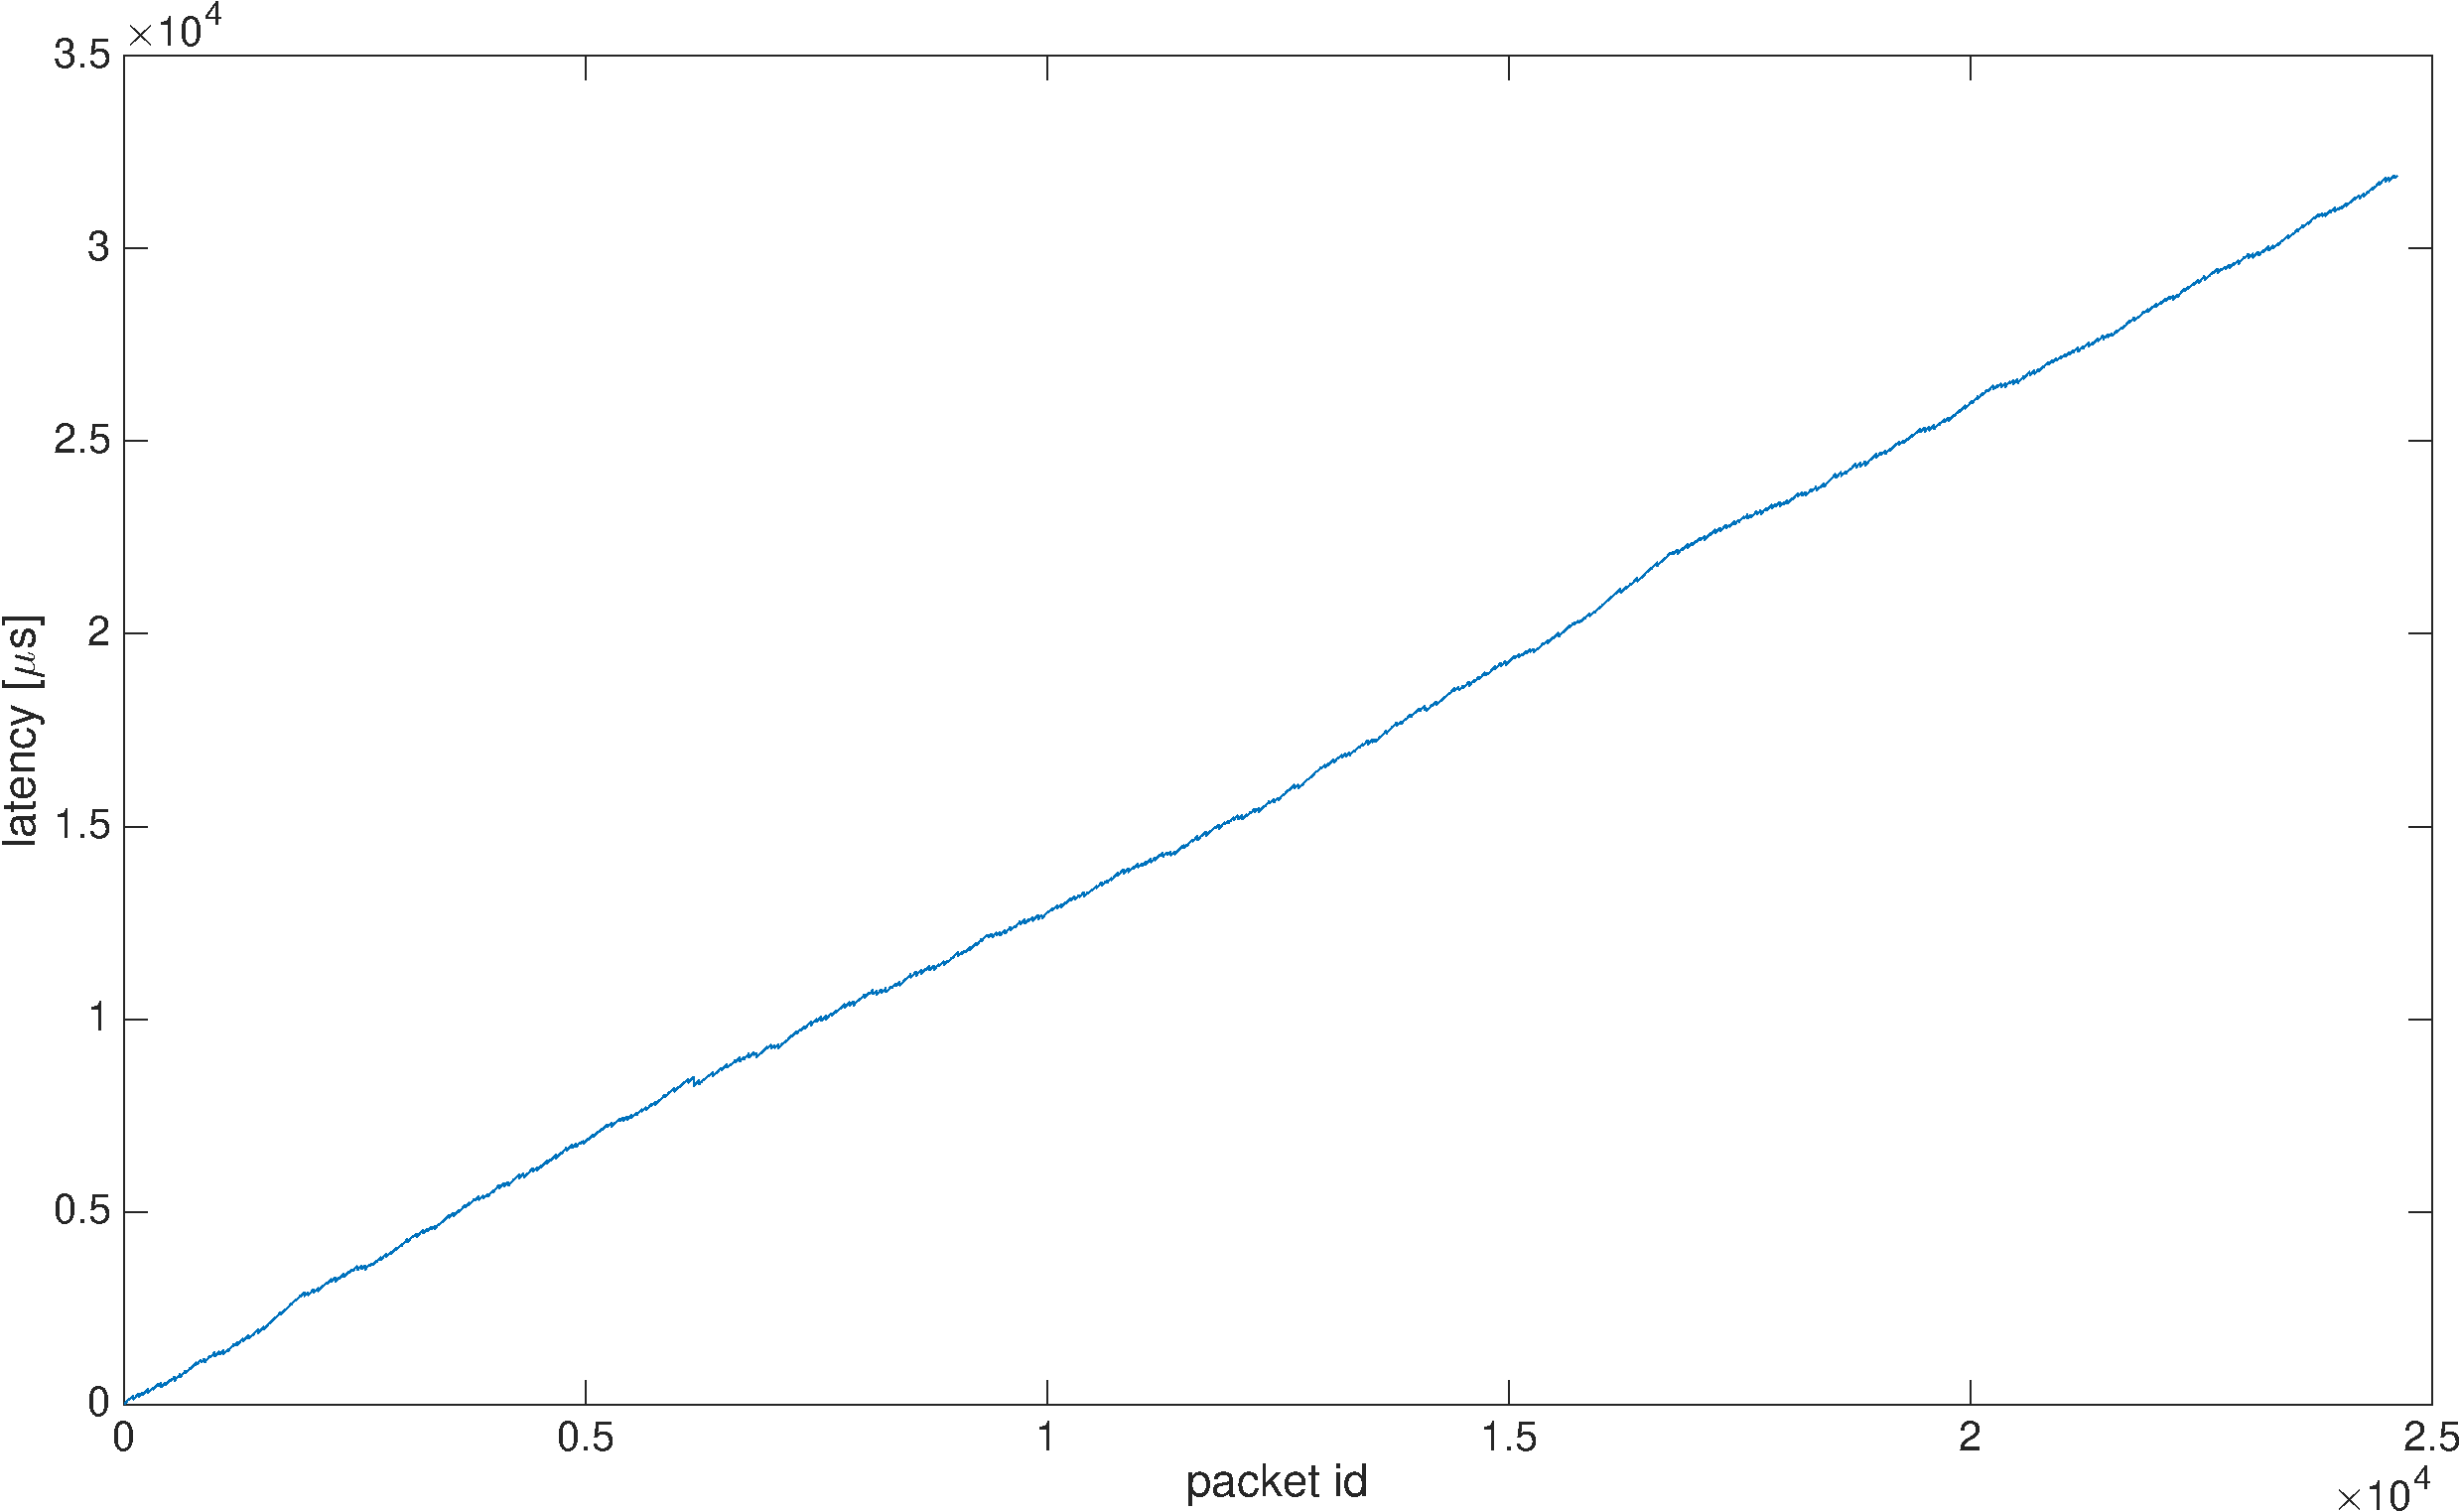
\includegraphics[width=\textwidth]{images/experiment/app1-latency.pdf}
    \caption{Application 1: Latency of the packets through the system.}
    \label{fig:app1-latency}
  \end{center}
\end{figure}

As shown in the Figures, the processing in the second execution object of application 1 is so heavy that the tasks accumulate into the waiting queue, and thus the packet latency keeps growing until the workload ceases.

The second application modifies the system by parallelizing part of the atomic processing. Figures~\ref{fig:app2-queue2} and~\ref{fig:app2-latency} present the data from the second application simulation. Figure~\ref{fig:app2-queue2} shows the number of tasks in the SSO/core queue, that are from the atomic resource usage queue, with respect to simulation time. Figure~\ref{fig:app2-latency} presents the latency of the packets through the whole system. Neither of the parallel queues have tasks in the waiting queue of the SSO/core during the simulation.

\begin{figure}[]
  \begin{center}
    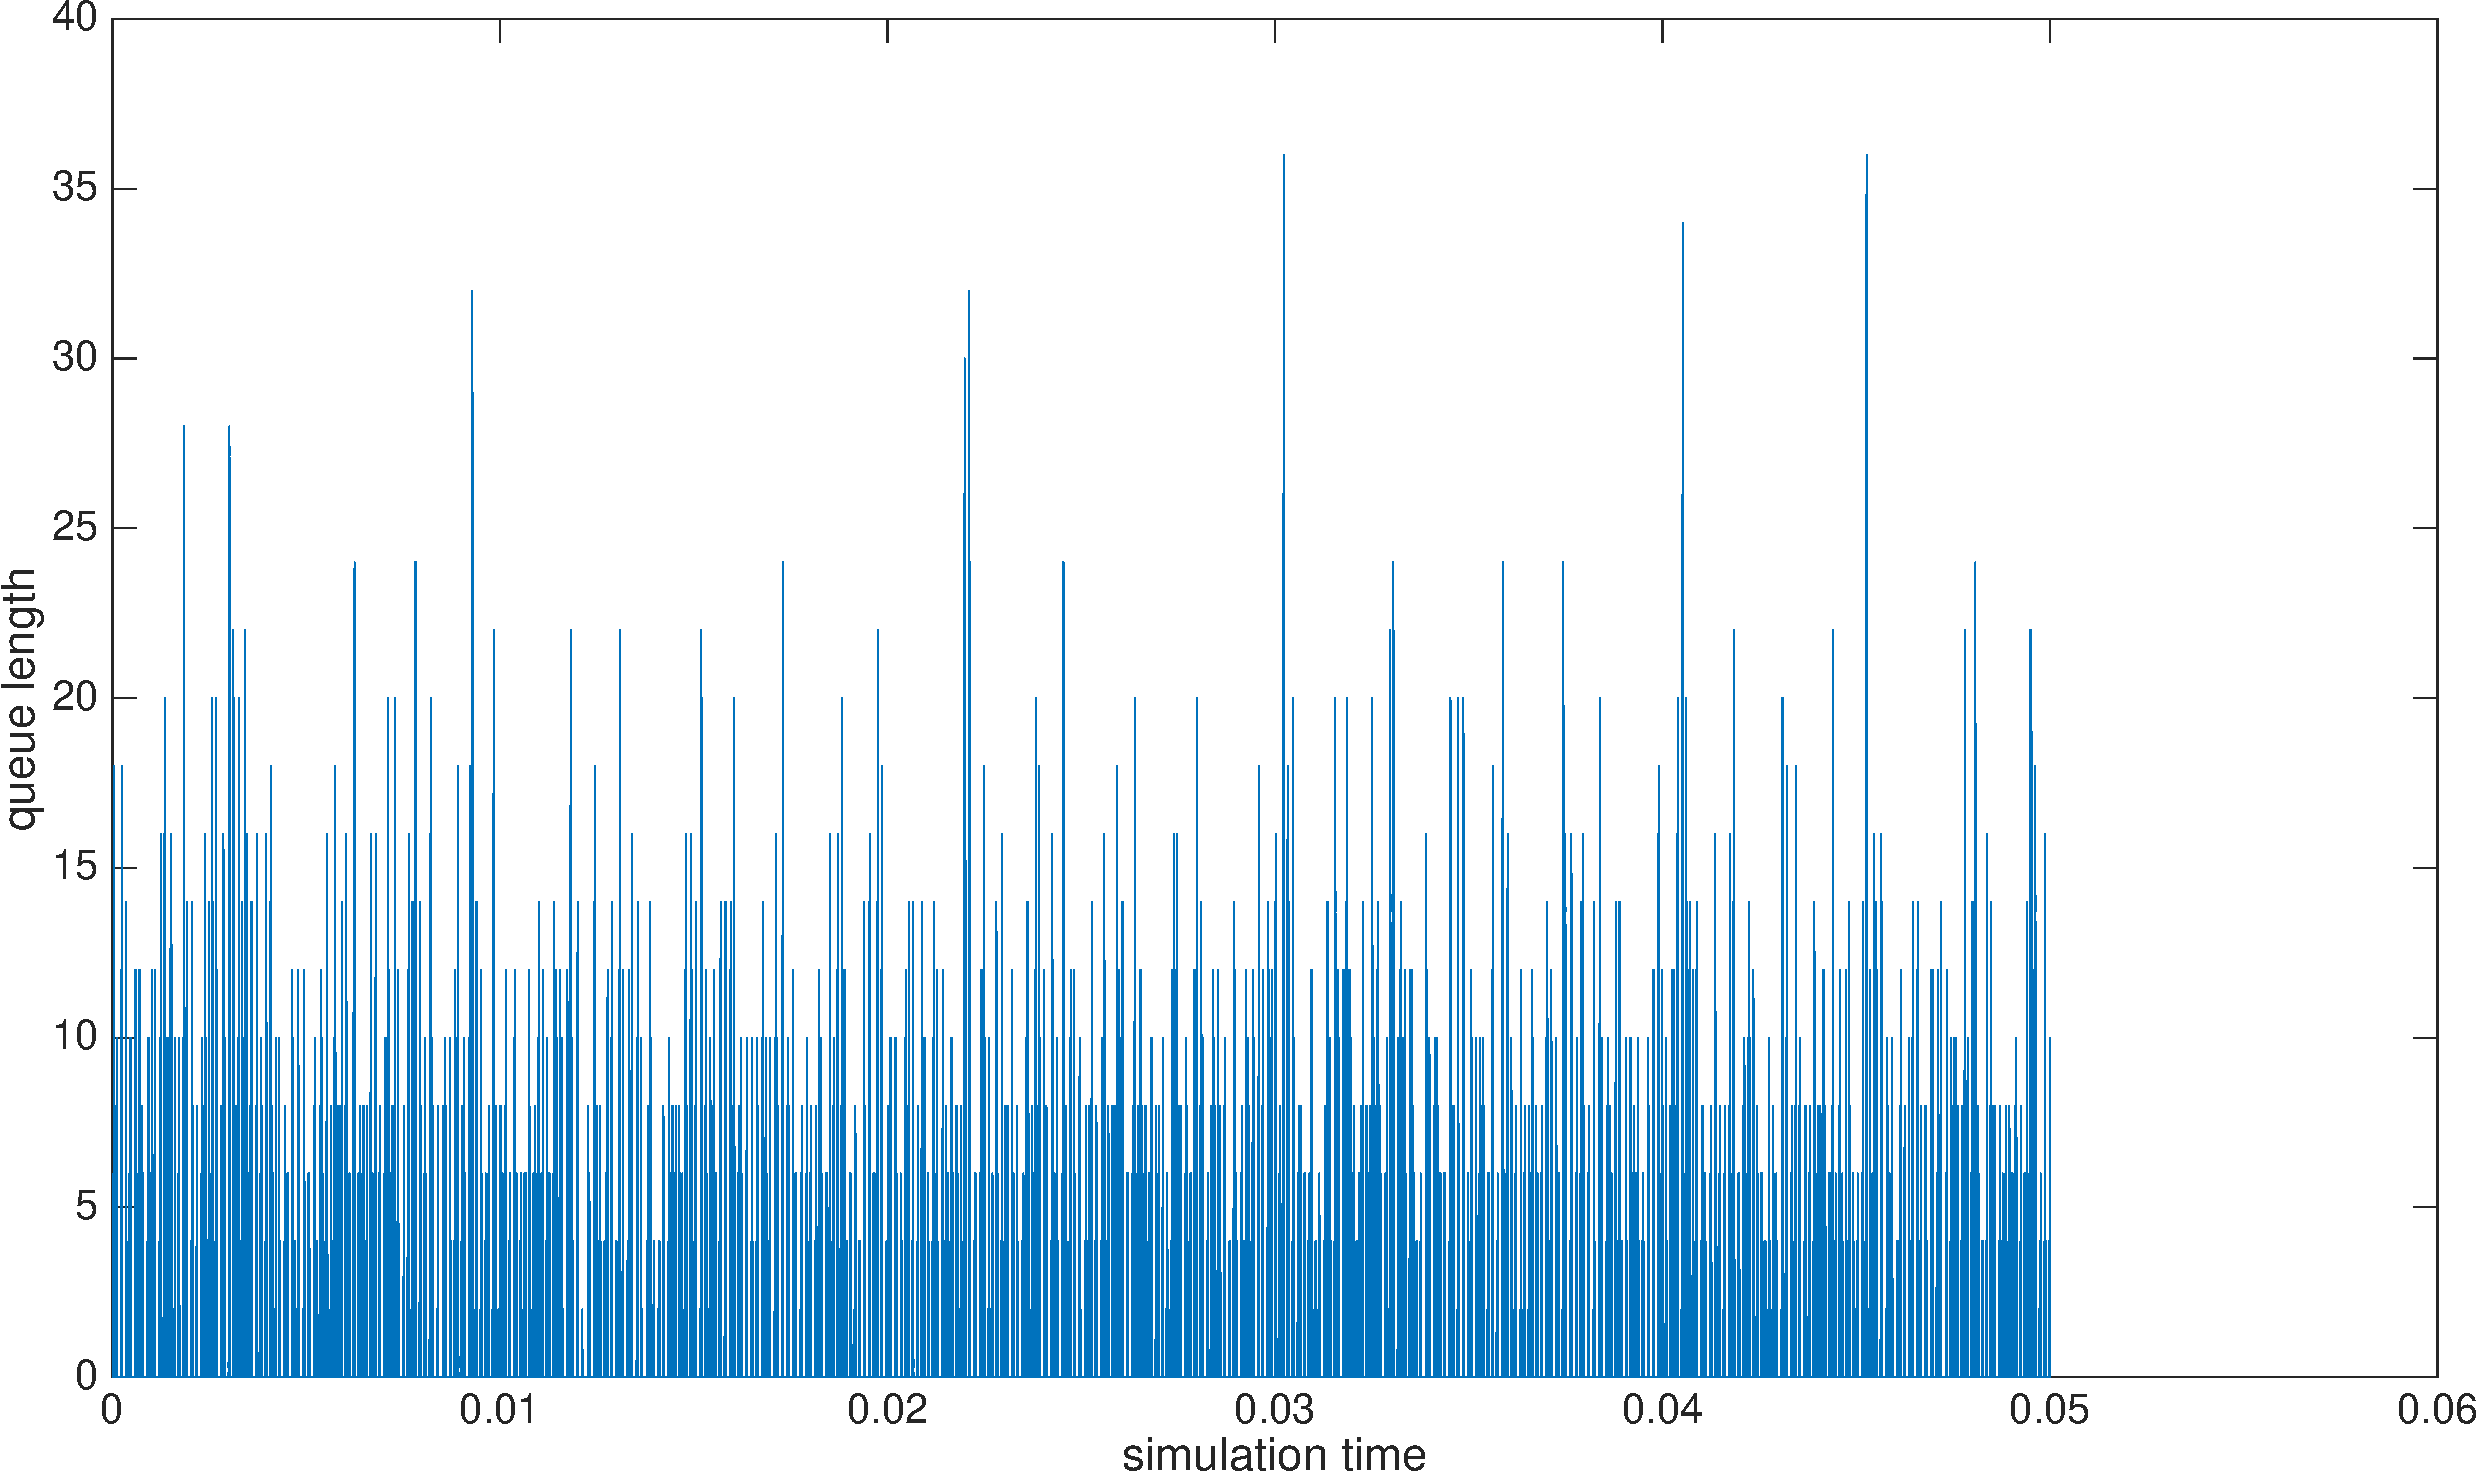
\includegraphics[width=\textwidth]{images/experiment/app2-queue2.pdf}
    \caption{Application 2: The number of tasks in the SSO/core queue, from the second resource usage queue.}
    \label{fig:app2-queue2}
  \end{center}
\end{figure}

\begin{figure}[]
  \begin{center}
    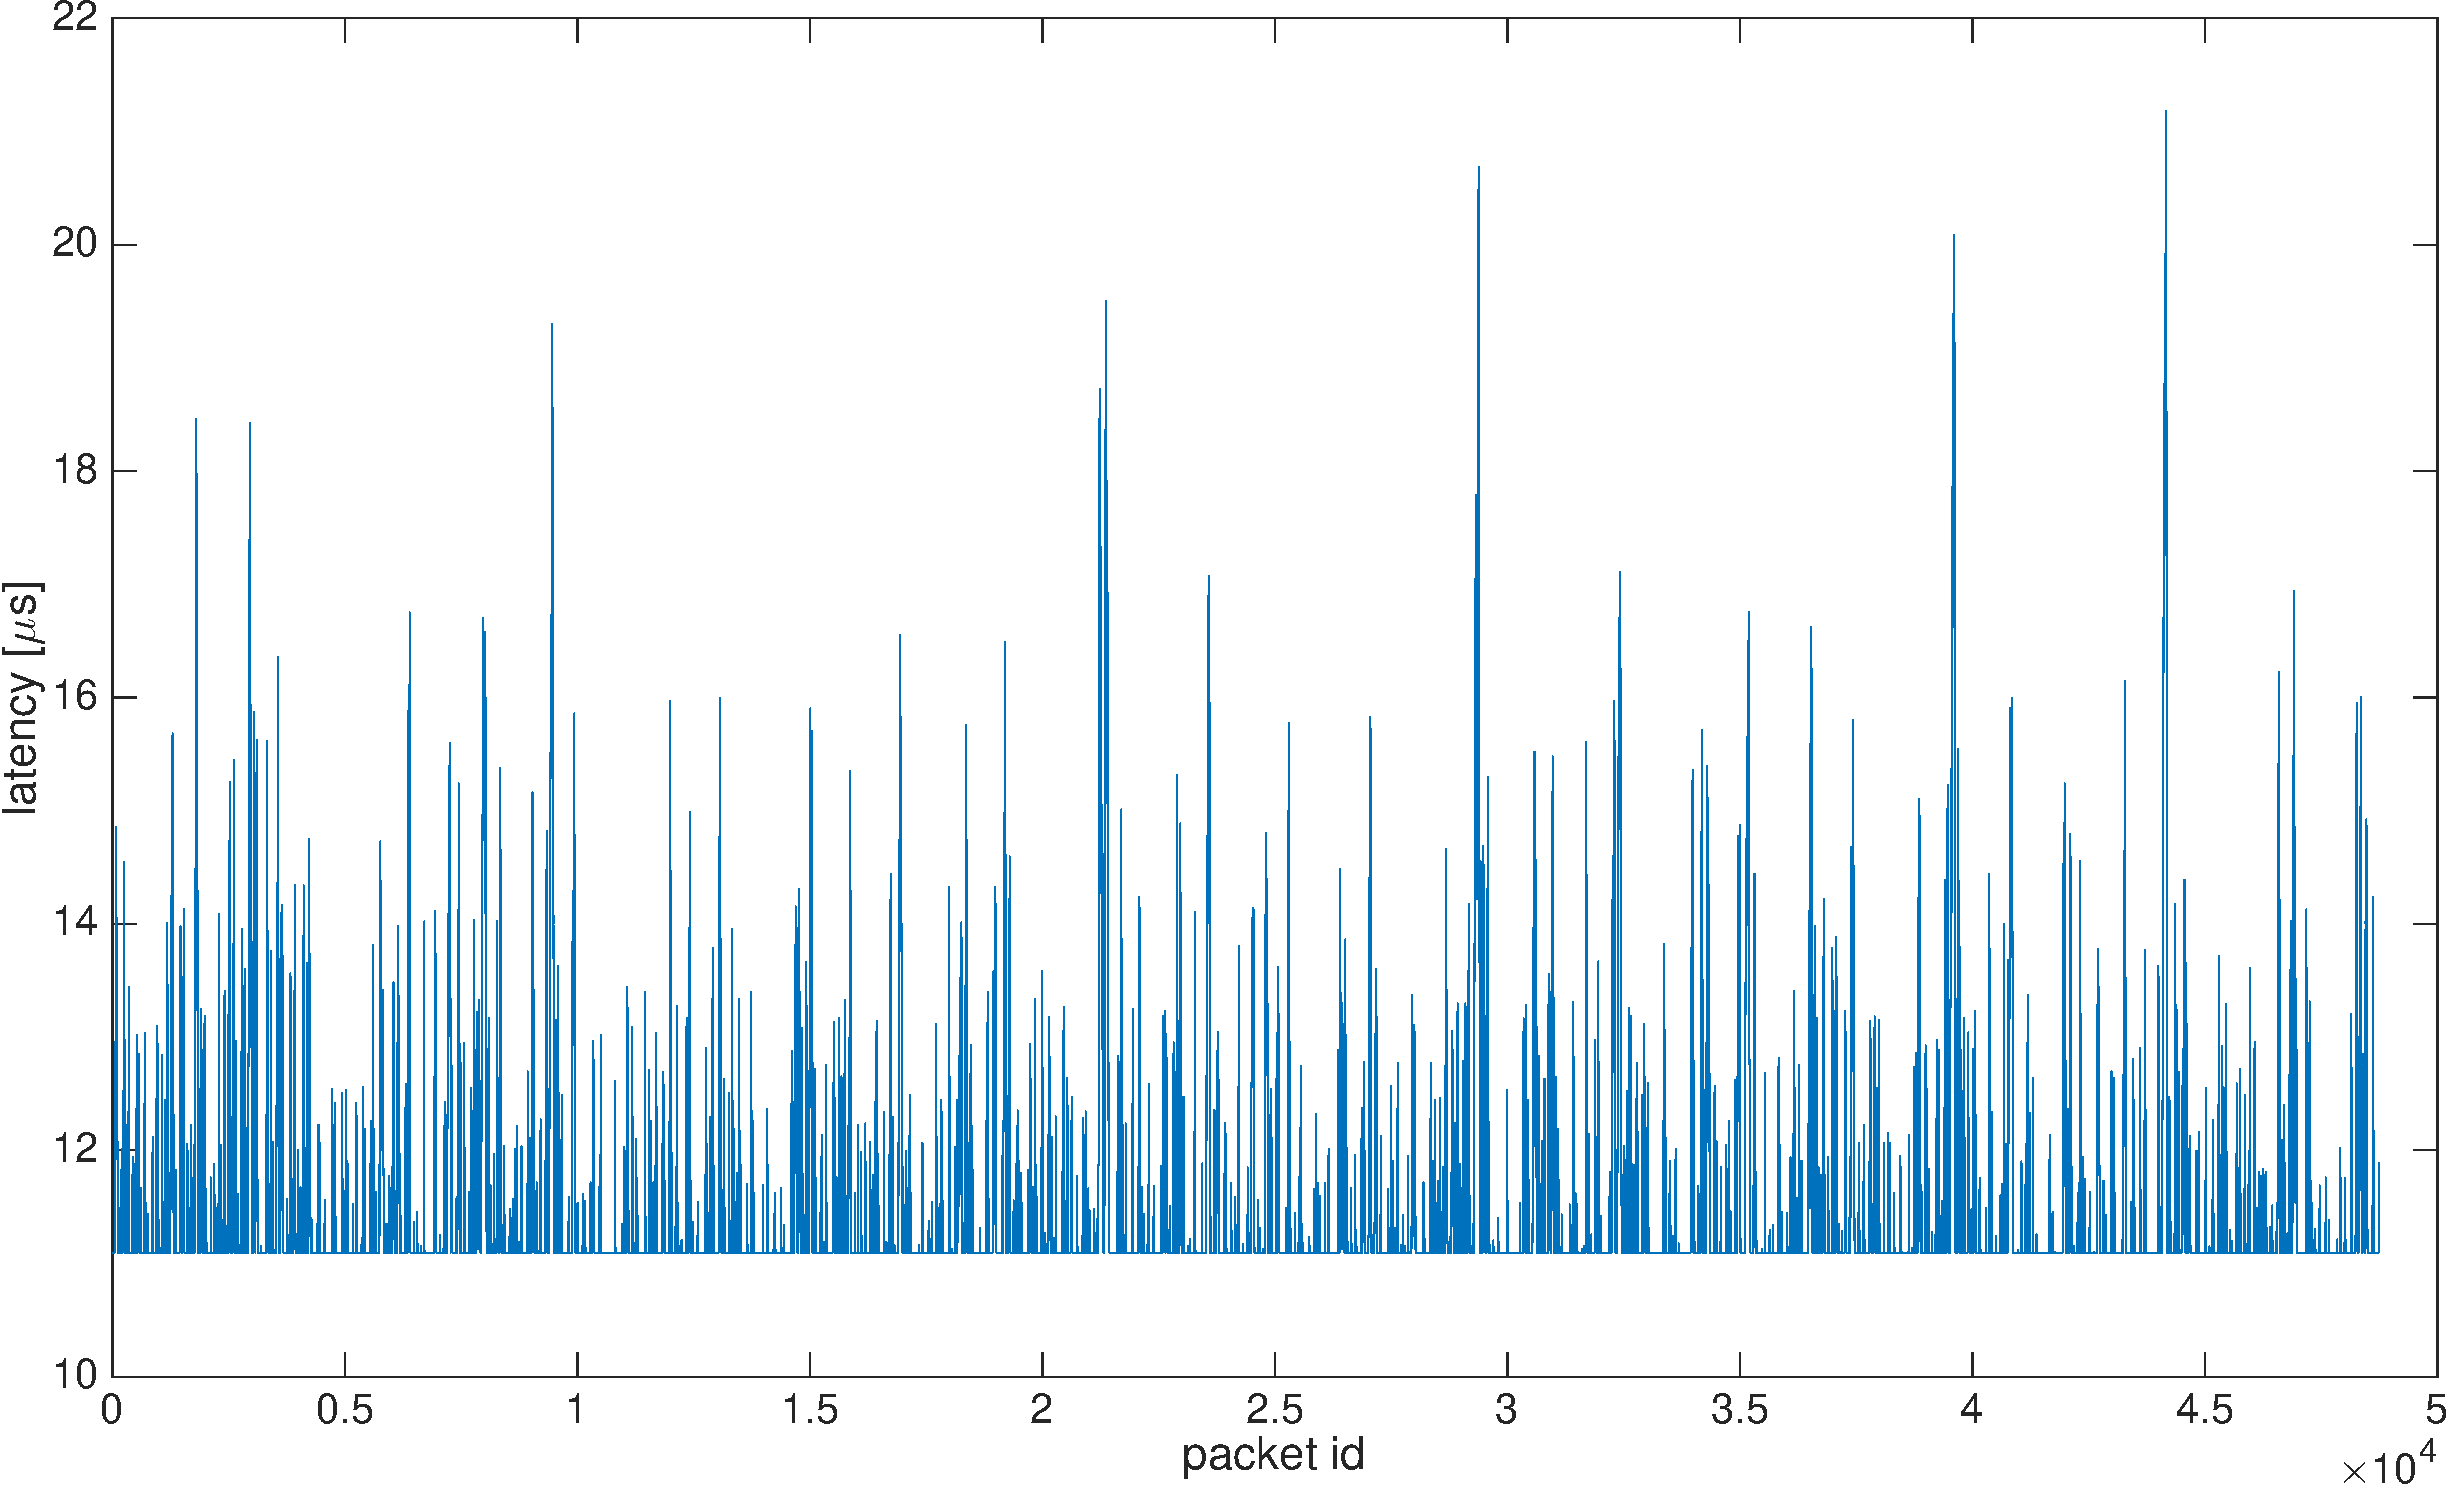
\includegraphics[width=\textwidth]{images/experiment/app2-latency.pdf}
    \caption{Application 2: Latency of the packets through the system.}
    \label{fig:app2-latency}
  \end{center}
\end{figure}

As the shown in the Figures~\ref{fig:app2-queue2} and~\ref{fig:app2-latency}, the latencies of the second application stay within 22$\mu$s, reducing the queue length below 40 over the whole simulation period.

\section{Experiment 2: Queue Coremasks}
% app1 heavy
% app2 light

The second experiment demonstrates the packet flow control via queue coremasks. The experiment consists of two packet flows and dedicated application processing them, as presented in Figure~\ref{fig:exp2-software}. The first packet stream (presented as orange), presents a higher OSI-level application data, such as video stream, which is processed on a heavy execution object. The second stream (presented as blue), on the other hand, consists of packets whose processing is done on fast processing application with strict latency requirements.

The \emph{TRAFFIC GENERATOR} node triggers its child nodes with interval $RNS\_random\_uniform(5*10^{-5}, 15*10^{-5})$ seconds, and lifetime of 0.05 seconds. \emph{Stream 1} and \emph{Stream 2} create 512B packets with interval $6.1*10^{-7}~*~RNS\_lognormal(-10, 0.9)$ and $10^{-6}~*~RNS\_lognormal(5, 10)$ seconds for $4*10^{-5}$ and $10^{-5}$ seconds, respectively. The heavy application consumes the CPU and memory for a total of about 50000 cycles per 512B packet, while the light application packets are processed for tenth of that, in 4500 cycles.

We will again perform two different simulations and measurements. The first one is carried out by allowing the heavy application to be processed on all the 32 processing cores. Despite the light flow being processed on higher priority queue, the processing of the heavy flow has an effect to the worst-case latency of the light flow packets. This happens due to the run-to-completion model of the cores, where light flow packets may have to queue for a core while the heavy tasks finish. In the second simulation, the heavy application processing is limited to 30 cores, dedicating two cores for the light application.

\begin{figure}[]
  \begin{center}
    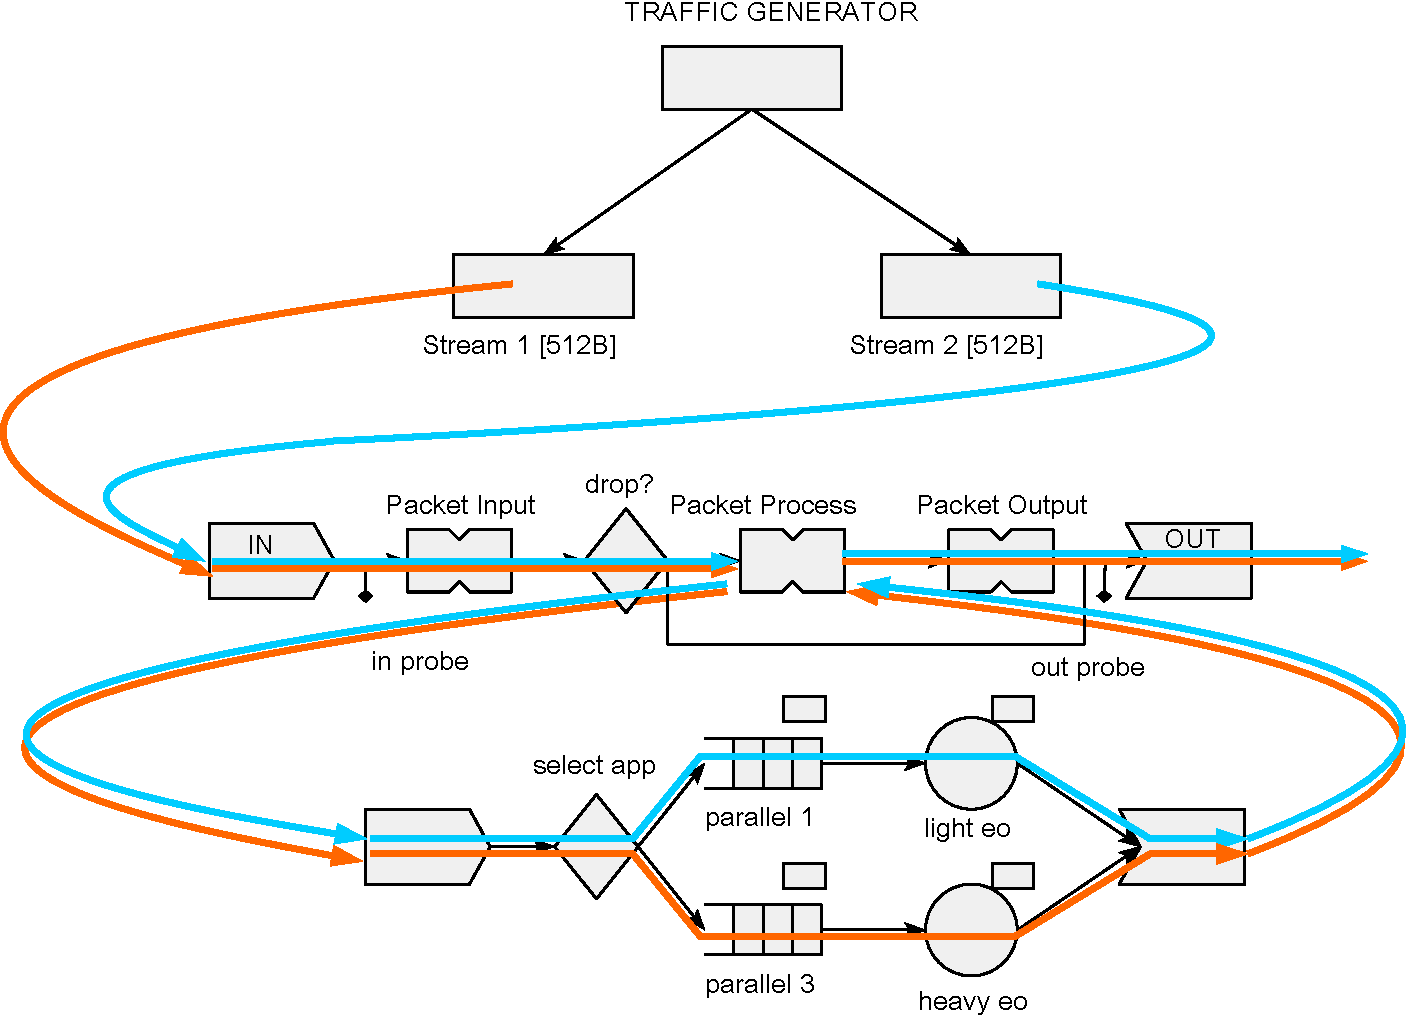
\includegraphics[width=\textwidth]{images/pse-models/exp2-software.pdf}
    \caption{An overview of the workload and software  models used in the experiment 2. The orange and blue paths present the paths of the packets through the system. Each of the flows has its own packet processing application.}
    \label{fig:exp2-software}
  \end{center}
\end{figure}

\subsection{Simulation Measurements}
\label{sec:exp2-simulation-measurements}

The system was simulated with and without the limited coremask on the heavy application processing cores. The data from the probes were then post-processed. Figures~\ref{fig:exp2-app1-no-coremask-latency} and~\ref{fig:exp2-app2-no-coremask-latency} present the data from the simulation without coremask, for the heavy and light flow, respectively. The latency of the heavy flow packets is between 80$\mu$s and 340$\mu$s throughout the simulation. The throughput of the heavy application is 0.214GBps.

\begin{figure}[]
  \begin{center}
    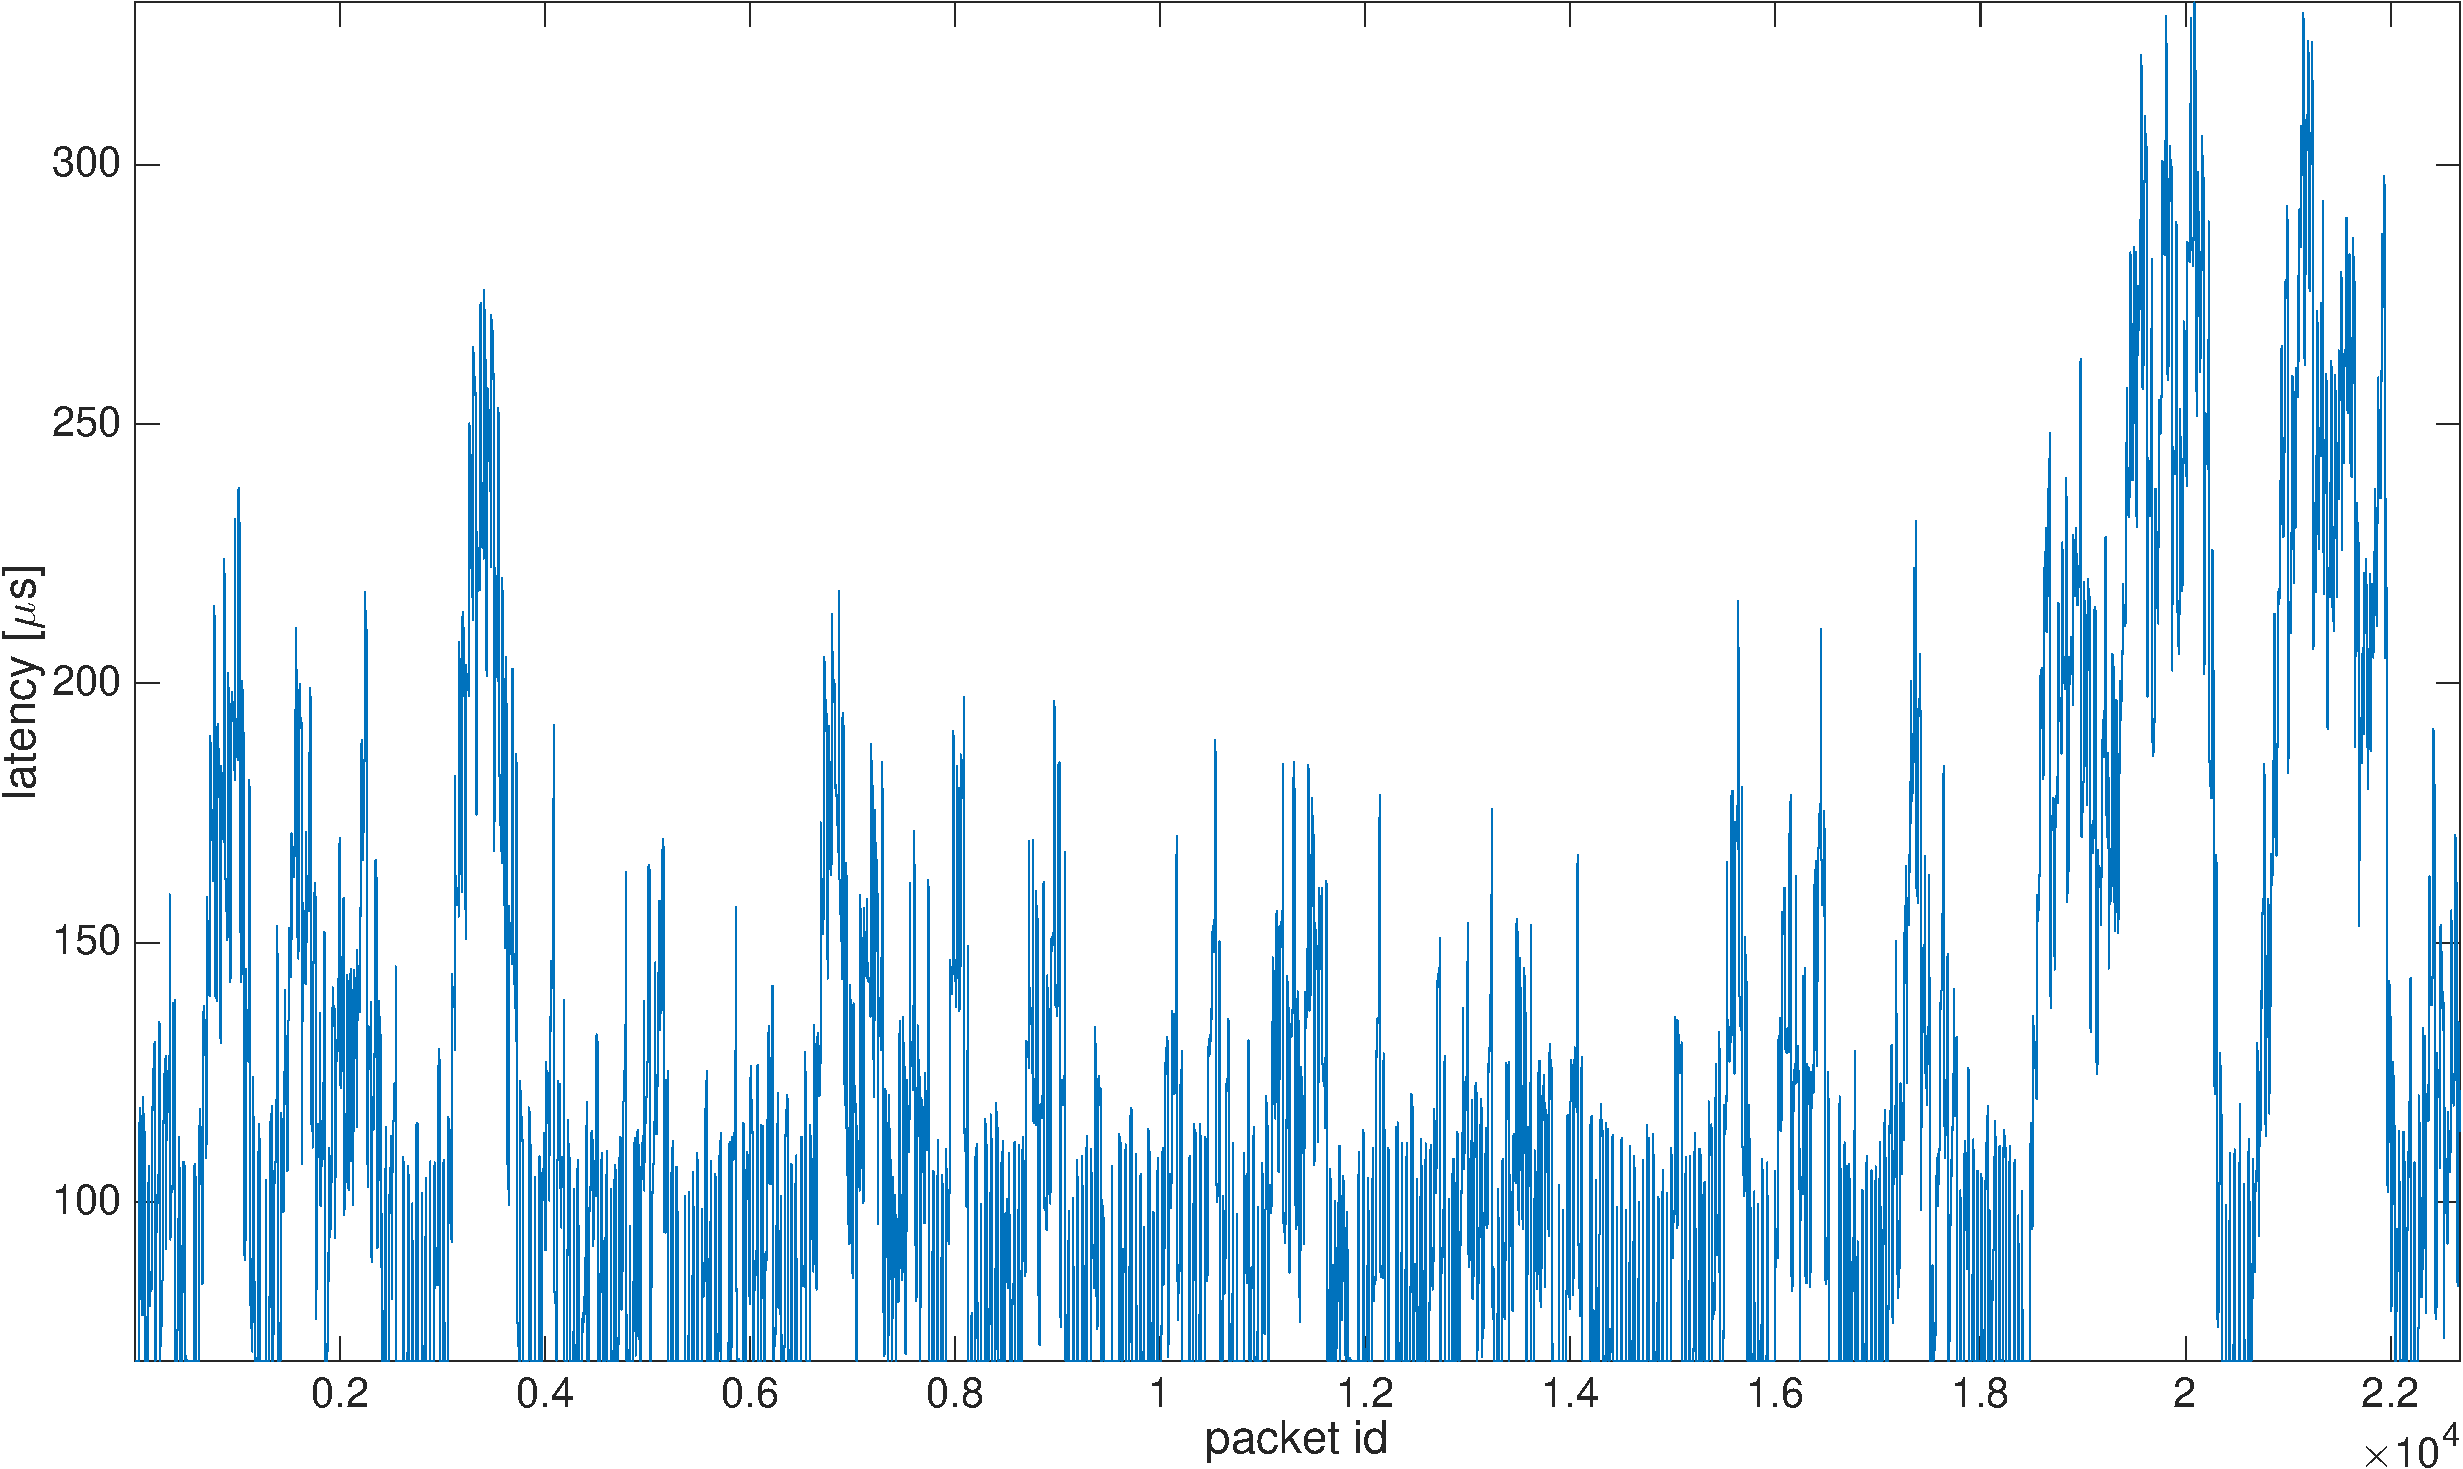
\includegraphics[width=\textwidth]{images/experiment/exp2-app1-no-coremask-latency.pdf}
    \caption{Latencies of the heavy flow packets, without coremask.}
    \label{fig:exp2-app1-no-coremask-latency}
  \end{center}
\end{figure}

\begin{figure}[]
  \begin{center}
    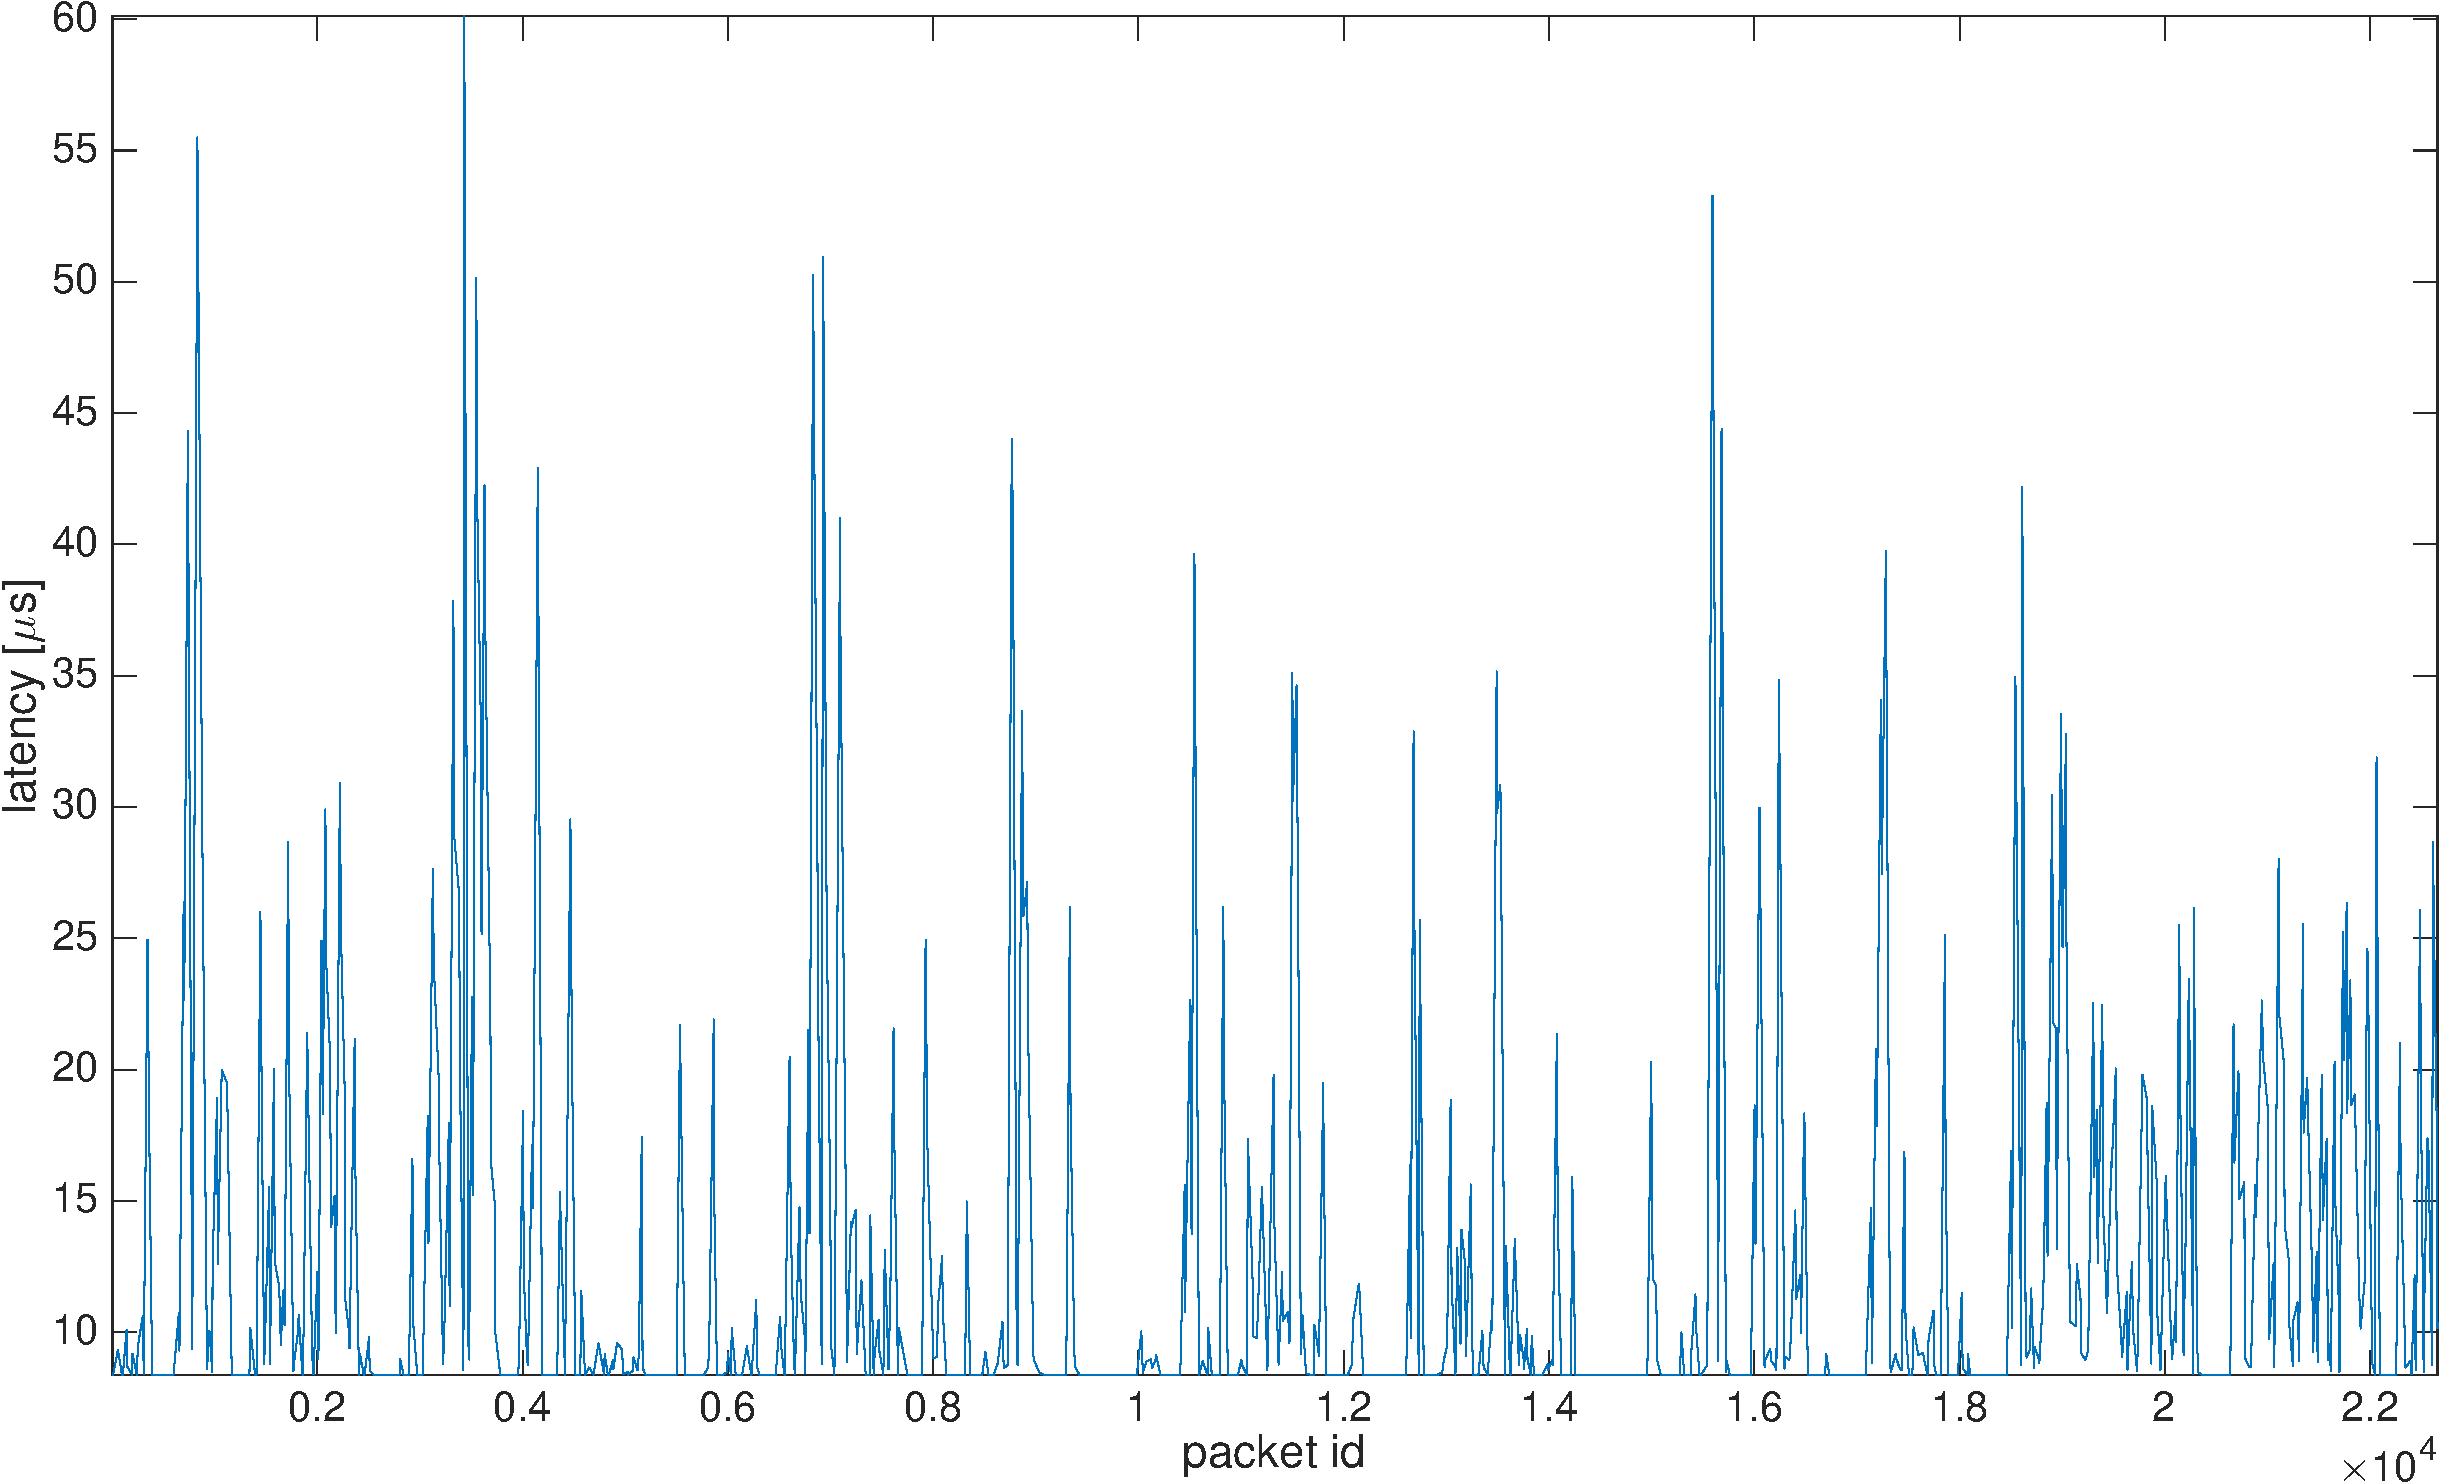
\includegraphics[width=\textwidth]{images/experiment/exp2-app2-no-coremask-latency.pdf}
    \caption{Latencies of the light flow packets, without coremask. The worst-case latencies are almost ten-fold compared to the best-case.}
    \label{fig:exp2-app2-no-coremask-latency}
  \end{center}
\end{figure}

In the second simulation, we use a modified coremask for the heavy application, i.e. dedicating one of the cores for the light application processing. The resulting latencies of the heavy and light flow are presented in Figures~\ref{fig:exp2-app1-is-coremask-latency} and~\ref{fig:exp2-app2-is-coremask-latency}, respectively. The light flow's worst-case packet latencies stay below 12$\mu$s. The throughput of the heavy application is 0.212GBps.

\begin{figure}[]
  \begin{center}
    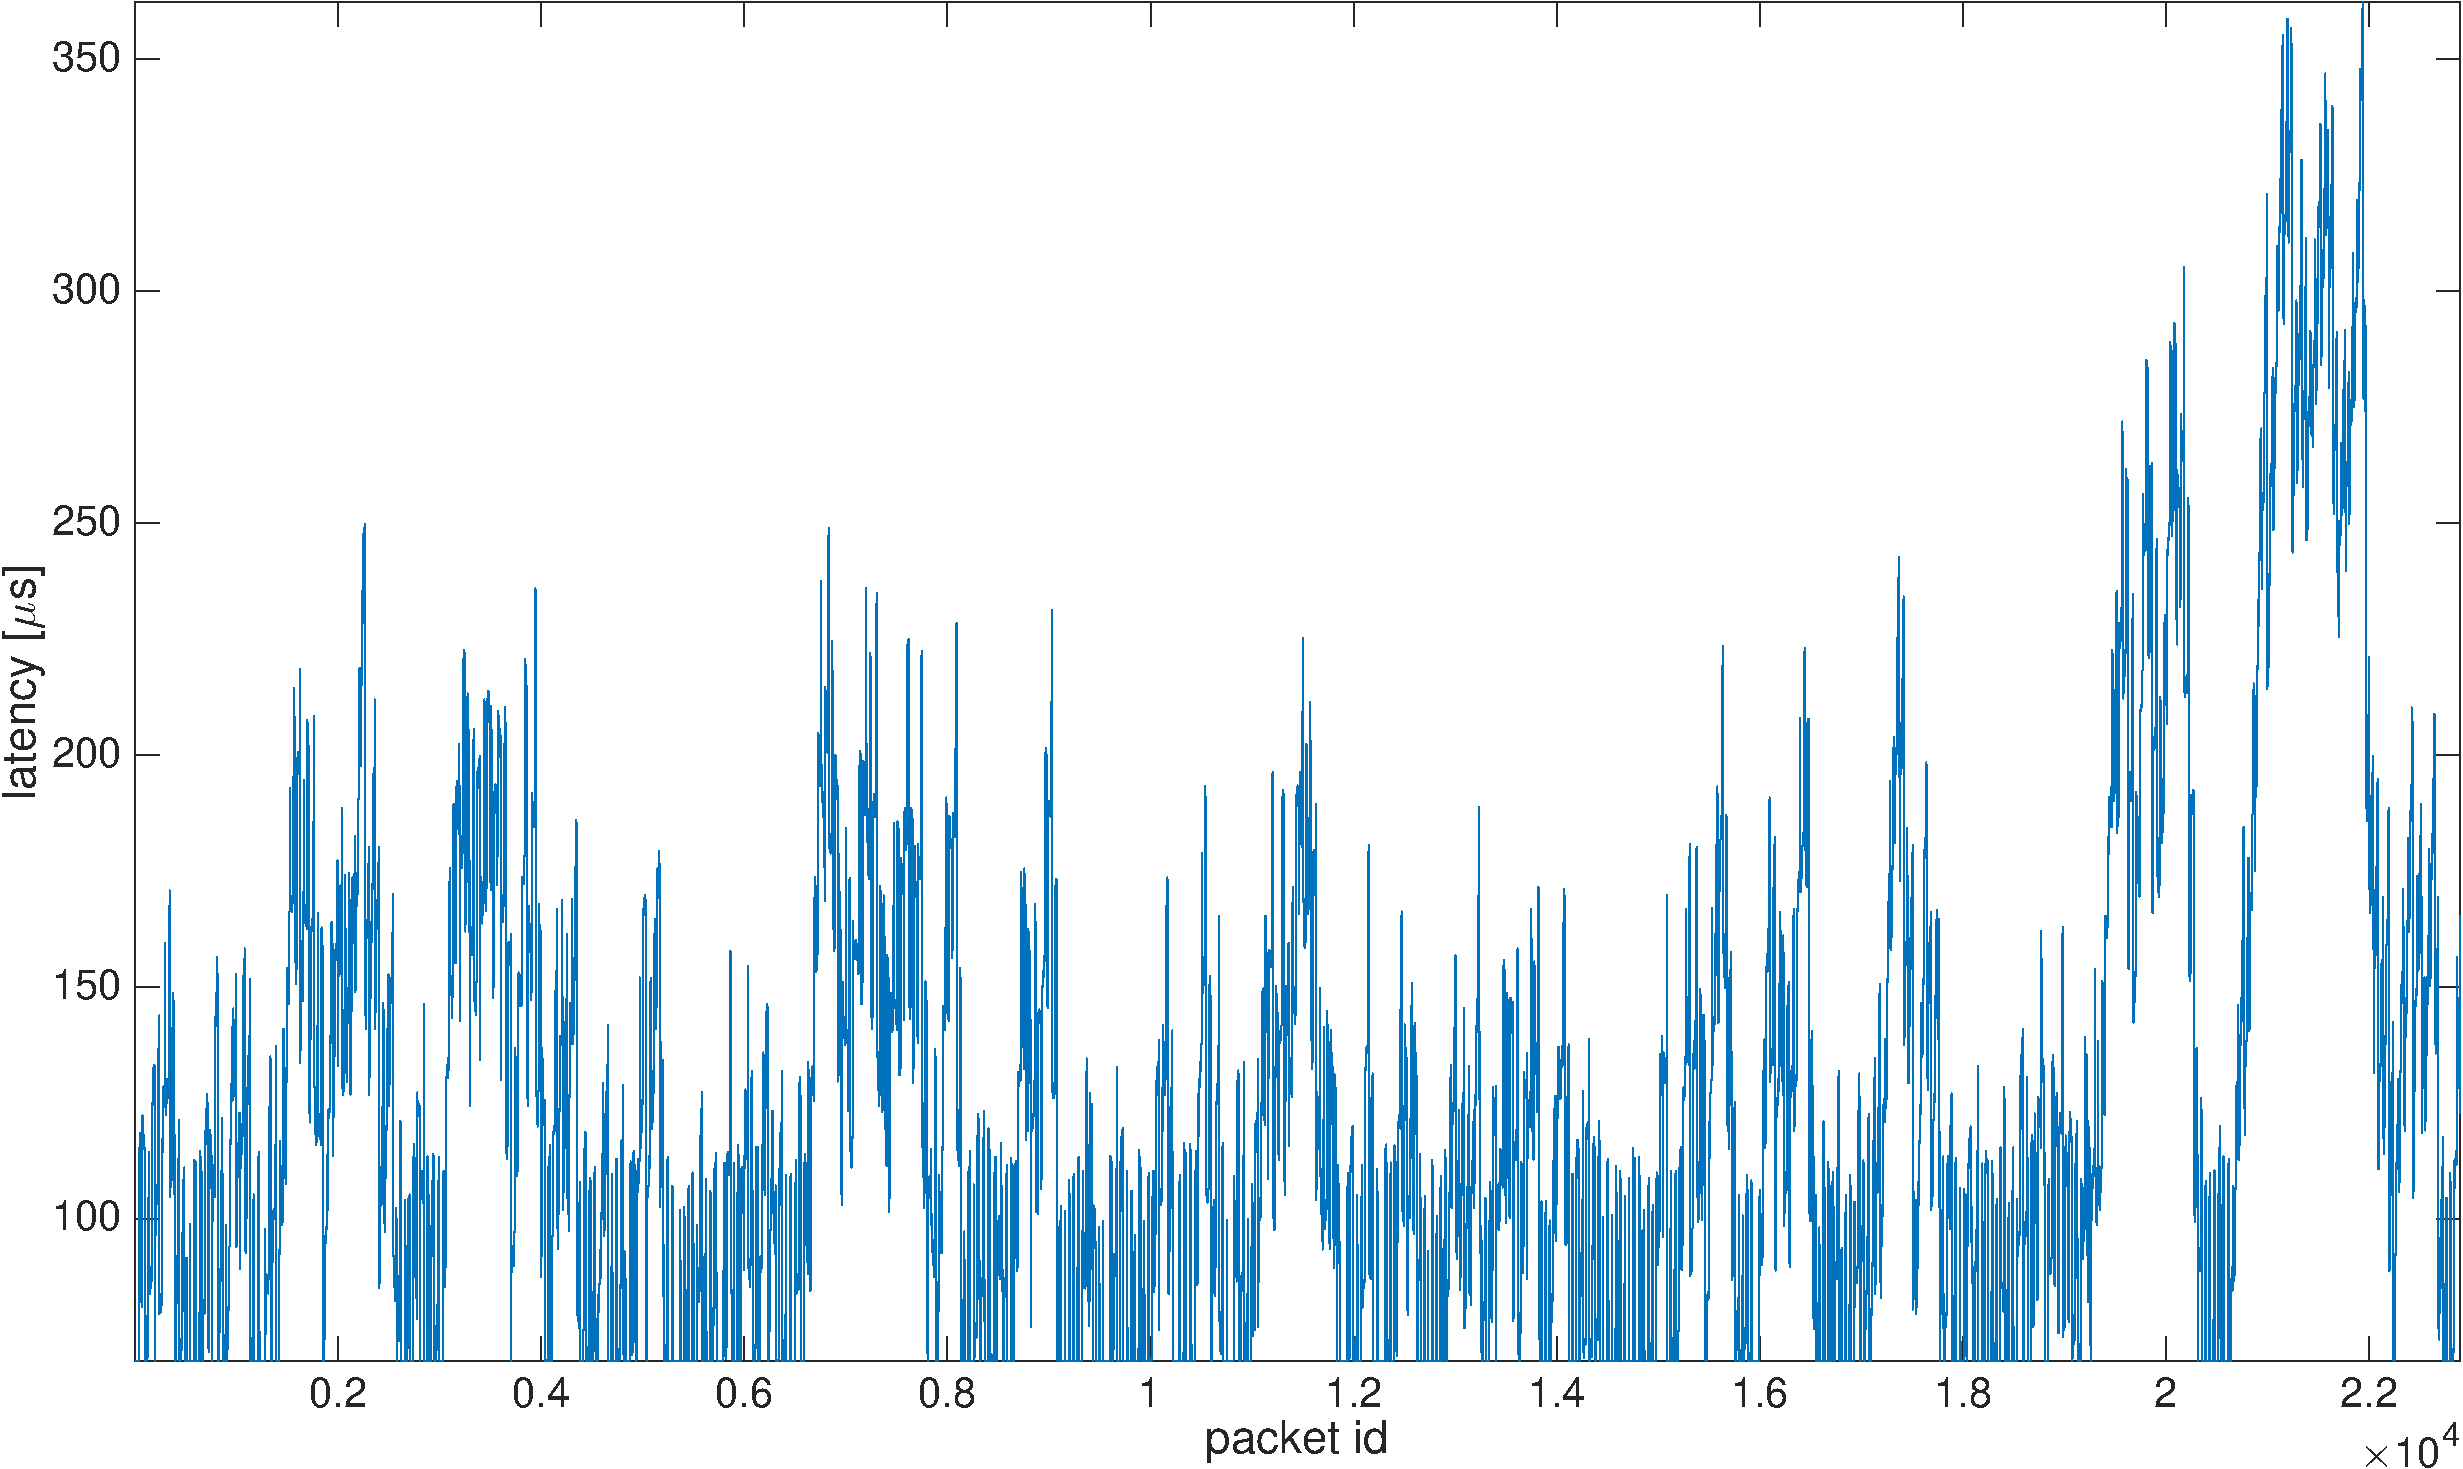
\includegraphics[width=\textwidth]{images/experiment/exp2-app1-is-coremask-latency.pdf}
    \caption{Latencies of the heavy flow packets. One of the cores is dedicated for the light flow.}
    \label{fig:exp2-app1-is-coremask-latency}
  \end{center}
\end{figure}

\begin{figure}[]
  \begin{center}
    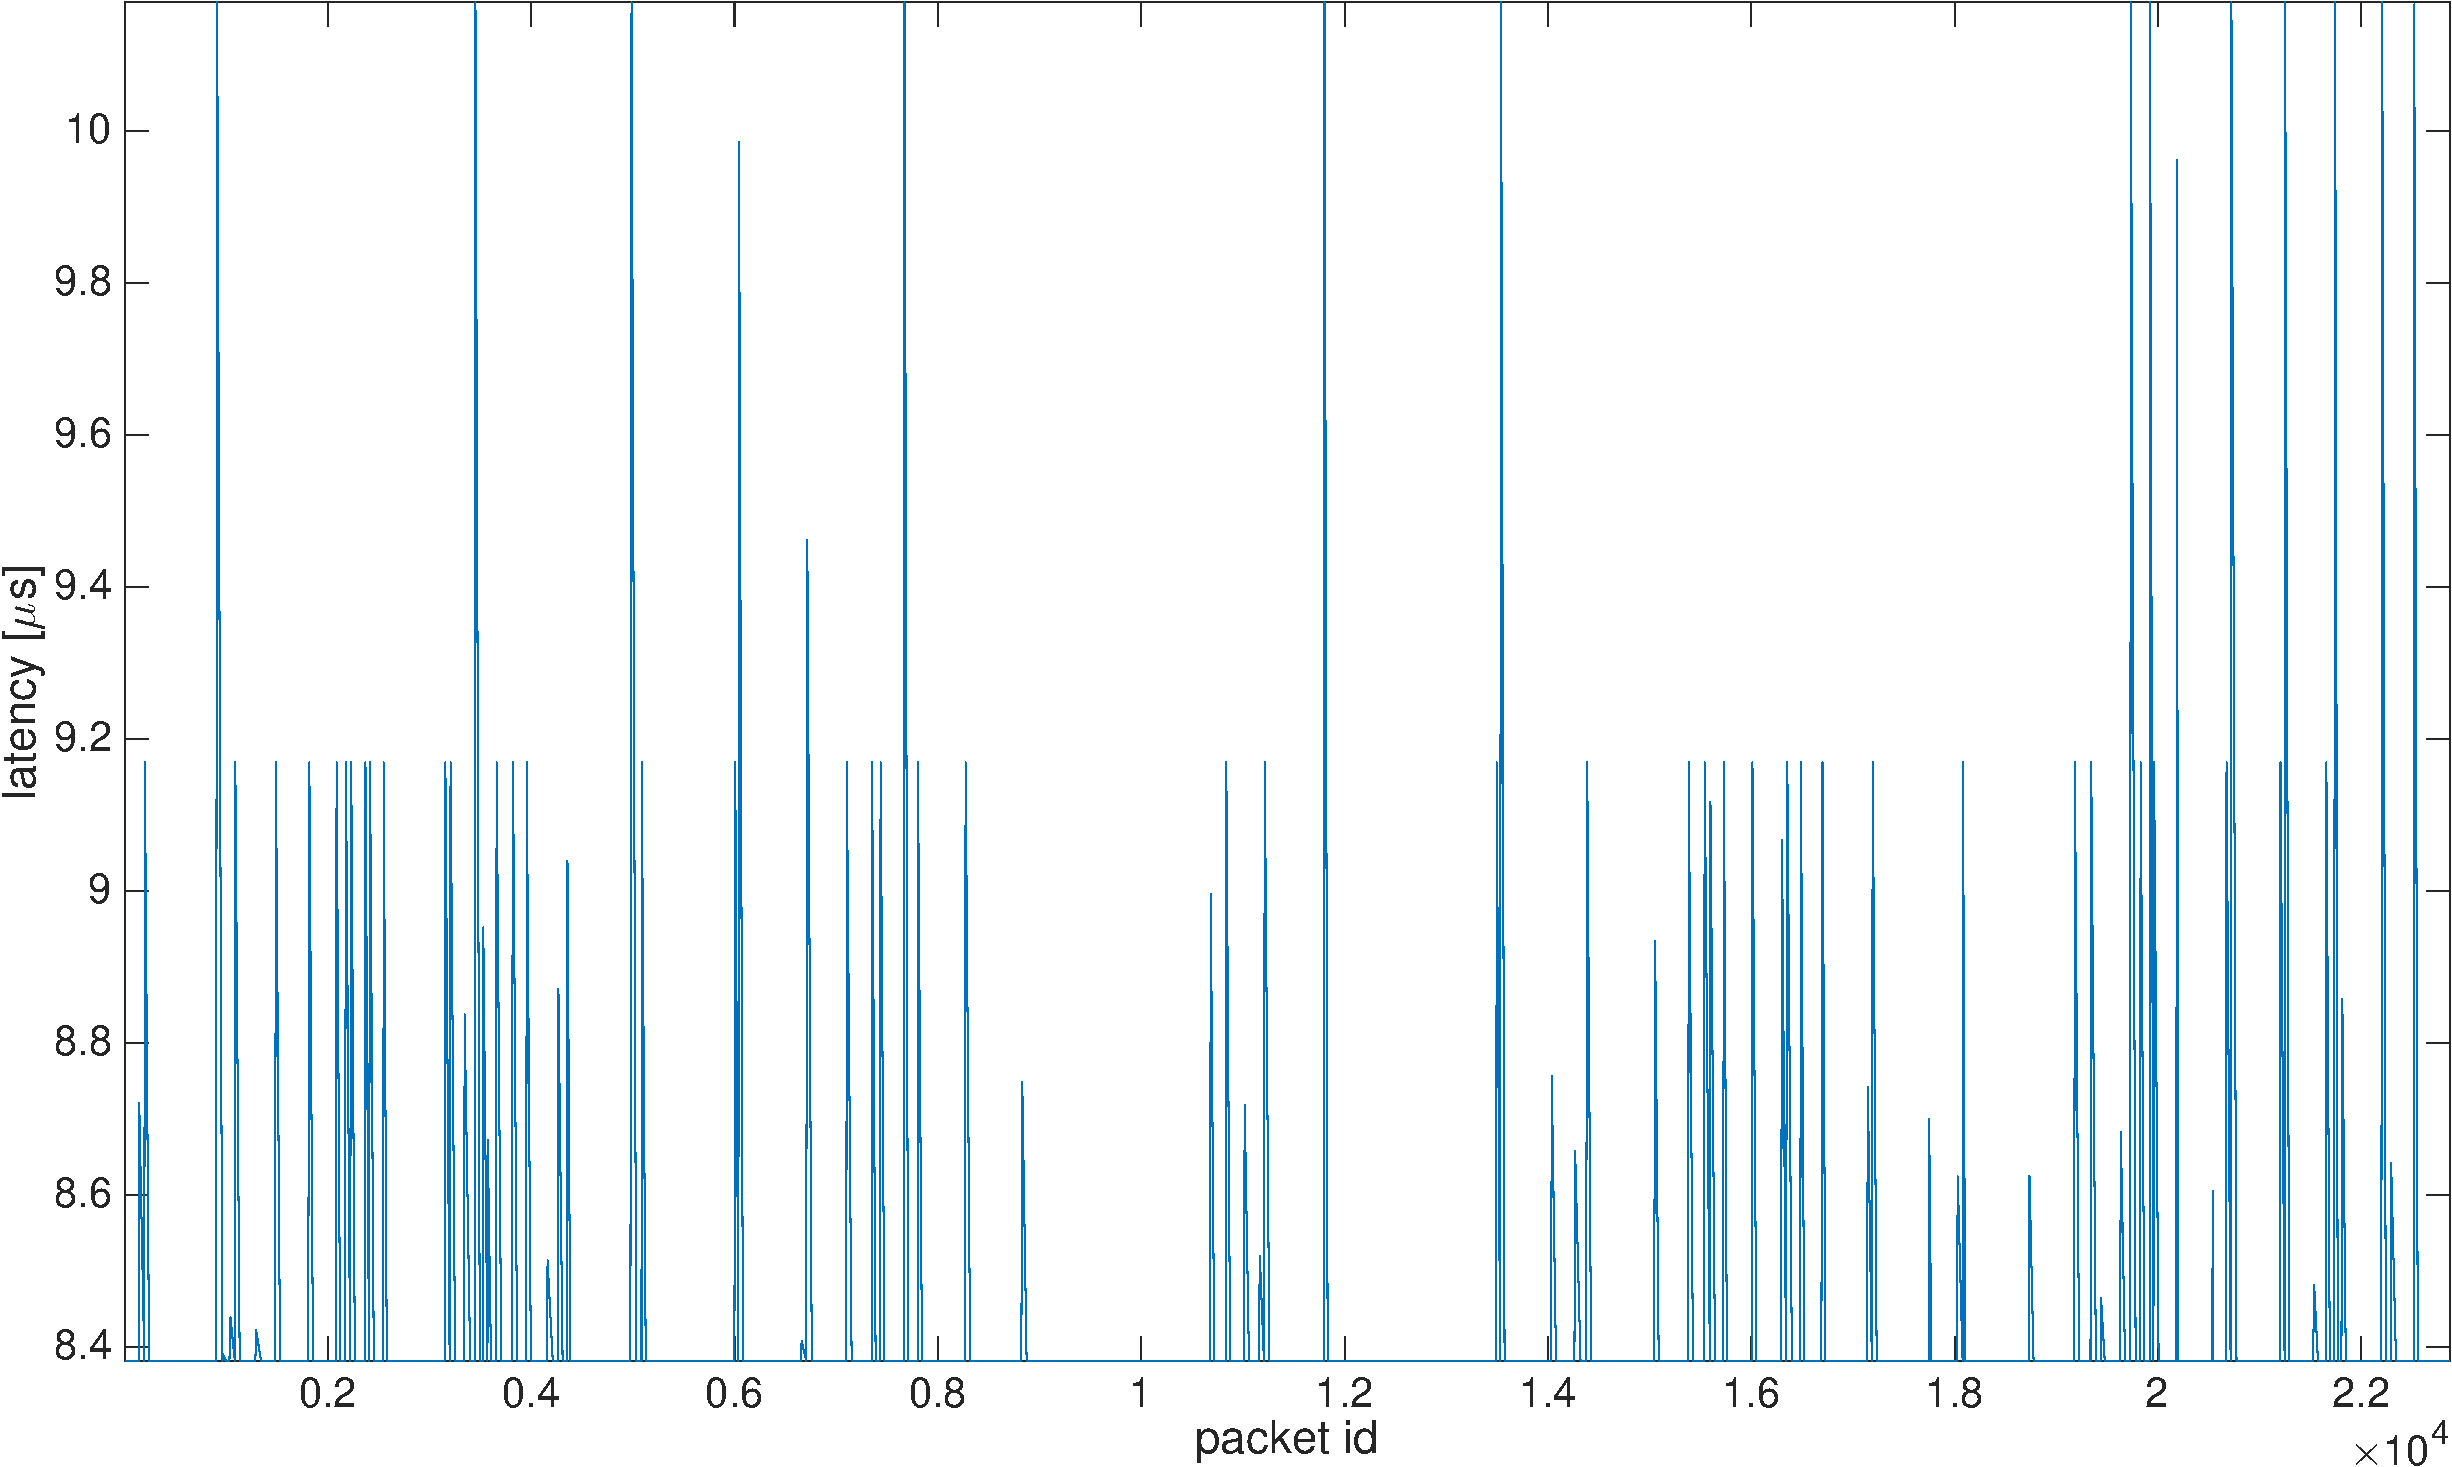
\includegraphics[width=\textwidth]{images/experiment/exp2-app2-is-coremask-latency.pdf}
    \caption{Latencies of the light flow packets. One of the cores is dedicated for the light flow. The worst-case latencies are less than 50\% higher than of the best-case.}
    \label{fig:exp2-app2-is-coremask-latency}
  \end{center}
\end{figure}

\section{Results}

% TODO: simulation methods can speed up the modeling work by abstracting the system and decoupling the complex hardware and software models, while also maintaining the correct behavior of the system under study.

% TODO: comment on simulation times?
The experiments present a proof of concept of the implemented PSE's plugin code mechanism and the model of the reference NPU. In both experiments, the model acts as expected.

The first experiment, presents the use the global queue information to control the resource provision based on global queue priorities and disciplines. As seen in the Figures~\ref{fig:app1-queue2} and~\ref{fig:app1-latency}, the second processing step produces a bottleneck to the system. This happens due to the atomicity of the second processing queue, forcing heavy processing of the packets one at a time. By dividing the atomic processing step into a smaller atomic part and larger parallel part, the latency of the system should be reduced, as the atomic part of the processing can be done faster, and the cores can fully be utilized by the heavier parallel part of the second processing step. The measurements results of the second application, as shown in the Figures~\ref{fig:app2-queue2} and~\ref{fig:app2-latency}, validate this behavior.

The second experiment presents the use of queue coremasks, to control the use of specific hardware resources, through the software model. As shown in the Figure~\ref{fig:exp2-app2-no-coremask-latency}, without limiting the coremask, the light flow packets can be processed in 8$\mu$s at best. However, in the worst-case, when all the cores are processing heavy flow packets, the light flow packet latency is almost ten-fold compared to the best-case latency, 61$\mu$s. By dedicating a processing core for the light flow, we sacrifice the throughput of the heavy flow in order to reduce the worst-case latency of the light flow. As shown in the Figure~\ref{fig:exp2-app2-is-coremask-latency}, changing the coremask in the software model removes the bottleneck from the system. The light flow's worst-case packet latencies can be reduced to less than 50\% higher than of the best-case, while the heavy flow's throughput drops only 2\% compared to the non-coremask processing.

The experiments also highlight the PSE's ability to decouple the hardware and software model. All the changes in the experiment applications can be done through the four software model files. Once the resource provision model and the high level resource usage models are built, the application developers can prototype the system with by modifying only the software and workload parts of the model corresponding the real software applications written in task-based programming models, such as Open Event-Machine. At the same time, the hardware developers can work on the model parts corresponding to the real hardware.

According to the experiment results, the PSE's resource network concept, extended with user-defined queue disciplines, seems to be provide the desired flexibility, both in the abstraction level and the modularity, for modeling complex hardware and software co-scheduled manycore systems, such as the reference network processing unit. More importantly, the plugin code mechanism extends to any resource network based simulation task, providing flexibility, hopefully allowing even more complex systems to be modeled.

%%% Local Variables:
%%% mode: latex
%%% TeX-master: "thesis-hartikainen"
%%% End:

% TODO
% Goals
%   - network processing system ok, clusteri koostuisi useammasta noodista
%   - addressed entity -> kutsutaan nodeksi
%   - node ihan hyva bladesta, processing element viittaa yhteen ytimeen
%   - dipassa NPU, blade kannattaa yhten�ist��
%   - kannattaa luoda pikkasen priorisoinnin kuvaa:
%     - tilanne on se ett� tavoitteet on kahtalaiset
%     - NPU ymm�rryksell� on oma arvonsa
%     - Simuloinnin ymm�rryksell� on oma arvonsa
%     - Latenssip��m��r�t on subgoals, arvo tulee yo. goalien kautta
%     - Se ett� ymm�rret��n delay-rakennetta palvelee molempia:
%       - hajautetun verkkoprosessoinnin ymm�rryst�, sek� simuloinnin ymm�rryst�
%       - Kysymys on ett� mitk� arvot? Kaikkea pystyy tekee, mutta ei ehdi
%       - Mik� on t�rke��, miten/mitk� mittaukset tukee molempia p��m��ri�
%       - Jos mittaus on ty�l�s ja tukee vain toista, kannattaa j�tt�� tekem�tt�

\chapter{Discussion}
\label{chapter:discussion}
\todo[inline]{TODO: this chapter is still undone!}

This chapter discusses the results of our work. First, we present the challenges within the topic of the thesis. The discoveries section discusses the findings made during the thesis. In related work, we summarize the related work on the field of our study. Finally, in the future work section, we propose few possible future directions on our topic of research.

\section{Challenges}
% JUSSI
% Yleisesti ongelma, eli fogi ja cloudi vaatii tehokasta pakettiprosessointia -> performanssianalyysi t�rkeet� -> koska pakettisysteemit ja MPSoCit on vaikeita hardware-tason systeemej� niin analyyttinen analyysi ja mittaaminen usein vaikeeta -> simulaatio t�rkeet�

% Ja ett� fog/cloud jm�t IoT skaalassa ovat monimutkaisia. Niin monimutkaisia, ett� niist� ei usein voi rakentaa protoa ennen jm�n deploymentti�.

% Mallinnuksessa sopiva abstraktiotaso keskeist�. Liian tarkat abstraktiot hidastavat simulaatiota, kun taas liian korkeat antavat summittaisia tuloksia. Lis�ksi k�ytett�vyys, mallinuksen "nopeus", jne..

% Simulaatiota varten t�ytyy pysty� mallintamaan tehokkaammin monimutkasia resursseja, kuten schedulereita
% Simulaatioiden koko kasvaa -> tarvitaan skaalaautuvia simulaattoreita (parallelisoituminen)
% T�m� johtuu tietenkin mallinnettavien jmien kompleksisuuden kasvusta.

Today's packet processing system face an ever-increasing number of packets requiring more and more complex processing. Short development cycles and fast revisioning of the systems have become necessity, as the vendors face fast changes in technology, dynamic customer requirements, and pressure for time-to-market. To answer these requirements, especially with the tightening energy limitations, the packet processing systems are build as a multiprocessor system-on-chips (MPSoC's), called network processing units. Network processing units are optimized for high-speed network packet processing at wire-speeds of multi-Gbps, while at the same time enjoying the generic characteristics similar to general purpose central processing units.

Performance analysis on network processing units is difficult, due to complex non-deterministic behaviour and complex hardware and software interactions of the MPSoC devices, and the dynamic nature of the input data streams. The complexity of today's systems, especially in the scale of cloud and fog computing, is growing to a level where prototyping is not possible.

Modeling is an important tool for the performance analysis of MPSoC systems. The packet processing systems are, in essence, queueing systems. Queue and resource networks are widely studied concepts, often used for packet processing problems. However, the complex low level interactions between the components of MPSoC's make the traditional queue concepts insufficient, while at the same time the exact measurements may be unsuitable, especially in the early stage of the system development.

One way to address this problem, is to extend the resource networks with more flexible queue discplines and methods for modeling parallelism, to correctly mimic the behaviour of complex MPSoC based packet processing systems. More complex queue disciplines and MPSoC behaviour force the use of simulation methods to execute the models.

Correct abstaction level is one of the key elements of modeling. Too detailed models are intractable and require time consuming simulations, while too high level abstractions hide the sought characteristics of the system, resulting in inadequate results.

\todo[inline]{Simulation tracing?}
\todo[inline]{Parallel simulation is problematic}

% Efficient packet processing is one of the major challenges as the computation is moving away from the end-devices, towards cloud and fog. The performance requirements for the packet processing systems are high. To answer these requirements, especially with the tightening energy limitations, the packet processing systems are build as a multiprocessor system-on-chips (MPSoC's). The interconnections between the MPSoC systems' resources require sound solutions on a low system levels. Moving the data plane processing into hardware fast path, is often the only viable solution for answering the latency and packet processing requirements with limited energy consumption.

% The performance analysis of these systems is hard, due to the complex non-deterministic behaviour of the MPSoC devices and the dynamic nature of the input data streams. The non-deterministic behaviour in MPSoC systems is a result of parallelism, communication delays, complex memory systems, and scheduling mechanisms.


\section{Discoveries}
% Discoveries
% PSE:ll� voidaan mallintaa vaikeampiakin hardware interactioista suht intuitiivisesti (ja mahdollisesti my�s tehokkaasti)
% Valitettavaa, mutta mulla ei oikeestaan tuu mit��n sen suurempia discoveryj� mieleen t�n ty�n tuloksena...
% Tai ett� laajentamalla perinteist� resurssiverkkokonseptia globaalilla skedulointi plugarilla, sill� voidaan mallintaa task based processinkia hardware scheduloiduilla alustoilla, tms..

\todo[inline]{Resource network models, extended with more complex queuing disciplines and support for modeling task parallelism, seem to be adequate for modeling complex hardware and software interactions of a modern MPSoC network processing systems}
\todo[inline]{
PSE provides an efficient way of simulating MPSoC systems.
PSE decouples the hardware and software presentation of the models, enabling intuitive, and fast modeling}

% The PSE extensions and experiments implemented during the thesis project, were presented at ParallaX project fall meeting. Based on the feedback received from the participants, PSE has potential use cases in the simulation of the packet processing systems. Especially the clarity of the simulation models, decoupling of the software and hardware models, and the plugin interface, received wide interest.

% Based on the feedback, and our own observations during the development of PSE, we believe that the traditional resource network concept will be an intriguing tool for modeling and simulation of task based processing on hardware scheduled manycore platforms.

\section{Related Work}
% Related Work
% T�h�n varmaan ois kiva kaivaa jotain esim. EPC tai vastaavia simulaatiojuttuja esimerkiks?
% Lis�ks ajattelin esitell� erilaisia simulaattoreita samaan tyyliin kun sunkin related workissa
% Jotain jos l�ytyy j�rjestelmien mallinnuksesta niin hyv� ois.

\todo[inline]{add more stuff on system simulation?}

Simulation is a widely used method in performance analysis of datacenter components. There exists multitude of research in the field of cloud computing and simulation. Various methods, tools, and approaches have been implemented in attempt to balance between competing goals, and cope with a specific subset of the problem space.

Cloud datacenter simulators are used for simulation the critical parts of cloud datacenter. CloudSim~\cite{Calheiros:2011:Cloudsim}, for example, is a toolset for modeling and simulation of cloud computing infrastructure and application services. CloudSim can be used for simulating large scale datacenters, virtualized server hosts with customizable provisioning policies, energy-aware computational resources, data center network topologies and message-passing applications. Various different projects extend the CloudSim API for more detailed performance analysis of different parts fo the cloud system: CloudSimEx enables simulation of MapReduce jobs and CloudAnalyst~\cite{Wickremasinghe:2010:CloudAnalyst} enables simulation of large-scale cloud applications in terms of geographic distribution.

When moving towards the fog, the performance of mobile network technologies becomes important. In~\cite{Ikuno:2010:LTE}, Ikuno et al. present a Matlab based simulation software for the system level LTE networks.

\section{Future Work}
% JUSSI
% Virtualisaation simuloiminen? T�� vaikuttaa mun mielest� t�rkeelt� mutta ne oikein keksi miten tota pit�is purkaa
% Vois tietty olla future workiss�. Jotain tyyliin: virtualisointien (laskenta, tiedonsiirto, yms) mallinnus vaatisi lis�� tasoja resurssiverkkoparadigmaan.

% Varmaan jotain yleisesti fogista ja vastaavasta? Esim. ett� toi meid�n systeemi vois olla osa sellasta experimentti� josta puhuttiin alkuvuodesta
% Ehk� t�nne ennemmin tuo virtualisointi asia, ja jos jotain vastaavaa l�ytyy kanssa.
% Ja jotain yleisesti yh� monimutkaistuvista j�rjestelmist�, ja j�rjestelmien j�rjestelmist�. Internet kokoluokan ongelmista.

\todo[inline]{Modeling virtualized systems? Modeling of virutalization (computing, communication, etc..) Requires more levels to the resource network paradigm.}

As we have shown in this work, the resource network methodology extended with the customized plugin code interaface, can be used for modeling more complex task-based application hardware scheduled manycore systems. The flexibility of PSE, and resource networks, enable simulation of large scale systems on many different parts of the cloud computing context. However, there are certain limitations with the tool as well.

Simulation of larger systems, such as the network processing unit presented in this work, in larger scale, let alone full scale datacenter networks or complex IoT applications that consist large number of different components, with the current implemenation of PSE are not feasible. This is mainly due to the inefficient implementation of the threads executing tasks, and the memory systems. The threads are fairly heavy structures to handle the tasks, in the context of large-scale simulations. These could, for example, be replaced with similar structures as Akka frameworks' actors.

Parallelization of the simulator is one of the most important steps towards efficient, massive scale, simulations. This is a widely researched topic in itself, and faces multiple challenges, not only the ones faced with parallelization in general, but also the simulators' nature make the problem non-trivial.


%%% Local Variables:
%%% mode: latex
%%% TeX-master: "thesis-hartikainen"
%%% End:

\chapter{Conclusions}
\label{chapter:conclusions}

\todo[inline]{write conclusions}

%%% Local Variables:
%%% mode: latex
%%% TeX-master: "thesis-hartikainen"
%%% End:



% Load the bibliographic references
% ------------------------------------------------------------------
% You can use several .bib files:
% \bibliography{thesis_sources,ietf_sources}
% \bibliography{sources}
% \nocite{*}
% \todo[inline]{remove nocite}
\printbibliography
% Appendices go here
% ------------------------------------------------------------------
% If you do not have appendices, comment out the following lines
% \appendix
% \chapter{First appendix}
\label{chapter:first-appendix}
\lstinputlisting[caption=RNS\_use\_device,
                 label=lst:RNS-use-device]{listings/RNS_use_device.c}

RNS\_use\_device in~\ref{lst:RNS-use-device} reserves the resource, delays the process (i.e. the task) and releases the resource for other processes.

\lstinputlisting[caption=RNS\_demand\_device,
                 label=lst:RNS-demand-device]{listings/RNS_demand_device.c}

RNS\_demand\_device routine in~\ref{lst:RNS-demand-device} is a simple wrapper routine, that converts the demanded service amount (service\_amount) into corresponding service time, based on the device entity speed (d-$\textgreater$speed). It then calls the RNS\_use\_device routine with the resulting service time.

\lstinputlisting[caption=RNS\_reserve\_resource,
                 label=lst:RNS-reserve-resource]{listings/RNS_reserve_resource.c}

\ref{lst:RNS-reserve-resource} summarizes the RNS\_reserve\_resource routine. RNS\_reserve\_resource calls the reserve function bound to the resource entity as explained in section \ref{TODO}. The reserve function assigns the task either in the resource's processing queue or waiting queue.

If the reserve function assigns the task to the waiting queue, the thread yields the execution to the scheduler.

\lstinputlisting[caption=RNS\_delay\_process,
                 label=lst:RNS-delay-process]{listings/RNS_delay_process.c}
\lstinputlisting[caption=RNS\_release\_resource,
                 label=lst:RNS-release-resource]{listings/RNS_release_resource.c}

%%% Local Variables:
%%% mode: latex
%%% TeX-master: "thesis-hartikainen.tex"
%%% End:


% End of document!
% ------------------------------------------------------------------
% The LastPage package automatically places a label on the last page.
% That works better than placing a label here manually, because the
% label might not go to the actual last page, if LaTeX needs to place
% floats (that is, figures, tables, and such) to the end of the
% document.
\end{document}

%%% Local Variables:
%%% mode: latex
%%% TeX-master: t
%%% End:
